\documentclass[a4paper,10pt]{report}
% ---- graphiques
\usepackage[pdftex]{graphicx}
\usepackage{wrapfig}
\usepackage{color}
%\usepackage{hyperref}

% for latex2html
\usepackage{html}

% for accents
\usepackage[latin1]{inputenc}
\usepackage[T1]{fontenc}

\usepackage{algorithm}
\usepackage{algorithmic}

\definecolor{darkgreen}{rgb}{0,0.4,0}
\definecolor{darkblue}{rgb}{0,0,0.4}
\definecolor{darkgray}{rgb}{0.2,0.2,0.2}

% ---- inclusion de codes
\usepackage{listings}
\lstset{showstringspaces=false,tabsize=4,basicstyle=\scriptsize\sffamily,breaklines=true,breakatwhitespace=true,framexleftmargin=5mm, frame=shadowbox, framesep=1pt,rulesepcolor=\color{darkgray},rulesep=.5pt,keywordstyle=\bf\color{blue},commentstyle=\color{magenta},stringstyle=\color{red},numbers=left,numberstyle=\tiny,numbersep=5pt,columns=flexible}

\lstdefinestyle{bash}{language=bash}
\lstdefinestyle{Perl}{language=Perl}
\lstdefinestyle{C++}{language=C++,emph={__global__,__shared__,__syncthreads,blockIdx,threadIdx,float3,float4},emphstyle=\bf\color{darkgreen}}
\lstdefinestyle{DTD}{language=XML}
\lstdefinestyle{XML}{language=XML,usekeywordsintag=false,markfirstintag=true}
%begin{latexonly}
\newcommand{\includecode}[2]{
\lstinputlisting[style=#1]{#2}
}
%end{latexonly}
\begin{htmlonly}
\newcommand{\includecode}[2]{  \htmladdnormallink{#2}{../../#2} }
\end{htmlonly}

%\lstnewenvironment{code}{}{}
\lstnewenvironment{code_bash}{\lstset{style=bash}}{}
\lstnewenvironment{code_perl}{\lstset{style=Perl}}{}
\lstnewenvironment{code_cpp}{\lstset{style=C++}}{}
\lstnewenvironment{code_dtd}{\lstset{style=DTD}}{}
\lstnewenvironment{code_xml}{\lstset{style=XML}}{}

\newcommand{\textcode}[1]{{\sf #1}}



%
\newcommand{\sofa}{SOFA}
\newcommand{\todo}[1]{}
\newcommand{\eg}{\textit{e.g.} }

\renewcommand{\vec}[1]{\ensuremath{\mathbf{#1 }}} % vector
\newcommand{\Vx}{\vec{x} } % position vector
\newcommand{\Vv}{\vec{v} } % velocity vector
\newcommand{\Va}{\vec{a} } % acceleration vector
\newcommand{\Vf}{\vec{f}} % force
\newcommand{\Vdv}{\vec{\delta\Vv}} % change of velocity vector (unknown in implicit CG, and used in constraint solver
\renewcommand{\P}{\mat{P} } % projection to a constrained space.

\newcommand{\JNL}{\mathbf{\mathcal{J}} }     % mapping des positions
\newcommand{\J}{\mat J }                 % mapping lineaire
\newcommand{\M}{\mat M }             % matrice de masse
\newcommand{\K}{\mat K }             % matrice de raideur
\newcommand{\B}{\mat B }             % matrice d'amortissement
\newcommand{\G}{\mat G }             % jacobien des contraintes



% ---- inclusion de codes
\definecolor{darkgreen}{rgb}{0,0.4,0}
\definecolor{darkblue}{rgb}{0,0,0.4}
\definecolor{darkgray}{rgb}{0.2,0.2,0.2}


% macros mathematiques
\newcommand{\ma}[1]{\ensuremath{\mathbf {#1}}}
\newcommand{\ve}[1]{\ensuremath{\mathbf {#1}}}

\usepackage{amsmath}
\usepackage{amsfonts}
\usepackage{amssymb}

% character styles
\newcommand{\bm}[1]{\ensuremath{\mathbf{{#1}}}}
\newcommand{\mcal}[1]{\mbox{$\mathcal #1$}} % rondes math
\newcommand{\bmcal}[1]{\mbox{\boldmath $\mathcal #1$}} % rondes grasses math
\newcommand{\ensemble}[1]{\mbox{$\mathbb{#1}$}}
\newcommand{\RRR}{\mbox{$\ensemble{R}^3$}} 


% d�finitions
\newcommand{\definition}[2]{\index{#1}{\bf #1}: #2}
\newcommand{\voc}[1]{\index{#1}#1}
\newcommand{\bvoc}[1]{\index{#1}{\bf #1}}

% misc
\newcommand{\EV}[1]{\stackrel{\rightarrow}{#1}}  % espace vectoriel
\newcommand{\EA}[1]{#1}                          % espace affine

% vectors, matrices
%\newcommand{\point}[1]{\mbox{$#1$}}          % un point
\newcommand{\point}[1]{\ensuremath{#1}}          % un point
\newcommand{\mat}[1]{\bm{#1}}         % matrice
\newcommand{\matnm}[3]{\bm{#1_{#2\times #3}}}  % matrice n lignes , m colonnes
\newcommand{\vect}[1]{\bm{#1}}        % vecteur 
%\newcommand{\vecf}[1]{\stackrel{\rightarrow}{#1}}  % vecteur avec fleche
\newcommand{\vecf}[1]{\mbox{$\overrightarrow{#1}$}}  % vecteur avec fleche
\newcommand{\ident}[1]{\bm{I_{#1}}}   % identit� en dimension n
\newcommand{\inv}[1]{#1^{-1}}         % matrice inverse
\newcommand{\psinv}[1]{#1^{+}}        % matrice pseudo-inverse
\newcommand{\transp}[1]{#1^T}         % transpos�e de 1
\newcommand{\trace}[1]{tr(#1)}        % trace
\newcommand{\deter}[1]{\mbox{$|#1|$}}       % determinant
\newcommand{\oppvec}[1]{\mbox{$\left( \vect {#1} \wedge \right)$}}  % operateur matriciel de produit vectoriel

% bases, reperes
\newcommand{\vecin}[2]{\mbox{${}^{#2}#1$}}    % vecteur 1 dans repere 2
\newcommand{\Base}[1]{\ensuremath{\mathcal B_{#1}}} % Symbole du repere 1
\newcommand{\chbase}[3]{\mbox{${}_{#2}^{#3}\mat{#1}$}}  % operateur 1 fait le passage de la base 3 vers la base 2
%\newcommand{\pchbase}[2]{\chbase{\mat{B}}{#1}{#2}}  % matrice de passage de la base 2 vers la base 1
\newcommand{\pchbase}[2]{\chbase{B}{#1}{#2}}  % matrice de passage de la base 2 vers la base 1
\newcommand{\Rep}[1]{\ensuremath{\mathcal R_{#1}}} % Symbole du repere 1
\newcommand{\rep}[1]{\Rep{#1}}                 % Symbole du repere 1
%\newcommand{\pchrep}[2]{\chbase{\mat{F}}{#1}{#2}}  % matrice de passage du repere 1 vers le repere 2, F comme Frame
\newcommand{\pchrep}[2]{\chbase{\bm{C}}{#1}{#2}}  % matrice de passage du repere 2 vers le repere 1

%% Operateur de passage du repere 1 par rapport a 2
%\newcommand{\ChgRep}[2]{\mbox{\boldmath $R_{#1}^{#2}$}}

% rotations	
%\newcommand{\rot}[2]{\mbox{$\mat{R}_{#1,#2}$}}      % rotation vectorielle
\newcommand{\rot}[2]{\ensuremath{\mat{R}_{#1,#2}}}      % rotation vectorielle
\newcommand{\rota}[3]{\mbox{$\mat{R}_{#1,#2,#3}$}}  % rotation affine

% translation
\newcommand{\trans}[2]{\mbox{$\chbase{\vect{t}}{#1}{#2}$}} % passage de #1 vers #2 par une translation, ou translation du repere #2 par rapport au repere #1

% vitesses et acc�l�rations
\newcommand{\VRep}[2]{\mbox{\boldmath $\dot R_{#1}^{#2}$}} % vitesse du repere 1 par rapport a 2 
%\newcommand{\Point}[2]{\mbox{\boldmath ${#1}^{#2}$}}  % Coordonnees d'un point 1 dans un repere 2
\newcommand{\Point}[2]{\mbox{$\vecin{\bm{#1}}{#2}$}}  % Coordonnees d'un point 1 dans un repere 2
\newcommand{\VPoint}[2]{\mbox{\boldmath ${\dot #1}_{/#2}$}} % Vitesse d'un point par rapport � un repere
\newcommand{\APoint}[2]{\mbox{\boldmath ${\ddot #1}_{/#2}$}} % Acceleration d'un point par rapport � un repere

% cinematique du solide
\newcommand{\derivedans}[2]{\mbox{$\dot{#1}^{(#2)}$}}  % derivee du vecteur 1 dans repere 2
\newcommand{\fixedans}[2]{\mbox{$#1_{\in #2}$}}        % vecteur 1 fixe dans repere 2
\newcommand{\vecom}{\mbox{$\bm{\Omega}$}}  % omega de 1 par rapport a 2
\newcommand{\vecrot}[2]{\mbox{$\vecom_{#1/#2}$}}  % omega de 1 par rapport a 2
\newcommand{\accrot}[2]{\mbox{$\dot{\vecom}_{#1/#2}$}}  % omega de 1 par rapport a 2
\newcommand{\vfdans}[3]{\mbox{$\vec V^{#2/#3}_{#1}$}}    % vitesse de 1 fixe dans 2 par rapport a 3
\newcommand{\afdans}[3]{\mbox{$\vec \Gamma^{#2/#3}_{#1}$}}    % acceleration de 1 fixe dans 2 par rapport a 3
\newcommand{\vmdans}[2]{\mbox{$\vec V^{/{#2}}_{#1}$}}    % vitesse de 1 mobile dans 2
\newcommand{\amdans}[2]{\mbox{$\vec \Gamma^{/#2}_{#1}$}}    % acceleration de 1 mobile dans 2

% chaines articulees
\newcommand{\liaison}[2]{\mbox{$\mathcal L_{#1,#2}$}}  % liaison du pere 1 vers fils 2 (et repere intermediaire)
\newcommand{\liaisonprime}[2]{\mbox{$\mathcal L'_{#1,#2}$}}  % deuxieme repere intermediaire de la liaison du pere 1 vers fils 2
\newcommand{\liaisonP}[2]{\mbox{$\mathcal L_{#1,#2}$}}  % Repere dans pere 1 de la liaison vers fils 2 
\newcommand{\liaisonC}[2]{\mbox{$\mathcal L'_{#1,#2}$}}  % Repere dans fils de la liaison du pere 1 vers fils 2 
%\newcommand{\transP}[2]{\pchrep{\liaisonP{#1}{#2}}{#1}}  % Matrice du repere dans pere de la liaison du pere 1 vers fils 2 
%\newcommand{\transC}[2]{\pchrep{\liaisonC{#1}{#2}}{#2}}  % Matrice du repere dans pere de la liaison du pere 1 vers fils 2 
%\newcommand{\transPC}[2]{\pchrep{\liaisonC{#1}{#2}}{\liaisonP{#1}{#2}}}  % matrice de passage entre repere liaison dans fils et repere de liaison dans pere
\newcommand{\transP}[2]{\chbase{C_p}{#2}{#1}}  % Matrice du repere dans pere de la liaison du pere 1 vers fils 2 
\newcommand{\transC}[2]{\chbase{C_c}{#2}{#1}}  % Matrice du repere dans pere de la liaison du pere 1 vers fils 2 
\newcommand{\transPC}[2]{\chbase{C_l}{#2}{#1}}  % matrice de passage entre repere liaison dans fils et repere de liaison dans pere
% \pchrep{fils}{pere} = \liaisonP{pere}{fils}\deplPC{pere}{fils}\liaisonC{pere}{fils}

%topology
\newcommand{\mesh}{{\mathcal M}}
\newcommand{\vertices}{{\mathcal V}}
\newcommand{\edges}{{\mathcal E}}
\newcommand{\triangles}{{\mathcal TR}}
\newcommand{\tetrahedra}{{\mathcal T}}
\newcommand{\controls}{{\mathcal C}}
\newcommand{\nvertices}{{ V}}
\newcommand{\nedges}{{ E}}
\newcommand{\ntriangles}{{ TR}}
\newcommand{\ntetrahedra}{{ TE}}
\newcommand{\ncontrols}{{C}}
\newcommand{\control}{{\mathbf C}}
\newcommand{\degree}{{d}}
\newcommand{\euc}{{\rm I\!R}}
\newcommand{\naturalSet}{{\rm I\!N}}

\newcommand{\pctab  }{\hspace{0.15in}      }  % Pseudo-code indentation.
\newcommand{\code}[1]{ 
\begin{makeimage}
\begin{tabbing} \pctab \= \pctab \= \pctab \= \pctab \= \pctab \= \pctab \= \pctab \kill
#1
\end{tabbing}
\end{makeimage}
}
 % Customizations 

% ---- format de page A4
	\setlength{\textwidth }{16cm}	% largeur de ligne
	\setlength{\textheight}{23cm}   % hauteur du texte
	\setlength{\oddsidemargin}{0cm} % marge pages impaires
	\setlength{\evensidemargin}{0cm}% marge pages paires
	\setlength{\topmargin}{0cm} 	

% Title Page
\title{Sofa Documentation\\
\vspace{10mm}\normalsize{Also See \bf{http://www.sofa-framework.org/documentation} } }
\author{The Sofa Team}




\begin{document}
\maketitle

\begin{abstract}	
\sofa{} (Simulation Open Framework Architecture) is an open-source C++ library primarily  targeted at interactive medical simulation.
\sofa{} facilitates collaborations between specialists from various domains, by decomposing complex simulators into components designed independently and organized in a scenegraph data structure.
Each component encapsulates one of the aspects of a simulation, such as the degrees of freedom, the forces and constraints, the differential equations, the main loop algorithms, the linear solvers, the collision detection algorithms or the interaction devices. The simulated objects can be represented using several models, each of them optimized for a different task such as the computation of elastic forces, collision detection, haptics or visual display. To ensure a consistent simulation, these models are synchronized during the simulation using a mapping mechanism.
CPU and GPU implementations can be transparently combined to exploit the computational power of modern hardware architectures.
%Simulations descriptions files can be read from and written to xml files.
As a result of this flexible and efficient architecture, \sofa{} can be used as a test-bed to compare models and algorithms, or as a basis for the development of complex, high-performance simulators.

\end{abstract}

\tableofcontents

\part{Foundation of SOFA}

% This chapter is borrowed from a stand-alone document defined in directory introduction/
\chapter{Introduction to \sofa}

\graphicspath{{../introduction/}}  % to include images


% \begin{abstract}
% This is the documentation of the SOFA library. Chapter~\ref{chapter:pba} gives theoretical background on physically-based animation. Chapter~\ref{chapter:as} shows how to implement simulations using \sofa. Chapter~\ref{chapter:es} describes how to integrate new components in \sofa.
% \end{abstract}

%\tableofcontents


\section{Brief overview}
\sofa is an open-source C++ library for physical simulation, primarily targeted to medical simulation.
It can be used as an external library in another program, or using one of the associated GUI applications.

The main feature of \sofa  compared with other libraries is its high flexibility. 
It allows the use of multiple interacting geometrical models of the same object, typically, a mechanical model with mass and constitutive laws, a collision model with simple geometry, and a visual model with detailed geometry and rendering parameters. 
Each model can be designed independently of the others. 
During run-time, consistency is maintained using mappings.


Additionally, \sofa  scenes are modeled using a data structure similar to hierarchical scene graphs commonly used in graphics libraries. 
This allows the splitting of the physical objects into collections of independent components, each of them describing one feature of the model, such as mass, force functions and constraints.
For example, you can replace spring forces with finite element forces by simply replacing one component with another, all the rest (mass, collision geometry, time integration, etc.) remaining unchanged.

Moreover, simulation algorithms, such as time integration or collision detection and modeling, are also modeled as components in the scene graph. 
This provides us with the same flexibility for algorithms as for models.

Flexibility allows one to focus on its own domain of competence, while re-using the other's contributions on other topics.
However, efficiency is a major issue, and we have tried to design a framework which allows both efficiency and flexibility.



\section{Commented example} \label{sec:commentedExample}
Figure~\ref{fig:mixedPendulum} shows a simple scene composed of two different objects, one rigid body and one particle system, and linked by a spring.
\begin{figure}
 \centering
 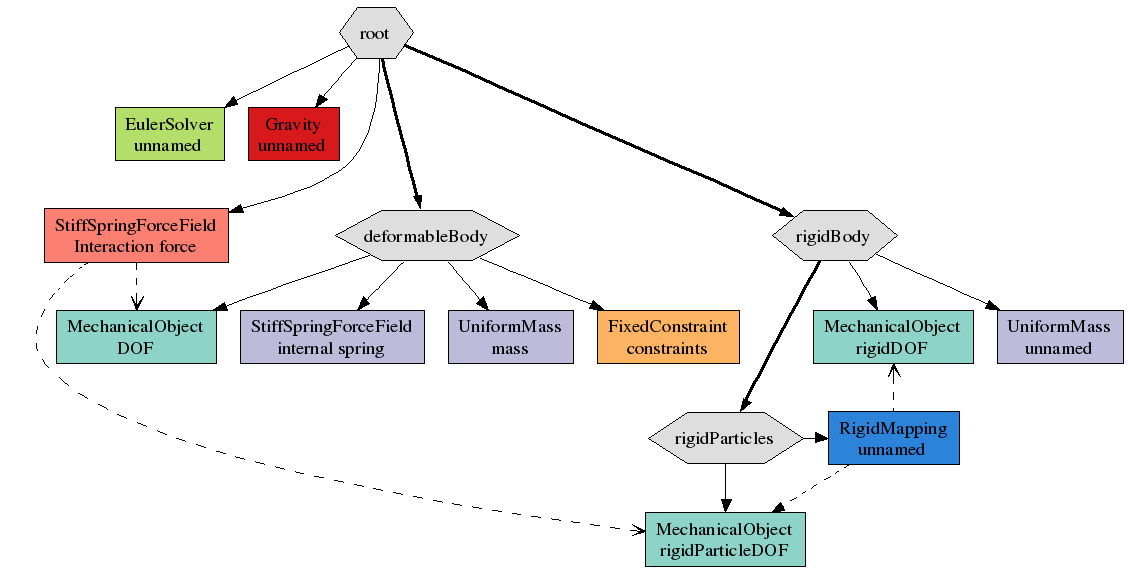
\includegraphics[width=0.9\linewidth]{mixedPendulum.png}
 \caption{A pendulum composed of a rigid body (reference frame and yellow point) attached to an elastic string (green) fixed at one end (pink point). 
 The corresponding scene graph is displayed on the left.}
 \label{fig:mixedPendulum}
\end{figure}
This scene is modeled and simulated in C++ as shown in section~\ref{cpp:hybrid}. 
The corresponding scene graph is shown in figure~\ref{fig:mixedPendulum-graph}. 
Note that the graph in the left of figure~\ref{fig:mixedPendulum} only displays a hierarchical view, while the whole graph includes additional pointers displayed as dashed arrows in figure~\ref{fig:mixedPendulum-graph}.
\begin{figure}
 \centering
 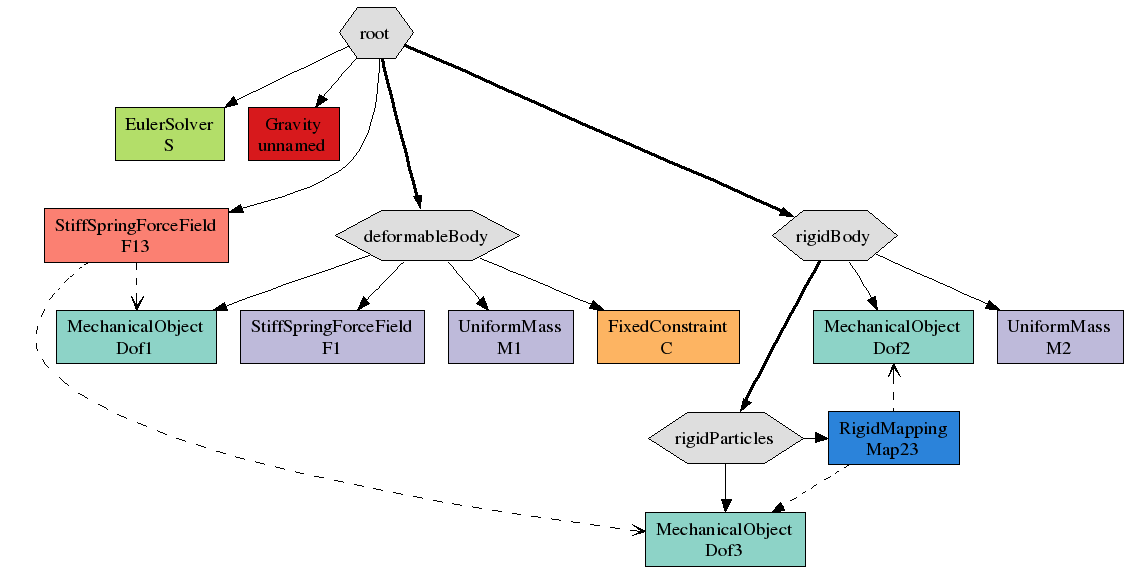
\includegraphics[width=\linewidth]{mixedPendulum-graph}
 \caption{The scene graph of the mixed pendulum. 
 The nodes are displayed as grey hexagons, while the components are displayed as rectangles with colors associated with their types or roles. 
 The bold plain arrows denote node hierarchy, while the thin plain arrows point to the components attached to the nodes, and the dotted arrows denote pointers between components.}
 \label{fig:mixedPendulum-graph}
\end{figure}

The scene is modeled as a tree structure with four nodes:
\begin{itemize}
 \item \texttt{root}
 \item \texttt{deformableBody} corresponds to the elastic string
 \item \texttt{rigidBody} corresponds to the rigid object
 \item \texttt{rigidParticles} corresponds to a set of particles (only one in this case) attached to the rigid body
\end{itemize}
Each node can have children nodes and \textit{components}. 
Each component implements a reduced set of functionalities.


One of the most important type of component is the \texttt{MechanicalObject}, which contains a list of \textit{degrees of freedom} (DOF), i.e. coordinates, velocities, and associated auxiliary vectors such as forces and accelerations.
All the coordinates in a \texttt{MechanicalObject} have the same type, e.g. 3D vectors for particles, or (translation, rotation) pairs for rigid bodies. 
\texttt{MechanicalObject}, like many other \sofa classes, is a generic (C++ template) class instantiated on the types of DOF it stores.
The particle DOFs are drawn as white points, whereas the rigid body DOFs are drawn as red, green, blue reference frame axes.
There can be at most one \texttt{MechanicalObject} attached to a given node. 
This guarantees that all the components attached to the same node process the same types of DOF. 
Consequently, the particles and the rigid body necessarily belong to different nodes.

In this example, the masses are stored in \texttt{UniformMass} components.
The types of their values are related to the types of their associated DOF.
\texttt{UniformMass} is derived from the abstract \texttt{Mass} class, and stores only one value, for the case where all the associated objects have the same mass. 
If necessary, it can replaced by a \texttt{DiagonalMass} instanciated on the same DOF types, for the case where the associated objects have different masses. 
This is an important feature of \sofa: each component can be replaced by another one deriving from the same abstract class and instantiated on the same DOF types. 
This results in a high flexibility.

The \texttt{FixedConstraint} component attached a particle to a fixed point in world space, drawn in pink. 
The constraints act as filters which cancel the forces and displacements applied to their associated particle(s). 
They do not model more complex constraints such as maintaining three points aligned.

The \texttt{StiffSpringForceField} stores a list of springs, each of them modeled by a pair of indices, as well as the standard physical parameters, stiffness, damping and rest length.

The rigid body is connected to the deformable string by a spring.
Since this spring is shared by the two bodies, it is modeled in the \texttt{StiffSpringForceField} attached to a common ancestor, the graph root in this example.
Our springs can only connect particles. 
We thus need to attach a particle to the rigid body. 
Since the particle DOFs types are different from the rigid body DOF types, they have to be stored in another \texttt{MechanicalObject}, called \texttt{rigidParticleDOF} in this example, and attached to a different node.
However, \texttt{rigidParticleDOF} is not a set of independent DOF, since they are fixed in the reference frame of the rigid body. We thus attach it to a child node of the rigid body, and connect it to \texttt{rigidDOF} using a \texttt{RigidMapping}. 
This component stores the coordinates of the particle in the reference frame of the rigid body. 
Its task is to propagate the position, velocity and displacement of the rigid body down to the yellow particle, and conversely, to propagate the forces applied to the particle up to the rigid body.

Mappings are one of the major features of \sofa. 
They allow us to use different geometric models for a given body, e.g. a coarse tetrahedral mesh for viscoelastic internal forces, a set of spheres for collision detection and modeling, and a fine triangular mesh for rendering.

The gravity applied to the scene is modeled in the \texttt{Gravity} component near the root. 
It applies to all the scene, unless locally overloaded by another gravity component inside a branch of the tree.

The abstract component classes are defined in namespace \texttt{core::componentmodel}.

So far, we have discussed the physical model of the scene.
To animate it, we need to solve an \textit{Ordinary Differential Equation} (ODE) in time.
There are plenty of ODE solvers, and \sofa allows the design and the re-use of a wide variety of them.
Here we use a simple explicit Euler method, modeled using an \texttt{EulerSolver} component.
It triggers computations such as force accumulation, acceleration computation and linear operations on state vectors.
More sophisticated solvers are available in \sofa, and can be used by simply replacing the  \texttt{EulerSolver} component by another one, e.g \texttt{RungeKutta4} or \texttt{CGImplicit}.

Other capabilities of \sofa, such as collision detection and response, will be discussed in subsequent sections.

\section{Multi-model objects} \label{sec:multimodel}
An important feature of Sofa is the possibility of using different models of a single physical object. Figure~\ref{fig:liver} shows a scene graph representing a liver, and three different images of it.
The liver exhibits three different geometries for mechanics, rendering and collision.
\begin{figure}
 \centering
 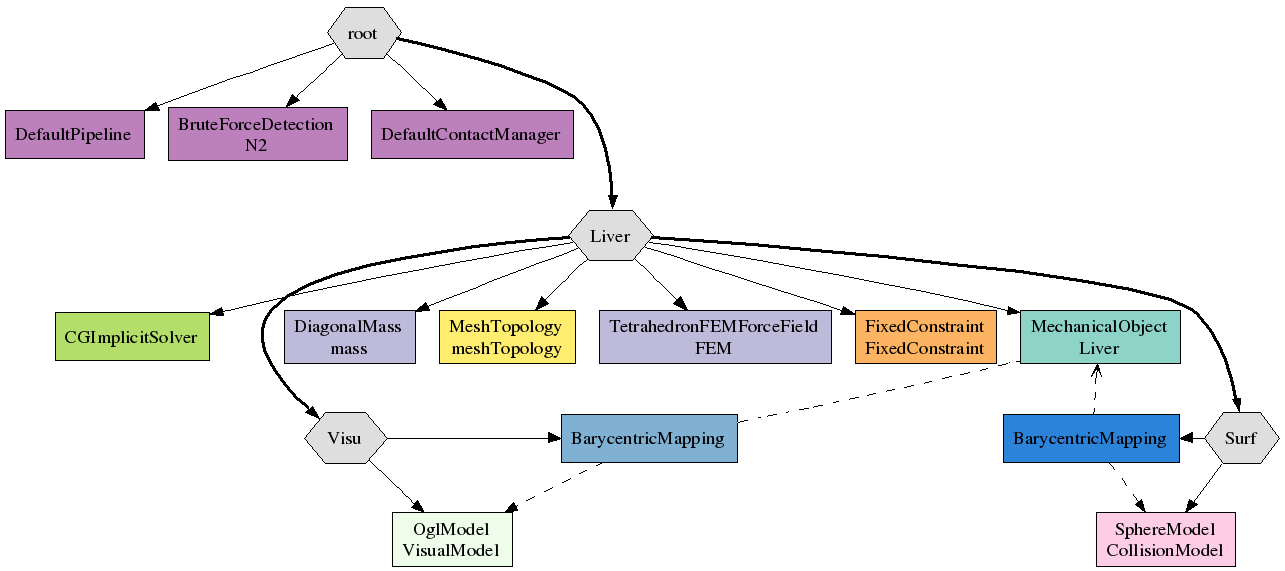
\includegraphics[width=0.95\linewidth]{liver_graph}\\
 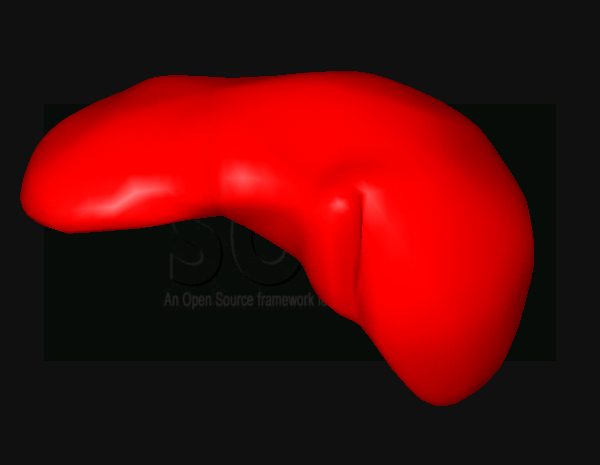
\includegraphics[width=0.3\linewidth]{liver_smooth_visu}
 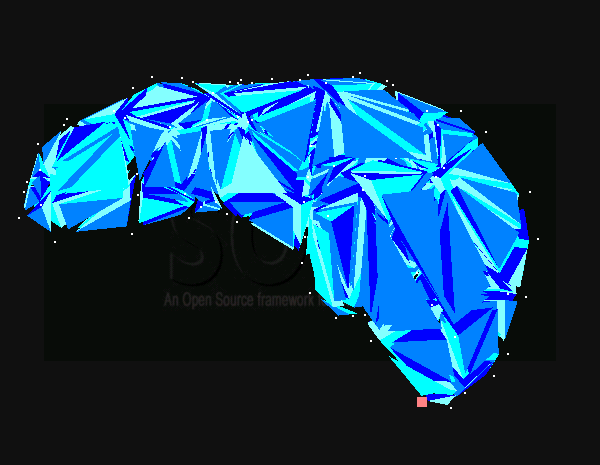
\includegraphics[width=0.3\linewidth]{liver_behavior}
 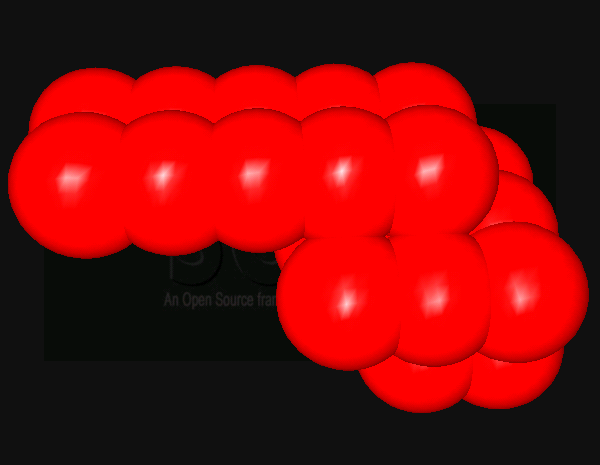
\includegraphics[width=0.3\linewidth]{liver_collision}
 \caption{A liver. Top: scene graph. Bottom: visual model, mechanical model, collision model, respectively.}
 \label{fig:liver}
\end{figure}
The corresponding xml code is given in section~\ref{xml:liver}.
\label{bla:liver}

On top of the scene, collision-related components allow a user to interact with the collision models using rays casted from the mouse pointer and hitting collision models. 
%Collision is discussed in section~\ref{sec:collision}.

The liver is modeled using three nodes, in two levels. 
The parent level contains the mechanical DOFs (particle positions and velocities) in a \texttt{MechanicalObject} component. 
These DOFs are the mechanically independent degrees of freedom of the object, in Lagrange's formalism. 
The node also contains components related to the dynamics of the particles, such as mass and internal forces. 
We call it the \textit{behavior model}.

The two other nodes are in the lower level because during the simulation, their coordinates are totally defined by the coordinates of their parent node. 
Thus, they do not belong to the set of mechanically independent DOFs. 
\emph{Mappings} are used to compute their positions and velocities based on their parent's, using the pointers represented as dashed arrows. 
Mappings are not symmetric. 
The motion of the parent DOFs is mapped to the children DOFs, whereas the motion of the children DOFs is not mapped to their parent. 
This ensures consistency.

The \texttt{VisualModel} has vertices which are used for rendering, along with other rendering data such as a list of polygons, normals, etc. 
The mapping is one-way and the mapped DOFs have no mechanical influence.

The \texttt{SphereModel} class derives from \texttt{MechanicalObject}, with an additional radius value. 
It also derives from \texttt{CollisionModel}, which allows it to be processed by the collision detection and modeling pipeline. 
When contact or mouse interaction forces are applied to the spheres, the forces are propagated bottom-up to their parent DOFs by the mapping. 
This allows the contact forces to be taken into account in the dynamics equations. 
The mapping is thus two-ways and derives from \texttt{MechanicalMapping} instead of \texttt{Mapping}. 
This is why it has a different color in the image of the scene graph.
Again, the mechanical mappings are not symmetric: the forces are propagated from the children to the parents, not the other way round.

Mappings only propagate positions top-down, whereas MechanicalMappings additionally propagate velocities top-down and forces bottom-up.

Mapped models can be designed independently of their parent models, provided that the adequate (mechanical) mapping is available. 
This results in a high flexibility. 
For example, collision spheres can be replaced by collision triangles without changing anything in the behavior model or in the visual model. 
Similarly, other visual models can be used without modifying the behavior and collision models, and different behavior models can be used with the same collision and visual models, as illustrated in figure~\ref{fig:behaviormodels}.

\begin{figure}
 \centering
 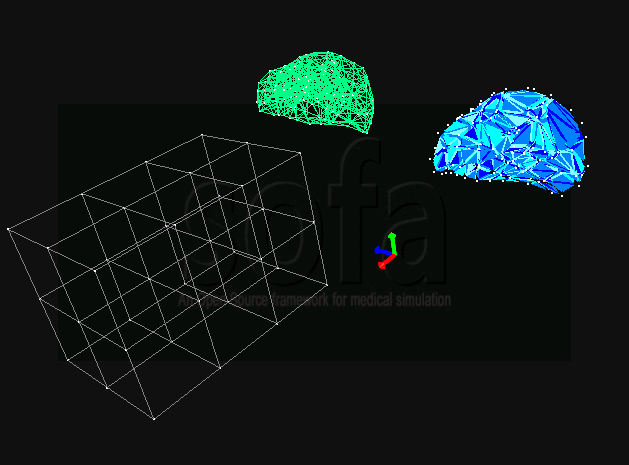
\includegraphics[width=0.4\linewidth]{demoLiverFall1.png}
 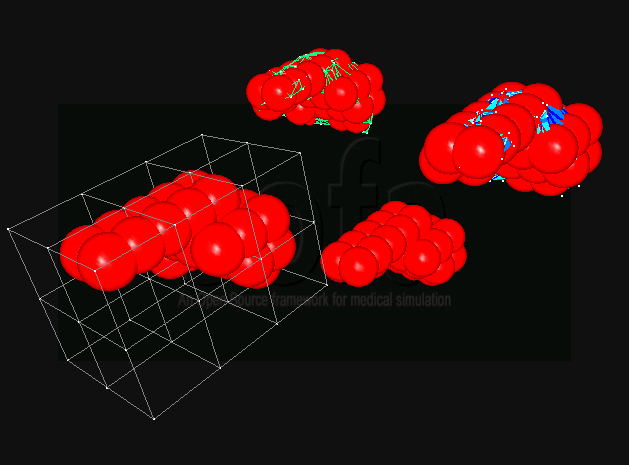
\includegraphics[width=0.4\linewidth]{demoLiverFall2.png}
 % demo.: 1179666x1179666 pixel, 0dpi, infxinf cm, bb=
 \caption{Left: four behavior models (from left to right: deformable grid, springs, rigid, tetrahedral FEM) combined with the same collision model (right).}
 \label{fig:behaviormodels}
\end{figure}


\section{Recursive data processing}
A typical simulation program, controlled by an application such as the Graphics User Interface (GUI), looks like the one given in figure~\ref{pc:animationloop}.
\begin{figure}
\begin{code_cpp}
init();
repeat {
    animate();
    draw();
}
\end{code_cpp}
\caption{Pseudocode for a standard simulation program.}
\label{pc:animationloop}
\end{figure}
In \sofa, each of the simulation methods is implemented as a recursive graph traversal, \texttt{InitVisitor}, \texttt{AnimateVisitor} and \texttt{VisualDrawVisitor}, respectively. 
Visitors are explained in the next section.

\subsection{Visitors}
The data structure is processed using objects called \emph{visitors}.
They recursively traverse the tree structure and call appropriate virtual methods to a subset of components during the \textit{Top-Down Traversal} (TDT), using virtual method \texttt{Visitor::processNodeTopDown}, then during the \textit{Bottom-Up Traversal} (BUT), using virtual method \texttt{Visitor::processNodeBottomUp}.

For example, the \texttt{VisualDrawVisitor} draws the \texttt{VisualModel} components during the TDT, and does nothing during the BUT.
The \texttt{MechanicalComputeForceVisitor} accumulates the forces in the appropriate DOF vectors during the TDT, then propagates the forces to the parent DOFs using the mechanical mappings during the BUT.

When processed by a visitor $a$, a component can fire another visitor $b$ through its associated sub-tree. 
Visitor $a$ can continue once visitor $b$ is finished.
During the TDT, each traversed component decides whether the calling visitor continues, or prunes the sub-tree associated with the component, or terminates.

The components directly access their sibling components only, except for the mappings.
A component traversed by a visitor can indirectly access the data in its associated sub-tree in read-write mode using visitors, whereas data in its parent graph is read-only and only partially accessible using method \texttt{getContext}.
Sibling nodes of the same type can be traversed by visitors in arbitrary order.

The visitors belong to namespace \texttt{simulation::tree}.

\subsection{ODE Solvers}
When an \texttt{AnimateVisitor} traverses a node with an \texttt{OdeSolver} component,
the solver takes the control of its associated subtree and prunes the \texttt{AnimateVisitor}. 
The solver triggers visitors in its associated subtree to perform the standard mechanical computations and integrate time.

The simplest solver is the explicit Euler method, implemented in \texttt{EulerSolver}. 
The algorithm is shown as pseudocode in figure~\ref{pc:expliciteuler}.
\begin{figure}
\begin{code_cpp}
f = 0
accumulateForces(f,x,v);
a = f/M;
a = filter(a);
x += v * dt;
v += a * dt;
\end{code_cpp}
\caption{Pseudocode for explicit Euler integration.}
\label{pc:expliciteuler}
\end{figure}
Net force is computed in the first line.
In the second line, the acceleration is deduced by dividing the force by the mass.
Then the accelerations of the fixed points are canceled.
Finally, position and velocity are updated.

This algorithm can not be directly implemented in \sofa because there are no state vectors x,v,f,a which gather the state values of all the objects in the scene.
The solver processes an arbitrary number of objects, of possibly different types, such as particles and rigid bodies. Each physical object carries its state values and auxiliary vectors in its own \texttt{MechanicalObject} component, which is not directly accessible to the solver.

The solvers represent state vectors as \texttt{MultiVector} objects using symbolic identificators implemented in class \texttt{VecId}.
There are four staticly predefined identificators: \texttt{VecId::position()}, \texttt{VecId::velocity()}, \texttt{VecId::force()} and \texttt{VecId::dx()}.
A \texttt{Multivector} declared by a solver with a given VecId implicitly refers to all the state vectors in the different \texttt{MechanicalObject} components with the same \texttt{VecId} in the solver's subtree.

Vector operations can be remotely triggered by a solver using a visitor of a given type, which defines the operator, and given \texttt{VecId}s, which define the operands.
During the subtree traversal, the operator is applied to the given vectors of the traversed \texttt{MechanicalObject} components.

For example, let us comment the visitors performed by the \texttt{EulerSolver} shown in figure~\ref{fig:mixedPendulum}. Its implementation is in method \texttt{component::odesolver::EulerSolver::solve(double)}.
First, multivectors are declared.

Then method \texttt{core::componentmodel::behavior::OdeSolver::computeForce(VecId)} is called. 
It first fires a \texttt{MechanicalResetForceVisitor} to reset the force vectors of all the \texttt{MechanicalObject} components. 
It then fires a  \texttt{MechanicalComputeForceVisitor}. 
During the TDT, each component derived from \texttt{core::componentmodel::behavior::BaseForceField} computes and accumulates its force in its sibling \texttt{MechanicalObject}. 
In the example shown in figure~\ref{fig:mixedPendulum}, \texttt{F13} adds its contribution to \texttt{Dof1} and \texttt{Dof3}, then \texttt{F1} and \texttt{M1} add their contributions to \texttt{Dof1}, then \texttt{M2} to \texttt{Dof2}. 
Then during the BUT, the mechanical mappings sum up the forces of their chid DOF to their parent DOF, \textit{i.e.}, the force in \texttt{Dof3} to \texttt{Dof2} through \texttt{M23} in the same example.
Note that branches \texttt{deformableBody} and \texttt{rigidBody} can be processed in parallel.
At the end, the force vector in \texttt{Dof1} contains the net force applied to the particles, and the force vector in \texttt{Dof2} contains the net (six-dimensional) force applied to the rigid body.

Then method \texttt{OdeSolver::accFromF(VecId,VecId)} fires a \texttt{MechanicalAccFromFVisitor}. 
Each component derived from \texttt{core::componentmodel::behavior::BaseMass} computes the accelerations corresponding to the forces in its sibling \texttt{MechanicalObject}.

Then method \texttt{OdeSolver::projectResponse} fires a \texttt{MechanicalApplyConstraintsVisitor}. 
All the \texttt{core::componentmodel::behavior::BaseConstraint} components (component \texttt{C} in the example) filter the acceleration vector to maintain some points fixed.

Once the acceleration is computed, multivector methods are used to update the positions and velocities. 
Here again, visitors are used to perform the desired operation in each traversed \texttt{MechanicalObject}.

MultiVector operations are pruned at the first level for efficiency, because the solvers deal with the mechanically independent state variables rather than the mapped variables.
Moreover, the mapped coordinates can not be assumed to vary linearly along with their parent variables.
Applying a \texttt{MechanicalPropagatePositionAndVelocityVisitor} is thus necessary to update the mapped DOFs based on the mechanically independent DOFs.
This visitor is automatically performed after time integration, as one can see in the code of method \\ \texttt{MechanicalIntegrationVisitor::fwdOdeSolver}.
It is also used by some solvers when auxiliary states are needed, as discussed in section~\ref{sec:statevectors}, in order to update the mapped DOFs.

\todo{Call tree of AnimateVisitor, restricted to sofa::core and sofa::simulation::tree}

\todo{Discuss independent and shared solvers}

\section{State vectors} \label{sec:statevectors}
The state vectors contain the coordinates, velocites, and other DOF-related values such as force and acceleration.
They are stored in \texttt{MechanicalObject} components.
This template class can be instanciated on a variety of types to model particles, rigid bodies or other types of bodies.
The template parameter is a \texttt{DataTypes} class which describes data and data containers, such as the the type of coordinates and coordinate derivatives used.
These two types are the same in the case of particles, but they are different in the case of rigid bodies.

Each \texttt{MechanicalObject} can represent a set of physical objects of the same type, such as particles.
The coordinate state vectors are defined by the \texttt{VecCoord} type, while the derivatives (velocity, acceleration, force, small displacement) are defined by the \texttt{VecDeriv} type.
Each \texttt{MechanicalObject} stores two arrays of state vectors, one for coordinates and the other for derivatives, as illustrated in figure~\ref{fig:mechanicalobject}.
\begin{figure}
 \centering
 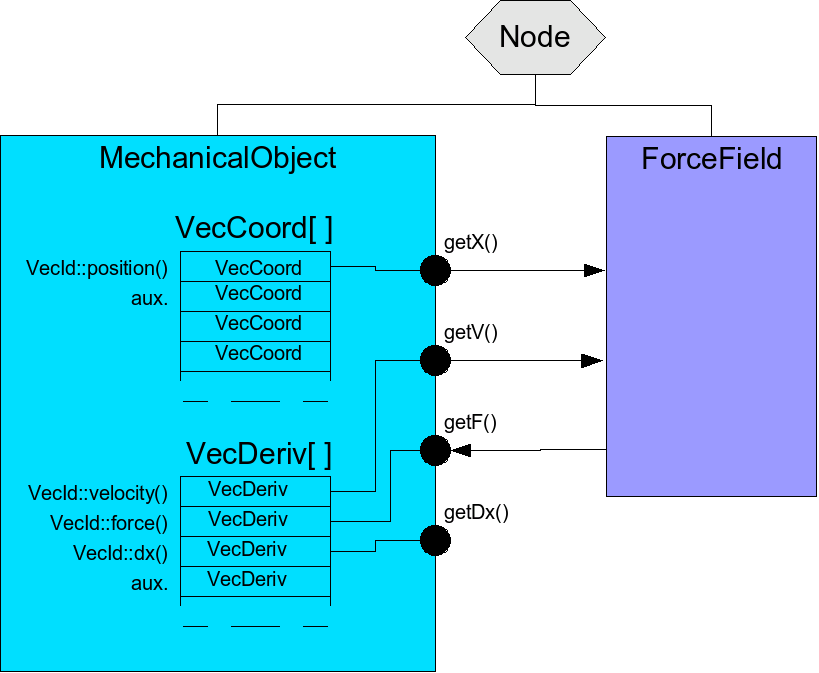
\includegraphics[width=0.45\linewidth]{MechanicalObject1}
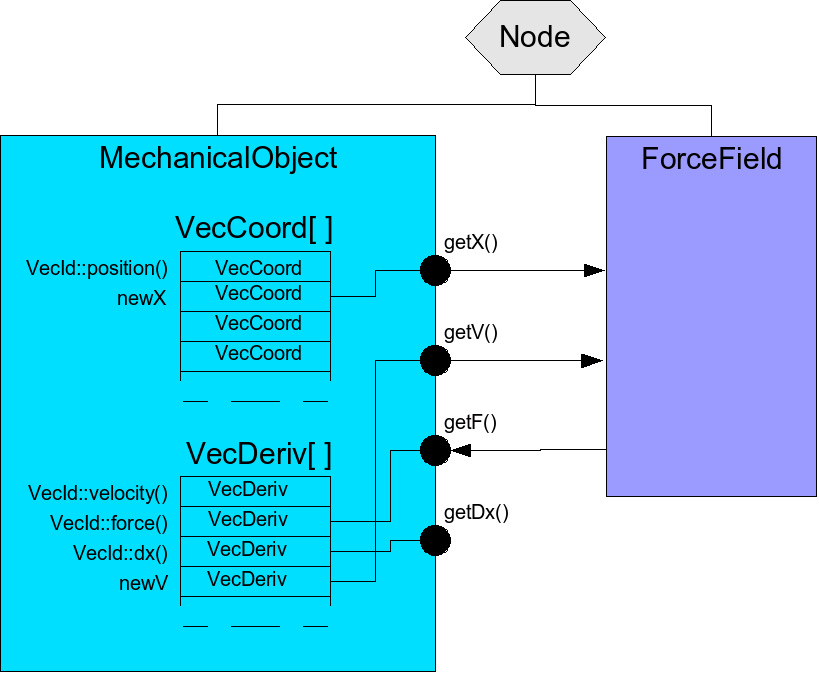
\includegraphics[width=0.45\linewidth]{MechanicalObject2}
  \caption{A \texttt{MechanicalObject} and a component addressing it. Left: using the default state vectors. Right: using auxiliary state vectors.}
 \label{fig:mechanicalobject}
\end{figure}

Auxiliary vectors are necessary for complex solvers, such as \texttt{RungeKutta2Solver}. 
This solver first performs a half-length Euler step, then evaluates the derivative of this new state (called the \emph{midpoint}), and finally uses this derivative to update the initial state over a whole time step.

To compute the forces at the midpoint while keeping the initial state for further use, we use the auxiliary vectors \texttt{newX} and \texttt{newV}.
However, components such as forces and constraints use state vectors, and we have to make sure that they use the right ones.
To ensure consistency and make the use of auxiliary states transparent, the other components get access to the state vectors using methods \texttt{MechanicalObject::getX()}, \texttt{getV()}, \texttt{getF()} and  \texttt{getDx()}.
These methods return pointers to the appropriate vectors, as illustrated in figure~\ref{fig:mechanicalobject}.

Internal  \texttt{MechanicalObject} switches are performed by methods \texttt{MechanicalObject::setX()}, \texttt{setV()}, \texttt{setF()} and  \texttt{setDx()}.
These methods are applied by the visitors which take multivectors as parameters, before they use other components. 
See, for example, method\\ \texttt{MechanicalPropagatePositionAndVelocityVisitor::fwdMechanicalState}.

Note that some constraint-based animation methods require large state vectors and matrices encompassing all the mechanical objects of the scene.
Such methods are currently under development in \sofa, and they are not yet documented.
They use visitors to count the total number of scalar DOFs and to gather them in large state vectors, as well as to build mechanical matrices  such as mass, stiffness, damping and compliance etc.

\subsection{Mechanical groups}
During the simulation, each solver prunes the \texttt{AnimateVisitor} which traverses it and manages its associated subtree by itself using other visitors.
The objects animated by a given solver are called a \emph{mechanical group}.
Each mechanical group corresponds to a subtree in the scene graph.
In the example discussed in section~\ref{sec:commentedExample}, there is one mechanical group because a single solver located near the root manages the whole scene.
However, using separate solvers for different objects can sometimes increase efficiency.
In the example shown in figure~\ref{fig:twoSolvers}, the same deformable body is animated using a \texttt{RungeKutta2Solver} while the rigid body is animated using an \texttt{EulerSolver}.
\begin{figure}
 \centering
 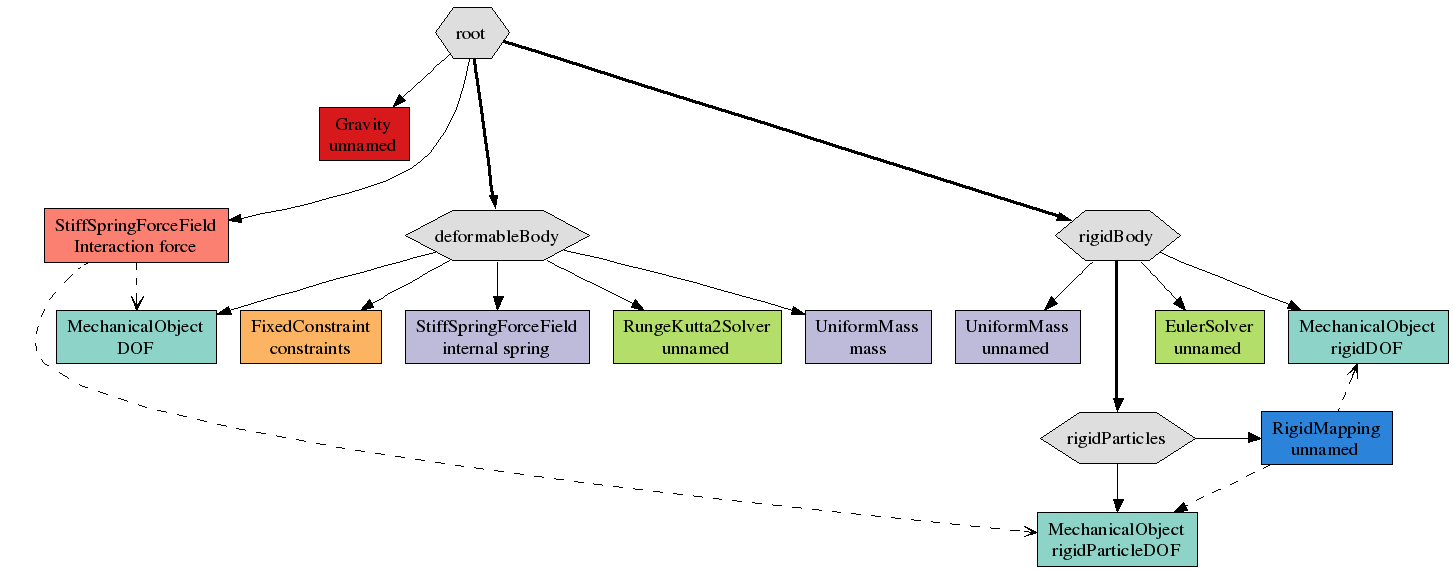
\includegraphics[width=0.95\linewidth]{twoSolvers}
  \caption{A scene graph with objects animated using different ODE solvers.}
 \label{fig:twoSolvers}
\end{figure}


A mechanical group can include interaction forces between elements of the group, and such interaction forces are handled by the solver as expected.
Interaction forces can also occur between objects which do not belong to the same group.
In this case, the interaction force is located at a higher hierarchical level than the objects it applies to, as shown in figure~\ref{fig:twoSolvers}.
It can not be traversed by visitors fired by the solvers.
Its evaluation is performed by the \texttt{AnimateVisitor}, and accumulated as external forces in the associated \texttt{MechanicalObject} components.
Consequently, it acts as a constant constant force during each whole animation step.
In a \texttt{RungeKutta2Solver}, during the force computation at midpoint, its value is the same as at the starting point.
In a \texttt{CGImplicitSolver}, its stiffness is not taken into account, which may introduce instabilities if its actual stiffness is high.

The default collision manager of Sofa circumvents this problem by dynamically gathering the objects in contact in a common mechanical group.

% \section{Mostly used components and methods}
% \subsection{ForceFields}
% \subsection{Constraints}
% \subsection{Masses}
% \subsection{Mappings}
% \subsection{ContextObjects}
%
% \section{Collision detection} \label{sec:collision}
%
%
% \section{Limitations}

% \pagebreak
% \appendix
\section{Code of the examples}
\subsection{The hybrid pendulum}\label{cpp:hybrid}
This is the code of the example commented in section~\ref{sec:commentedExample} :
\includecode{C++}{../applications/tutorials/mixedPendulum/Main.cpp}

\subsection{A liver}\label{xml:liver}
This is the XML code of the liver discussed in section~\ref{sec:multimodel} page~\pageref{bla:liver} :
\includecode{XML}{../scenes/liver.scn}

% \chapter{Animation in \sofa}\label{chapter:as}
This section shows how the material presented in chapter \ref{chapter:pba} is implemented in \sofa. A class diagram of the mechanical core is presented in appendix \ref{sec:umlmeca}.
\section{Particles}
\subsection{Simple example}
Here we simulate two particles subject to gravity. An introduction to particle dynamics is given in section \ref{sec:particles}. 
Figure \ref{fig:singleParticleCollaboration} shows the collaboration diagram and the code used to model a set of particles subject to gravity. The code is available in project {\tt doc/src\_examples/example1}.


\begin{figure}[htp]
\begin{center} \begin{tabular}{cc}
\begin{minipage}[b]{6cm}
	\includegraphics*[width=6cm]{fig/singleParticleCollaboration.eps}  
	%\input{fig/singleParticleCollaboration.tex} 
\end{minipage}
 &
\begin{minipage}[b]{9cm} 
\begin{code_cpp}
#include "Sofa/Components/Scene.h"
#include "Sofa/Components/MassObject.h"
#include "Sofa/Components/EulerSolver.h"
#include "Sofa/GUI/FLTK/Main.h"

using namespace Sofa::Components;
using namespace Sofa::Core;
using namespace Sofa::GUI::FLTK;
typedef Sofa::Components::Common::Vec3Types MyTypes;
typedef MyTypes::Deriv Vec3;
        
int main(int argc, char** argv) 
{
    Scene* scene = new Scene;
    scene->setDt(0.04);
    
    MechanicalGroup* group = new MechanicalGroup;
    scene->addBehaviorModel(group);
    group->setSolver( new EulerSolver );
    
    MassObject<MyTypes>* particles = new MassObject<MyTypes>;
    group->addObject(particles);
    scene->addVisualModel(particles);                 
    particles->setGravity( Vec3( 0,-1,0 ) );
    particles->addMass( Vec3(2,0,0), Vec3(0,0,0), 1 ); 
    particles->addMass( Vec3(3,0,0), Vec3(0,0,0), 1 );


    scene->init();
    MainLoop(argv[0]);
    return 0;
}
\end{code_cpp}
\end{minipage}
\end{tabular}
\end{center}
\label{fig:singleParticleCollaboration} 
\caption{Collaboration diagram and code for the animation of free particles.}
\end{figure}


%
% \chapter{Extending \sofa}\label{chapter:es}

This chapter presents how different types of classes can be added to \sofa{} to implement new behaviors.

\section{Adding a new DynamicObject}

A DynamicObject is responsible for implementing the behavior of a given type of body. It contains the degrees of freedoms (\textit{DOFs}) of the body (within the MechanicalObject class), as well as its mass (i.e. how the body moves given an applied force).

To add a new DynamicObject in \sofa, the following steps are required:

\begin{enumerate}
\item Specify the type of its DOFs in a \textcode{DataTypes} class.
\item Create the \textcode{DynamicObject} derived class implementing the behaviors of the body, or instantiate an existing class with you \textit{DataTypes} class if already available.
\item Create a method to create an instance of the body given an XML node.
\item Register the new DynamicObject in the \textcode{Sofa::Components::XML::DynamicNode::Factory} factory.
\item Create a XML scene file containing a DynamicModel with the \textit{type} of our class.
\item Have fun!
\end{enumerate}

If the new class will only be created procedurally, then only the first two steps are required.

We will now detail these steps using the example of an object containing a set of one-dimensional particles.

The code corresponding to this example is available in the following files:
\begin{description}
\item[Sofa/doc/src\_examples/example3/MassObject1d.h]~\\
 Declaration of MassObject1d.
\item[Sofa/doc/src\_examples/example3/MassObject1d.cpp]~\\
 Creation from XML and registration in the Factory
\item[Sofa/doc/src\_examples/example3/Main.cpp]~\\
 Main program
\item[Sofa/doc/src\_examples/example3/test1.scn]~\\
 Test scene file
\end{description}

\subsection{Specification of the Degrees of Freedom}\label{sec:DOF}

The data types used by the body are specified in a class containing the following definitions:

\begin{description}
\item[Coord]~\\
 Type of DOFs.
\item[Deriv]~\\
 Type of derivatives (velocity, forces, displacements).
\item[VecCoord]~\\
 Container of DOFs.
\item[VecDeriv]~\\
 Container of derivatives.
\item[void set(Coord\& c, double x, double y, double z)]~\\
 Utility method to set the value of a point.
\item[void add(Coord\& c, double x, double y, double z)]~\\
 Utility method to add a value to a point (for applyTranslation).

\end{description}

In our example, we can use double as the type of DOFs and std::vector as containers:

\begin{code_cpp}
class Vec1dTypes
{
public:
  typedef double Coord;
  typedef double Deriv;
  typedef std::vector<Coord> VecCoord;
  typedef std::vector<Deriv> VecDeriv;
  
  /// Here we only use the first coordinate
  static void set(Coord& c, double x, double /*y*/, double /*z*/)
  {
    c = x;
  }
  
  static void add(Coord& c, double x, double /*y*/, double /*z*/)
  {
    c += x;
  }
};
\end{code_cpp}

\subsection{Body Behaviors Implementation}

In \sofa{} a DynamicObject does not implement the time integration algorithm, which is handled by an separate Solver. Instead, it implements basic operations, such as compute forces, combine several vectors, etc. Of these operations, most are only dependant on the types of DOFs, or are computed through external classes (ForceFields for instance). Only 3 operations related to the mass remain to be implemented by DynamicObject subclasses:

\begin{description}
\item[computeForce] must be modified to add gravity ( $\ve f = \ve f + \ma M \ve g$ ).
\item[accFromF] must be implemented to convert forces to accelerations ( $\ve a = \ma M^{-1} \ve f$ ).
\item[addMDx] must be implemented to multiply a given displacement by the mass ( $ \ve r = \ve r + \ma M \ve dx$ ).
\end{description}

In our example, a class \textcode{MassObject} already exists to handle object represented as a set of particles. So we just need to instantiate it to the type of DOFs we want to use:

\begin{code_cpp}
typedef MassObject<Vec1dTypes> MassObject1d;
\end{code_cpp}

As a reference, here is how MassObject implements the 3 operations mentioned earlier:

\begin{code_cpp}
template <class DataTypes>
void MassObject<DataTypes>::addMDx(VecDeriv* res, VecDeriv* dx)
{
  for( unsigned i=0; i<dx->size(); ++i )
    (*res)[i] += (*dx)[i] * masses[i].mass;
}


template <class DataTypes>
void MassObject<DataTypes>::accFromF(VecDeriv* a, VecDeriv* f)
{
  a->resize(f->size());
  for( unsigned i=0; i<f->size(); ++i )
    (*a)[i] = (*f)[i] / masses[i].mass;
}


template <class DataTypes>
void MassObject<DataTypes>::computeForce(VecDeriv* result)
{
  Inherit::computeForce(result);
  // Add Gravity
  for (unsigned int i=0;i<result->size();i++)
  {
    (*result)[i]+=gravity*masses[i].mass;
  }
}
\end{code_cpp}

\subsection{Instantiation from XML}

\sofa{} implements a mechanism to load a scene from a XML file using a two step process:

\begin{enumerate}
\item The XML file is parsed and converted to a tree of Node class.
\item Each node use a Factory to instantiate the described object.
\end{enumerate}

A DynamicObject is described by a \textcode{Sofa::Components::XML::DynamicNode}. It contains the type of the class to instantiate, as well as a set of string attributes. To build our DynamicObject from this description we need a function to construct and configure a new instance given the pointer to the XML::DynamicNode. This can either be a constructor in our class, or an external function with the following prototype:
\begin{code_cpp}
namespace Sofa { namespace Components { namespace Common {
void create(MyDynamicObject*& obj, XML::Node<Sofa::Abstract::DynamicModel>* arg);
} } }
\end{code_cpp}
where \textcode{MyDynamicObject} is the name of our new class.

\textbf{Note:} the inclusion in the \textcode{Sofa::Components::Common} namespace is necessary for the Factory class to find our function. If anyone find a better design removing this requirement please tell me!

Typically, the object will either be constructed from attributes given in the XML node, or using an external description file.

Our 1D particles example is simple enough not to require an external file. We can implement a creation function as follow:

\begin{code_cpp}
/// Read a vector of scalars from a string.
void readVec1(std::vector<double>& vec, const char* str)
{
  vec.clear();
  if (str==NULL) return;
  const char* str2 = NULL;
  for(;;)
  {
    double v = strtod(str,(char**)&str2);
    std::cout << v << std::endl;
    if (str2==str) break;
    str = str2;
    vec.push_back(v);
  }
}

namespace Sofa { namespace Components { namespace Common {
/// Construct a MassObject1d object from a XML node.
void create(MassObject1d*& obj, XML::Node<Sofa::Abstract::DynamicModel>* arg)
{
        obj = new MassObject1d();
  obj->clear();
  std::vector<double> mass;
  std::vector<double> pos;
  std::vector<double> vel;
  std::vector<double> fixed;
  readVec1(mass,arg->getAttribute("mass"));
  readVec1(pos,arg->getAttribute("position"));
  readVec1(vel,arg->getAttribute("velocity"));
  readVec1(fixed,arg->getAttribute("fixed"));
  if (arg->getAttribute("gravity"))
  {
    obj->setGravity(atof(arg->getAttribute("gravity")));
  }
  unsigned int maxsize = mass.size();
  if (pos.size()>maxsize) maxsize = pos.size();
  if (vel.size()>maxsize) maxsize = vel.size();
  double defaultmass = (mass.empty()?1.0:*mass.rbegin());
  while (mass.size()<maxsize)
    mass.push_back(defaultmass);
  double defaultpos = 0;
  if (!pos.empty()) defaultpos = *pos.rbegin();
  while (pos.size()<maxsize)
    pos.push_back(defaultpos);
  double defaultvel = 0;
  if (!vel.empty()) defaultvel = *vel.rbegin();
  while (vel.size()<maxsize)
    vel.push_back(defaultvel);
  for (unsigned int i=0;i<maxsize;i++)
  {
    obj->addMass(pos[i], vel[i], mass[i], 0.0,
      (std::find(fixed.begin(), fixed.end(), (double)i)!=fixed.end()));
  }
} } } }
\end{code_cpp}

Note that this function is quite long, as it construct vectors of values (masses, positions, velocities) from strings. For simpler cases, where only a filename is required for instance, generic creation functions are provided:
\begin{code_cpp}
namespace Sofa { namespace Components { namespace Common {
/// Construct a MassObject1d object from a XML node using an external file.
void create(MassObject1d*& obj, XML::Node<Sofa::Abstract::DynamicModel>* arg)
{
  XML::createFromFilename(obj, arg);
} } } }
\end{code_cpp}
However it is then necessary to implement the external file loading method.

\subsection{Factory Registration}

Once all functionalities are implemented, it is necessary to register the new class in the \textcode{Sofa::Components::XML::DynamicNode::Factory} factory in order for \sofa{} to know about it. This requires adding the following "magic" line:

\begin{code_cpp}
Creator< XML::DynamicNode::Factory, MassObject<Vec1dTypes> >
  MassObject1dClass("MassObject1d");
\end{code_cpp}

This command will register our class to the Factory during the initialization of the program. For this to work we must still ensure our code is linked in the final binary. To do this we must add the following line in the .cpp file containing the Creator command:
\begin{code_cpp}
\end{code_cpp}
and then add a corresponding line in a .cpp file used during the execution of the program (such as the file containing the main() function, or in Sofa/Components/init.cpp if the new class is integrated in \sofa{}):
\begin{code_cpp}
SOFA_INIT_CLASS(MassObject1d)
\end{code_cpp}
This last step is required to work around portability issues, and might be removed if a better solution is found.

When the given type name is used in an XML file, the Factory will now be able to construct our custom DynamicObject.

\subsection{Testing}

Our new class can now be loaded by writing a small XML file:

\begin{code_xml}
<Scene dt="0.005" showBehaviorModels="1" showCollisionModels="1" showMappings="1" showForceFields="1">
	<Group>
		<Solver type="RungeKutta4"/>
		<DynamicModel type="MassObject1d" name="M1" position="0 1 2 3 4 5" fixed="5" gravity="-9.8"/>
	</Group>
</Scene>
\end{code_xml}

To run it, go to \textcode{Sofa/doc/src\_examples/example3} and execute
\begin{code_bash}
./run test1.scn
\end{code_bash}

\begin{figure}
\centering
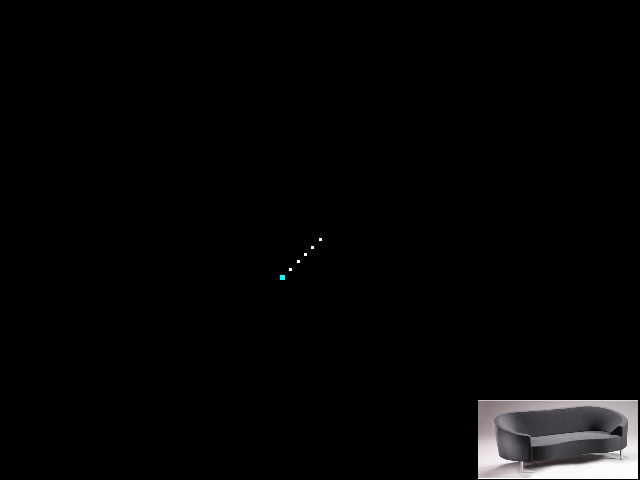
\includegraphics[width=0.5\linewidth]{fig/mass1d}
\caption{Test scene with 6 1D particles.}
\end{figure}

\section{Adding a new Mapping}

Many existing objects in \sofa{} expect to work with 3D particles. To be able to use them with our 1D particles, we can create a MechanicalMapping which will convert information between the two representations.

Adding a new Mapping in \sofa{} requires the following steps:

\begin{enumerate}
\item Create the \textit{Mapping} or \textit{MechanicalMapping} derived class computing the mapping from the input model to the output, and accumulating forces back for MechanicalMappings.
\item Create a method to create an instance of the mapping given an XML node.
\item Register the new mapping in the Sofa::Components::XML::MappingNode::Factory factory.
\item Create a XML scene file containing a Mapping with the \textit{type} of our class.
\item Have more fun!
\end{enumerate}

We will now detail these steps using the 1D to 3D mechanical mapping example.
The code for this mapping is available in the \textcode{Sofa/doc/src\_examples/example3/LinearMapping.cpp} file.

\subsection{Mapping Implementation}

A MechanicalMapping is used in the scene to link two MechanicalObjects, an input model and an output model. Positions, velocities and displacements are propagated from the input model to the output, and forces are accumulated in the other direction. This can be implemented by overloading 3 methods:

\begin{description}
\item[apply] compute output positions from input ones
\item[applyJ] compute output derivatives (velocity of displacement) from input ones
\item[applyJT] accumulate back output forces (or df) into input ones
\end{description}

If the mapping is linear these operations can be expressed in terms of the mapping matrix $\ma J$: apply and applyJ are equivalent to ${\mathbf {out}} = \ma J {\mathbf {in}}$, and applyJT is equivalent to $ {\mathbf {in}} += \ma {J^{t}} {\mathbf {out}} $.

A scene in \sofa{} can contain mechanical models with different types of degrees of freedoms (see section~\ref{sec:DOF}). The mapping can either be generic relatively to the types used in the input and output models, or requires them to use specific types. The first solution requires the mapping implementation to be declared as a template of the type of DOFs, while the second solution requires implementing a "standard" class.

For our example, we will create a non-templated mapping for simplicity, although a templated version would be very similar.

\begin{code_cpp}
class LineMapping : public Sofa::Core::MechanicalMapping< Sofa::Core::MechanicalObject<Vec1dTypes>, Sofa::Core::MechanicalObject<Vec3dTypes> >
{
public:
  // Simplified notation for all involved classes
  typedef Sofa::Core::MechanicalMapping< Sofa::Core::MechanicalObject<Vec1dTypes>, Sofa::Core::MechanicalObject<Vec3dTypes> > BaseMapping;
  typedef BaseMapping::In In;
  typedef BaseMapping::Out Out;
  typedef Out::VecCoord VecCoord;
  typedef Out::VecDeriv VecDeriv;
  typedef Out::Coord Coord;
  typedef Out::Deriv Deriv;

  Coord p0; ///< Origin of the 3D line
  Deriv dx; ///< Direction of the 3D line
  
  LineMapping(In* from, Out* to, const std::string& /*name*/)
  : BaseMapping(from, to), p0(0,0,0), dx(1,0,0)
  {
  }
  
  void apply( Out::VecCoord& out, const In::VecCoord& in )
  {
    out.resize(in.size());
    for(unsigned int i=0;i<out.size();i++)
      out[i] = p0+dx*in[i];
  }
  
  void applyJ( Out::VecDeriv& out, const In::VecDeriv& in )
  {
    out.resize(in.size());
    for(unsigned int i=0;i<out.size();i++)
      out[i] = dx*in[i];
  }
  
  void applyJT( In::VecDeriv& out, const Out::VecDeriv& in )
  {
    for(unsigned int i=0;i<out.size();i++)
      out[i] += dx*in[i];
  }
};
\end{code_cpp}

\subsection{Instantiation from XML and Registration in Factory}

This process is identical to the corresponding steps in the DynamicObject case, except that the XML Node to use is XML::MappingNode instead of XML::DynamicNode.

In our example, the additional code required for this step is:
\begin{code_cpp}

namespace Sofa { namespace Components { namespace Common {

void create(LineMapping*& obj, XML::Node<Sofa::Core::BasicMapping>* arg)
{
  XML::createWith2Objects< LineMapping, LineMapping::In, LineMapping::Out>(obj, arg);
  if (obj!=NULL)
  {
    obj->p0[0] = atof(arg->getAttribute("x0","0"));
    obj->p0[1] = atof(arg->getAttribute("y0","0"));
    obj->p0[2] = atof(arg->getAttribute("z0","0"));
    obj->dx[0] = atof(arg->getAttribute("dx","1"));
    obj->dx[1] = atof(arg->getAttribute("dy","0"));
    obj->dx[2] = atof(arg->getAttribute("dz","0"));
  }
} } } }

Creator< XML::MappingNode::Factory, LineMapping > LineMappingClass("LineMapping", true);
\end{code_cpp}

Note the true argument in the Creator command. It means that other classes with the same type name are authorized in the Factory, implementing the same mapping for other datatypes for instance.

\subsection{Testing}

Our new class can now be used to add a 3D spring force field to our 1D masses by writing a small XML file:

\begin{code_xml}
<Scene dt="0.005" showBehaviorModels="1" showCollisionModels="1" showMappings="1" showForceFields="1">
	<Group>
		<Solver type="RungeKutta4"/>
		<DynamicModel type="MassObject1d" name="M1" position="0 1 2 3 4 5" fixed="5" gravity="-9.8">
		<MechanicalModel type="Vec3d" name="Points">
		<ForceField type="StiffSpringForceField" filename="test2.xs3"/>
		</MechanicalModel>
		<Mapping type="LineMapping" input="@." output="@Points" />
		</DynamicModel>
	</Group>
</Scene>
\end{code_xml}

To run it, go to \textcode{Sofa/doc/src\_examples/example3} and execute
\begin{code_bash}
./run test2.scn
\end{code_bash}

The same mapping can also be used to attach a collision model:

\begin{code_xml}
<Scene dt="0.005" showBehaviorModels="1" showCollisionModels="1" showMappings="1" showForceFields="1">
	<CollisionPipeline>
		<CollisionDetection name="N2" type="BruteForce" />
		<Contact name="Response" response="penality" />
		<CollisionGroup name="Group" />
	</CollisionPipeline>
	<Group>
		<Solver type="RungeKutta4"/>
		<DynamicModel type="MassObject1d" name="M1" position="0 1 2 3 4 5" fixed="5" gravity="-9.8">
		<MechanicalModel type="Vec3d" name="Points">
		<ForceField type="StiffSpringForceField" filename="test2.xs3"/>
		</MechanicalModel>
		<Mapping type="LineMapping" input="@." output="@Points" />
		<CollisionModel type="Sphere" name="Spheres" filename="test3.sph"/>
		<Mapping type="LineMapping" input="@." output="@Spheres" />
		</DynamicModel>
	</Group>
</Scene>
\end{code_xml}

To run it, go to \textcode{Sofa/doc/src\_examples/example3} and execute
\begin{code_bash}
./run test3.scn
\end{code_bash}

\begin{figure}
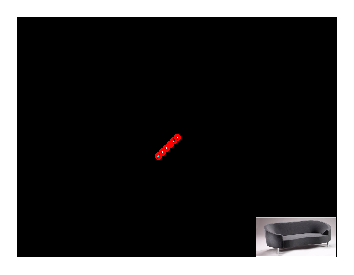
\includegraphics[width=0.5\linewidth]{fig/mass1d-collision1}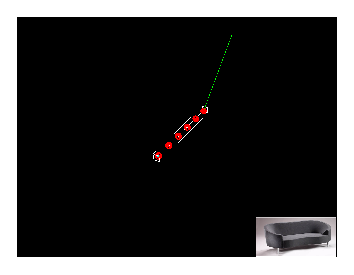
\includegraphics[width=0.5\linewidth]{fig/mass1d-collision2}
\caption{Collisions with 1D particles used to interact with the mouse.}\label{fig:mass1d-collision}
\end{figure}

\begin{figure}
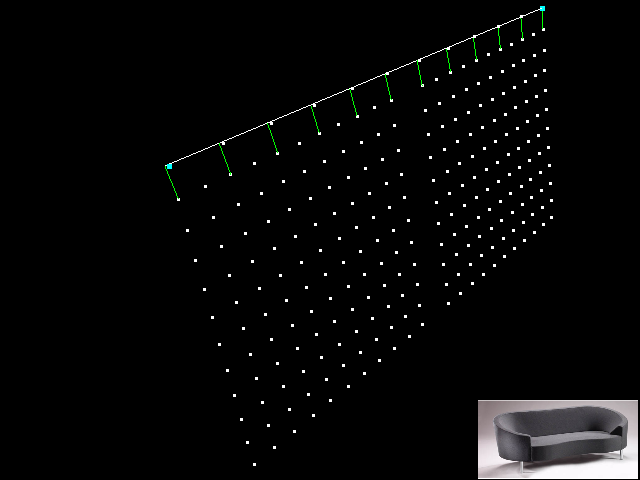
\includegraphics[width=0.5\linewidth]{fig/mass1d-curtain1}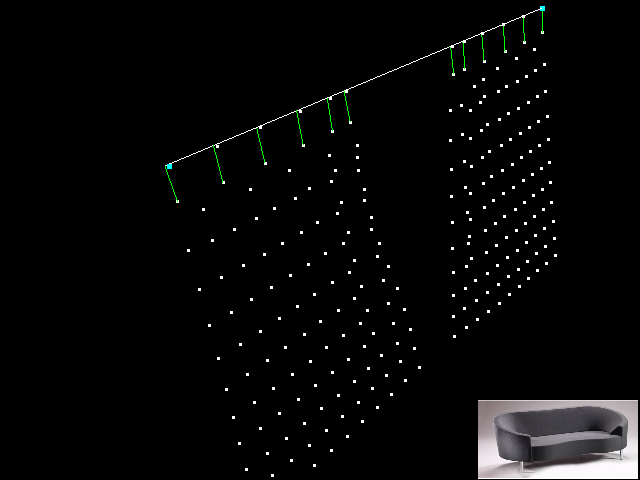
\includegraphics[width=0.5\linewidth]{fig/mass1d-curtain2}\\
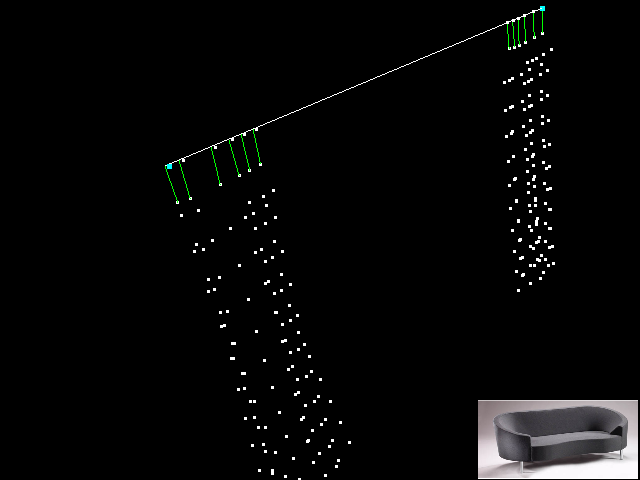
\includegraphics[width=0.5\linewidth]{fig/mass1d-curtain3}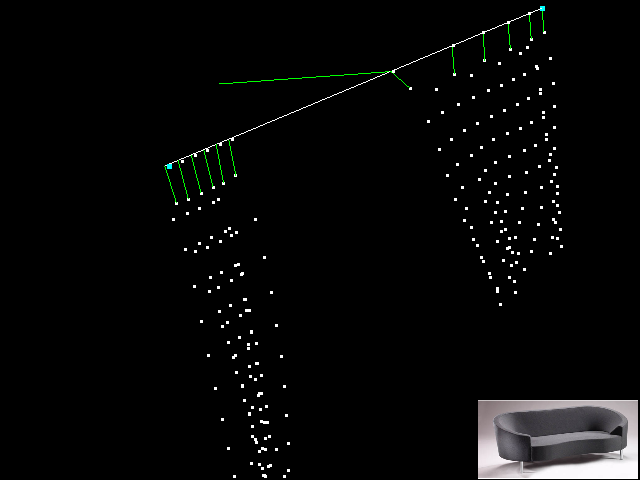
\includegraphics[width=0.5\linewidth]{fig/mass1d-curtain4}%
\caption{1D and 3D particles linked by springs to simulate curtains.}\label{fig:mass1d-curtain}
\end{figure}

You can now pick the particles with the mouse by pressing the shift key and left mouse button, as seen in figure~\ref{fig:mass1d-collision}.

The main advantage of our mapping is that we can combine 1D and 3D particles in the same simulation with forces such as springs applied between them. This is demonstrated in the \texttt{test4.scn} scene, as seen in figure~\ref{fig:mass1d-curtain}.

\section{Non-Linear Mapping}

Mappings are not limited to linear computations. Non-linear mappings can be computed exactly in the apply method, and a local linear approximation can be used for the applyJ and applyJT methods.

For instance, our 1D particles can be mapped to a circle instead of a line. The code for this mapping is available in the
\textcode{Sofa/doc/src\_examples/example3/CircleMapping.cpp} file. It uses the following computations :

\begin{description}
\item[apply] $ \ve x_{out} = \ve{p_0} + \ve{r_x} cos( \ve x_{in} ) + \ve{r_y} sin( \ve x_{in} ) $
\item[applyJ] $ \ve v_{out} = \frac{\delta \ve x_{out}}{\delta \ve x_{in}} \ve v_{in} = ( - \ve{r_x} sin ( \ve x_{in} ) + \ve{r_y} cos ( \ve x_{in} ) ) \ve v_{in} $
\item[applyJT] $ \ve f_{in} = \frac{\delta \ve x_{out}}{\delta \ve x_{in}} \ve f_{out} $ and $ \frac{\delta \ve f_{in}}{\delta \ve x_{in}} = \frac{\delta \ve x_{out}}{\delta \ve x_{in}^2} \ve f_{out} + \frac{\delta \ve x_{out}}{\delta \ve x_{in}} \frac{\delta \ve f_{out}}{\delta \ve x_{out}} $
\end{description}

Note that if we use a local linear approximation, $ \frac{\delta \ve x_{out}}{\delta \ve x_{in}^2} = 0 $ so applyJT is the same for f and df.

\begin{code_cpp}
class CircleMapping : public Sofa::Core::MechanicalMapping< Sofa::Core::MechanicalObject<Vec1dTypes>, Sofa::Core::MechanicalObject<Vec3dTypes> >
{
public:
  // Simplified notation for all involved classes
  typedef Sofa::Core::MechanicalMapping< Sofa::Core::MechanicalObject<Vec1dTypes>, Sofa::Core::MechanicalObject<Vec3dTypes> > BaseMapping;
  typedef BaseMapping::In In;
  typedef BaseMapping::Out Out;
  typedef Out::VecCoord VecCoord;
  typedef Out::VecDeriv VecDeriv;
  typedef Out::Coord Coord;
  typedef Out::Deriv Deriv;

  Coord p0; ///< Origin of the circle
  Deriv rx, ry; ///< Radius of the circle
  
  std::vector<Deriv> dx;
  
  CircleMapping(In* from, Out* to, const std::string& /*name*/)
  : BaseMapping(from, to), p0(0,0,0), rx(1,0,0), ry(0,0,1)
  {
  }
  
  void apply( Out::VecCoord& out, const In::VecCoord& in )
  {
    out.resize(in.size());
    dx.resize(in.size());
    for(unsigned int i=0;i<out.size();i++)
    {
	  double c = cos(in[i]);
	  double s = sin(in[i]);
      out[i] = p0+rx*c+ry*s;
	  dx[i] = rx*(-s)+ry*c;
    }
  }
  
  void applyJ( Out::VecDeriv& out, const In::VecDeriv& in )
  {
    out.resize(in.size());
    for(unsigned int i=0;i<out.size();i++)
      out[i] = dx[i]*in[i];
  }
  
  void applyJT( In::VecDeriv& out, const Out::VecDeriv& in )
  {
    for(unsigned int i=0;i<out.size();i++)
      out[i] += dx[i]*in[i];
  }
};
\end{code_cpp}

To run it, go to \textcode{Sofa/doc/src\_examples/example3} and execute
\begin{code_bash}
./run test5.scn
\end{code_bash}

The result is visible in figure~\ref{fig:mass1d-circle}.

\begin{figure}
\centering
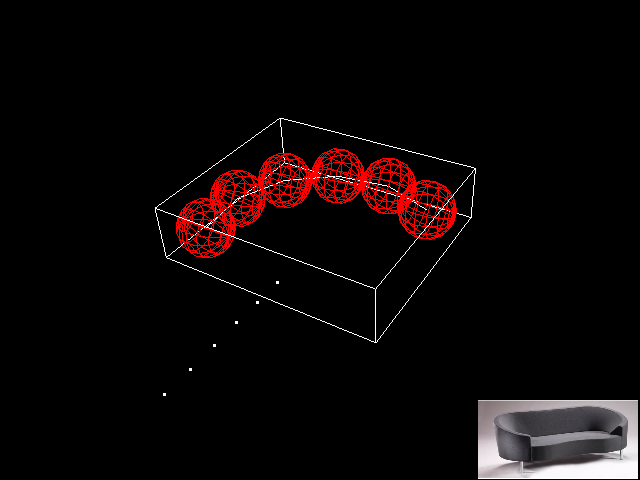
\includegraphics[width=0.5\linewidth]{fig/mass1d-circle1}
\caption{1D particles mapped to a circle.}\label{fig:mass1d-circle}
\end{figure}

\section{Adding a new ForceField}

A ForceField is used to apply forces to mechanical objects in the scene. Its basic role is to compute a force vector $\ve f$ associated with a set of DOFs, given their position $\ve x$ and velocity $\ve v$. To support implicit integration schemes, it must also compute the force derivative $\ve{df}$ given a displacement $\ve {dx}$.

Adding a new ForceField in \sofa{} requires the following steps:

\begin{enumerate}
\item Create the ForceField derived class.
\item Create a method to create an instance of the force field given an XML node.
\item Register the new force field in the \textcode{Sofa::Components::XML::ForceFieldNode::Factory} factory.
\item Create a XML scene file containing a ForceField with the \textit{type} of our class.
\item Have even more fun!
\end{enumerate}

We will now detail these steps implementing \textit{Lennard-Jones} fluid forces. It is a simple force field adding a force between any pair of particles based on a potential related to their distance $d$:\\
$potential = \dfrac{a}{d^\alpha} - \dfrac{b}{d^\beta}$\\
$f = - grad(potential) = ( a \alpha d^{-\alpha-1} - b \beta d^{-\beta-1} ) \ve u$\\
where $\ve u$ is the unit vector between the two particles. This force field has the property to force particles to stay within a certain distance of each other, and is negligible for particles far away from each other, allowing to use a cutoff distance.

Computing the Lennard-Jones forces requires $5$ parameters: $a$, $b$, $\alpha$, $\beta$, and the cutoff distance $d_{max}$. As they are not all meaningful, we will instead allow the user to specify the prefered distance $d_0$ where $f = 0$, as well as the potential value $p_0$ at this point, which controls the force magnitude. The cutoff distance $d_{max}$ will be initialized as $2 d_0$ by default, and we will use $\alpha=6$ and $\beta=12$. The $a$ and $b$ parameters can then be computed as follow:\\
$$
\left\{\begin{array}{rl}
a \alpha d_0^{-\alpha-1} - b \beta d_0^{-\beta-1} &= 0 \\
a d_0^{-\alpha} - b d_0^{-\beta} &= p_0 \\
\end{array}\right\}
\Longrightarrow
\left\{\begin{array}{rl}
b &= a \frac{\alpha}{\beta} d_0^{\beta-\alpha} \\
a d_0^{-\alpha} - a \frac{\alpha}{\beta} d_0^{-\alpha} &= p_0 \\
\end{array}\right\}
\Longrightarrow
\left\{\begin{array}{rl}
a &= \dfrac{p_0 d_0^\alpha}{1 - \frac{\alpha}{\beta}} \\
b &= \dfrac{p_0 d_0^\beta}{\frac{\beta}{\alpha} - 1} \\
\end{array}\right\}
$$

The code for this force field is available in the
\textcode{Sofa/doc/src\_examples/example4/LennardJonesForceField.\{h,inl,cpp\}} files.

\subsection{ForceField Implementation}

A ForceField is attached to a MechanicalObject in the scene. It is implemented by overloading 2 methods:

\begin{description}
\item[addForce] compute force given the position and velocity in the MechanicalObject
\item[addDForce] compute derived force from the displacement in the MechanicalObject
\end{description}

For small or nearly constant forces, the addDForce method can be ignored. For other cases it uses a linear approximation, as it will be used in the inner loop.

The implementation of a force field is dependant on the type of the DOFs to which it applies. For our example, we will create a templated version for genericity, although a non-templated version could also be used if you prefer.

The class declaration is:

\begin{code_cpp}
template<class DataTypes>
class LennardJonesForceField : public Sofa::Core::ForceField, public Sofa::Abstract::VisualModel
{
public:
	typedef Sofa::Core::ForceField Inherit;
	typedef typename DataTypes::VecCoord VecCoord;
	typedef typename DataTypes::VecDeriv VecDeriv;
	typedef typename DataTypes::Coord Coord;
	typedef typename DataTypes::Deriv Deriv;
	typedef typename Coord::value_type Real;
	
protected:
	Sofa::Core::MechanicalModel<DataTypes>* object;
	
	Real a,b,alpha,beta,dmax,fmax;
	Real d0,p0;

	struct DForce
	{
		unsigned int a,b;
		Real df;
	};
	
	std::vector<DForce> dforces;
	
public:
	LennardJonesForceField(Sofa::Core::MechanicalModel<DataTypes>* object, const std::string& /*name*/="")
	: object(object), a(1), b(1), alpha(6), beta(12), dmax(2), fmax(1), d0(1), p0(1)
	{
	}
	
	void setAlpha(Real v) { alpha = v; }
	void setBeta(Real v) { beta = v; }
	void setFMax(Real v) { fmax = v; }
	void setDMax(Real v) { dmax = v; }
	void setD0(Real v) { d0 = v; }
	void setP0(Real v) { p0 = v; }

	virtual void init();
	
	virtual void addForce();
	
	virtual void addDForce();
	
	// -- VisualModel interface
	void draw();
	void initTextures() { }
	void update() { }
};
\end{code_cpp}

The class implementation is:

\begin{code_cpp}
template<class DataTypes>
void LennardJonesForceField<DataTypes>::init()
{
    a = (p0 * (Real)pow(d0,alpha)) / (1-alpha/beta);
    b = (p0 * (Real)pow(d0,beta)) / (beta/alpha-1);
}

template<class DataTypes>
void LennardJonesForceField<DataTypes>::addForce()
{
	Real dmax2 = dmax*dmax;
	VecDeriv& f1 = *this->object->getF();
	VecCoord& p1 = *this->object->getX();
	this->dforces.clear();
	f1.resize(p1.size());
	for (unsigned int ib=1; ib<p1.size(); ib++)
	{
		const Coord pb = p1[ib];
		for (unsigned int ia=0; ia<ib; ia++)
		{
			const Coord pa = p1[ia];
			const Deriv u = pb-pa;
			const Real d2 = u.norm2();
			if (d2 >= dmax2) continue;
			const Real d = (Real)sqrt(d2);
			const Real fa = a*alpha*(Real)pow(d,-alpha-1);
			const Real fb = b*beta*(Real)pow(d,-beta-1);
			Real forceIntensity = fa - fb;
			//std::cout << ia<<"-"<<ib<<" d="<<d<<" f="<<forceIntensity<<std::endl;
			DForce df;
			df.a = ia;
			df.b = ib;
			if (forceIntensity > fmax)
			{
			    forceIntensity = fmax;
			    df.df = 0;
			}
			else
			{
			    df.df = ((-alpha-1)*fa - (-beta-1)*fb)/(d*d2);
			}
			this->dforces.push_back(df);
			const Deriv force = u*(forceIntensity/d);
			f1[ia]+=force;
			f1[ib]-=force;
		}
	}
}

template<class DataTypes>
void LennardJonesForceField<DataTypes>::addDForce()
{
	VecDeriv& f1  = *this->object->getF();
	VecCoord& p1 = *this->object->getX();
	VecDeriv& dx1 = *this->object->getDx();
	f1.resize(dx1.size());
	for (unsigned int i=0; i<this->dforces.size(); i++)
	{
		const DForce& df = this->dforces[i];
		const unsigned int ia = df.a;
		const unsigned int ib = df.b;
		const Deriv u = p1[ib]-p1[ia];
		const Deriv du = dx1[ib]-dx1[ia];
		const Deriv dforce = u * (df.df * (du*u)); 
		f1[ia] += dforce;
		f1[ib] -= dforce;
	}
}

template<class DataTypes>
void LennardJonesForceField<DataTypes>::draw()
{
	if (!Sofa::Components::Scene::getInstance()->getShowForceFields()) return;
	VecCoord& p1 = *this->object->getX();
	glDisable(GL_LIGHTING);
	glColor4f(0,0,1,1);
	glBegin(GL_LINES);
	for (unsigned int i=0; i<this->dforces.size(); i++)
	{
		const DForce& df = this->dforces[i];
		const unsigned int ia = df.a;
		const unsigned int ib = df.b;
		glVertex3d(p1[ia][0],p1[ia][1],p1[ia][2]);
		glVertex3d(p1[ib][0],p1[ib][1],p1[ib][2]);
	}
	glEnd();
}
\end{code_cpp}

\subsection{Instantiation from XML and Registration in Factory}

This process is identical to the corresponding steps in the DynamicObject and Mapping cases, except that the XML Node to use is XML::ForceFieldNode.

In our example, the additional code required for this step is:
\begin{code_cpp}

namespace Sofa { namespace Components { namespace Common {

template<class DataTypes>
void create(LennardJonesForceField<DataTypes>*& obj, XML::Node<Sofa::Core::ForceField>* arg)
{
  XML::createWithParent< LennardJonesForceField<DataTypes>, MechanicalModel<DataTypes> >(obj, arg);
  if (obj!=NULL)
  {
    if (arg->getAttribute("alpha"))  obj->setAlpha(atof(arg->getAttribute("alpha")));
    if (arg->getAttribute("beta"))  obj->setBeta(atof(arg->getAttribute("beta")));
    if (arg->getAttribute("fmax"))  obj->setFMax(atof(arg->getAttribute("fmax")));
    if (arg->getAttribute("dmax"))  obj->setDMax(atof(arg->getAttribute("dmax")));
    else if (arg->getAttribute("d0"))  obj->setDMax(2*atof(arg->getAttribute("d0")));
    if (arg->getAttribute("d0"))  obj->setD0(atof(arg->getAttribute("d0")));
    if (arg->getAttribute("p0"))  obj->setP0(atof(arg->getAttribute("p0")));
  }
} } } }

// Each instance of our class must be compiled
template class LennardJonesForceField<Vec3fTypes>;
template class LennardJonesForceField<Vec3dTypes>;

// And registered in the Factory
Creator< XML::ForceFieldNode::Factory, LennardJonesForceField<Vec3fTypes> > LennardJonesForceField3fClass("LennardJones", true);
Creator< XML::ForceFieldNode::Factory, LennardJonesForceField<Vec3dTypes> > LennardJonesForceField3dClass("LennardJones", true);
\end{code_cpp}

As our implementation is templated, the create method is also templated, and several Creator must be used, one for each template instantiation we support.

\subsection{Testing}

This new force field can be used to simulate a very simple fluid by initializing a set of particles and applying the Lennard-Jones forces to them.

\begin{code_xml}
<Scene dt="0.005" showBehaviorModels="1" showCollisionModels="1" showMappings="1" showForceFields="1">
	<Group>
		<Solver type="CGImplicit"/>
		<DynamicModel type="MassObject" name="M1" gravity="0 -10 0" mass="0.5">
		<!-- A topology is used here just to set initial particles positions. It is a bad idea because this object has no real topology, but it works... -->
		<Topology type="RegularGrid" nx="8" ny="6" nz="10" xmin="-9" xmax="5" ymin="-8" ymax="2" zmin="-9" zmax="9" />
		<ForceField type="LennardJones" alpha="8" beta="9" p0="-50" d0="1" dmax="4" fmax="1" />
		<!-- The following force fields handle collisions with walls and an inclined floor -->
		<ForceField type="PlaneForceField" normal="1 0 0" d="-10"/>
		<ForceField type="PlaneForceField" normal="-1 0 0" d="-10"/>
		<ForceField type="PlaneForceField" normal="0.1 1 0" d="-10"/>
		<ForceField type="PlaneForceField" normal="0 0 1" d="-10"/>
		<ForceField type="PlaneForceField" normal="0 0 -1" d="-10"/>
		</DynamicModel>
	</Group>
</Scene>
\end{code_xml}

To run it, go to \textcode{Sofa/doc/src\_examples/example4} and execute
\begin{code_bash}
./run test1.scn
\end{code_bash}

\begin{figure}
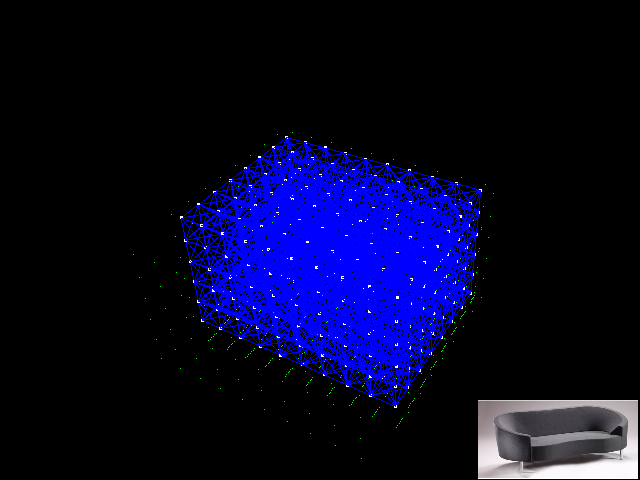
\includegraphics[width=0.33\linewidth]{fig/fluid1-00}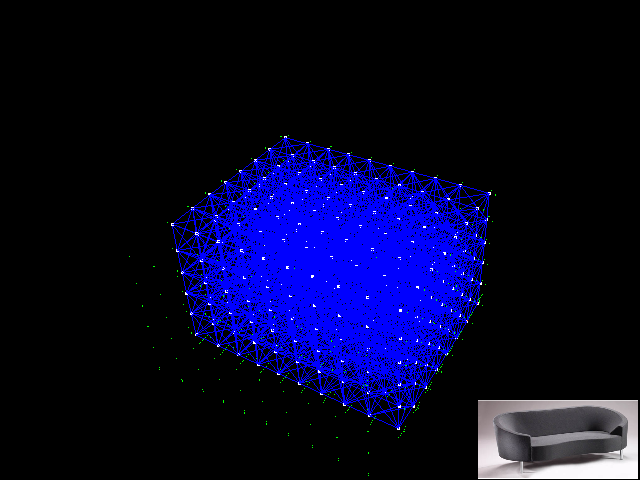
\includegraphics[width=0.33\linewidth]{fig/fluid1-01}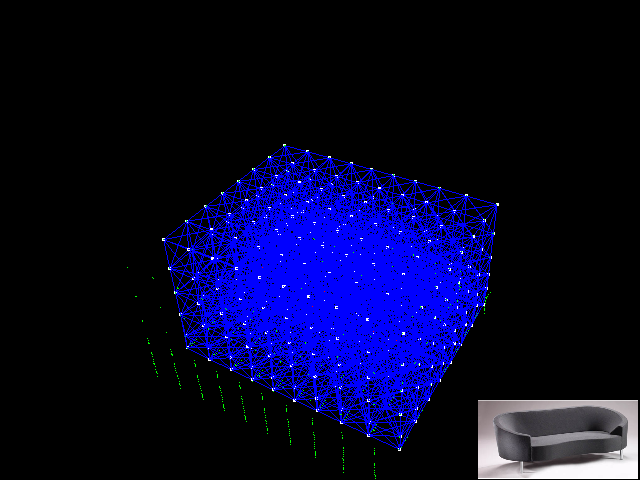
\includegraphics[width=0.33\linewidth]{fig/fluid1-02}\\
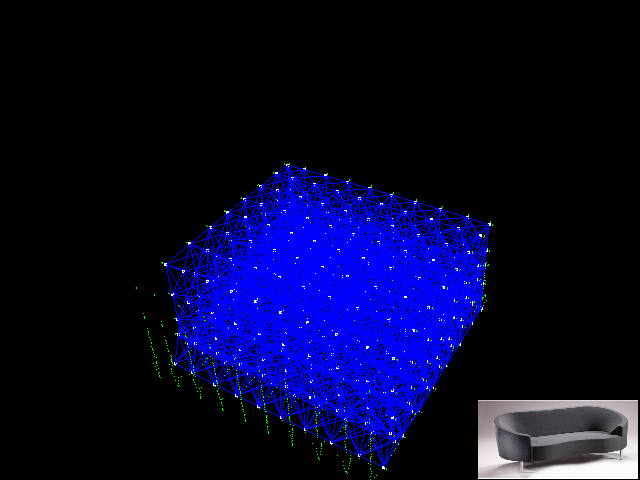
\includegraphics[width=0.33\linewidth]{fig/fluid1-03}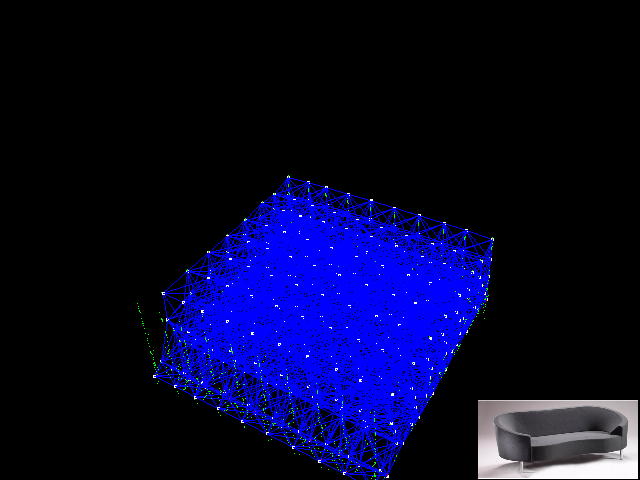
\includegraphics[width=0.33\linewidth]{fig/fluid1-04}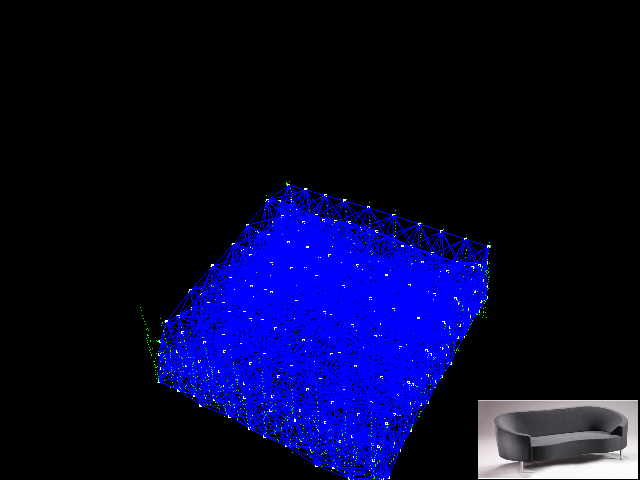
\includegraphics[width=0.33\linewidth]{fig/fluid1-05}\\
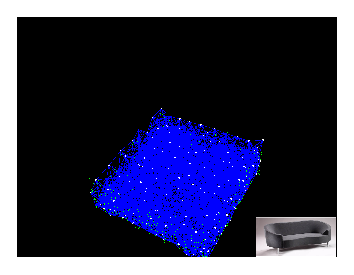
\includegraphics[width=0.33\linewidth]{fig/fluid1-06}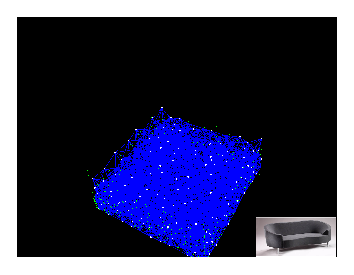
\includegraphics[width=0.33\linewidth]{fig/fluid1-07}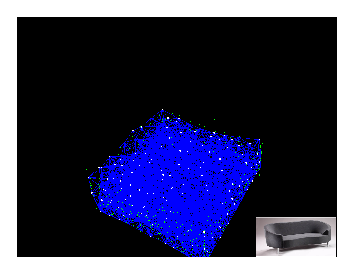
\includegraphics[width=0.33\linewidth]{fig/fluid1-08}\\
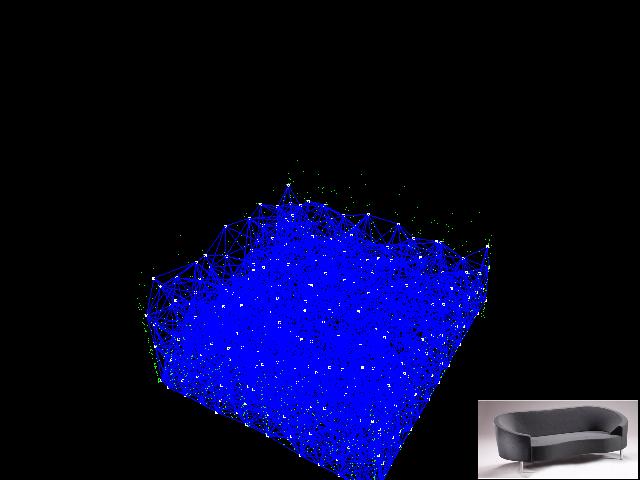
\includegraphics[width=0.33\linewidth]{fig/fluid1-09}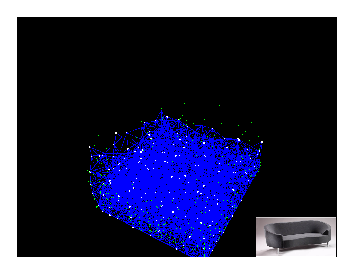
\includegraphics[width=0.33\linewidth]{fig/fluid1-10}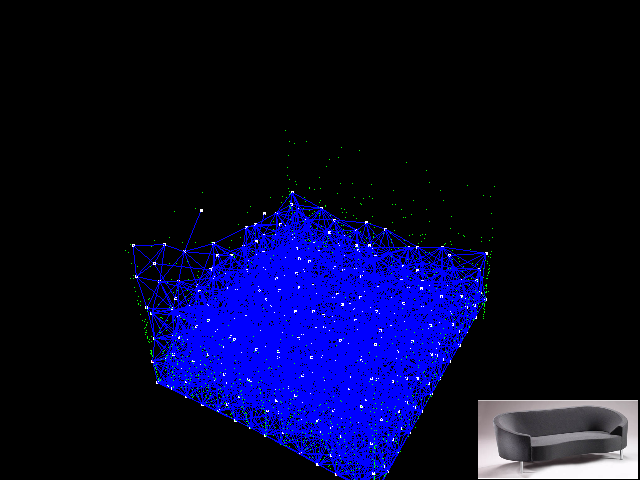
\includegraphics[width=0.33\linewidth]{fig/fluid1-11}
\caption{Fluid animation.}\label{fig:fluid1}
\end{figure}

The resulting animation is shown in figure~\ref{fig:fluid1}.

%
% \chapter{Physically-based animation} \label{chapter:pba}
\section{Particles} \label{sec:particles}
\subsection{Basic equation}
A particle is a moving point with a mass. Generally the mass is a constant over time while its position and velocity can vary. We therefore consider the mass $ m $ (in $ kg $) as an attribute while its position $ x $ (in $ m $) and its velocity $ v $ (in $m.s^{-1}$) are its state variables. 
Particles obey Newton's law: 
\begin{equation} \label{eq:newton}
ma = \Sigma f
\end{equation} 
where $a$ is the particle's acceleration (in $m.s^{-2}$). This defines the Ordinary Differential Equation (ODE) $a(t) = f(x,v,t)$. Physically-based animation requires us to repeatedly solve it over the interval $[t,t+dt]$ and redisplay.

From equation \ref{eq:newton} we can deduce $a=1/m\;\Sigma f$ and integrate time over a time step dt, and so on. The simplest integration method is Euler's explicit scheme:
\begin{eqnarray}
v(t+dt) &=& v(t)+a(t)dt \nonumber \\
x(t+dt) &=& x(t)+v(t)dt \label{eq:expliciteuler}
\end{eqnarray}

Particles can live in any k-dimensional space $\Re^k$, where state variables and forces are k-dimensional vectors of scalar values. The dynamics equation \ref{eq:newton} applies to each scalar value.
When considering $n$ particles the equations can be conveniently written in matrix form:
\begin{eqnarray*}
\ma M \ve a &=& \ve f\\
\ve a &=& \ma M^{-1} \ve f
\end{eqnarray*}
where \ma M is a diagonal matrix of dimension $kn\times kn$ , \ve a and \ve f are vectors of dimension $kn$ gathering all the scalar components associated with each particle.

Numerical integration can generate instabilities leading to the divergence of the simulated system. To avoid this, one solution is to decrease the time step. The other solution is to use an implicit integration scheme, which takes into account the variation of the forces during the time step. The simplest one is the implicit Euler's method which applies a step based on the forces at the end of the time step instead of the beginning. Equation \ref{eq:expliciteuler} becomes:
\begin{eqnarray}
v(t+dt) &=& v(t)+a(t+dt)dt \nonumber\\
x(t+dt) &=& x(t)+v(t+dt)dt \label{eq:impliciteuler}
\end{eqnarray}
Since $a(t+dt)$ is unknown we have to solve an equation.
If we write $v(t+dt) = v(t)+\Delta v$ the matrix form equation to solve is:
\begin{equation}
\label{eq:matimplicit}
\left( \ma M + dt \ma D + dt^2 \ma K \right) \ve{\Delta v} = dt \left( \ve f(t) + \ma D \ve{v}(t) \right) 
\end{equation}
where the damping matrix $\ma D = \delta \ve f/\delta \ve v$ encodes the variation of force given a variation of velocity, and the stiffness matrix $\ma K = \delta \ve f/\delta \ve p$ encodes the variation of force given a variation of position.

\subsection{Forces}
The forces are responsible for the accelerations of the bodies. Their physical unit is the Newton ($N=kg.m.s^{-2}$).
Here we briefly review the most commonly used forces.

\subsubsection{Weight}
A uniform gravitational field $g$ (in $m.s^{-2}$) applies a force 
\begin{equation} \label{eq:gravity}
f = mg
\end{equation} 
to each particle where $m$ is the mass of the particle.

\subsubsection{Linear damping}
Damping transforms kinetic energy to heat by applying a force opposed to the velocity. It tends to slow down the objects. Linear damping is proportional to the velocity, thus 
\begin{equation}\label{eq:lineardamping}
f=-\nu v
\end{equation}
where $v$ is the velocity of the particle and $\nu$ a positive scalar (in $kg.s^{-1}$).

\subsubsection{Air damping}
Air damping is proportional to the square of the velocity of the body with respect to the air:
\begin{equation}
f = -\rho S_u C_u v^2 u 
\end{equation}
where $\rho$ is the volumic mass the air ($kg.m^{-3}$), $v$ the velocity of the object, $u$ a no-dimensional unit vector in the direction of the velocity, $S$ the area ($m^2$) of the object projected along $u$, and $C_u$ a no-dimensional coefficient associated with the shape of the object and the direction $u$.

\subsubsection{Linear springs}
A springs applies an elastic force between two points. It is modeled using its rest length $l_0$ (in $m$) and its stiffness $k$ (in $N.m^{-1}$). 
Let $i$ and $j$ be the indices of points linked by a given spring. 
The force applied by a linear spring to point $i$ is given by:
\begin{equation}
\label{eq:spring}
f_i = k( l-l_0 ) u
\end{equation}
where $l=\|x_j - x_i\|$ is the distance between the points and $u$ a unit vector pointing from point $i$ to point $j$. The force $f_j$ applied to point $j$ is the opposite: $f_j = -f_i$. Nonlinear springs can be used to model more complex behaviors.

\subsubsection{Linear damped springs}
Damping forces are commonly associated with springs in order to dissipate energy. They are opposed to the relative velocity of the points. They are typically modeled using a coefficient $\nu$ (in $kg.s^{-1}$).
The force applied by a linear damped spring to point $i$ is given by:
\begin{equation}
\label{eq:dampedspring}
f_i = \left( k( l-l_0 ) + \nu v_{ij} \right) u
\end{equation}
where $v_{ij} = (v_j-v_i).u$ is the relative velocity of the particles along direction $u$.

\subsubsection{Finite elements}
Finite elements is a powerful paradigm for modeling continuous material. At our level, we can see them as springs acting on more than two points simultaneously. For example, a tetrahedral finite element acts on the four vertices of a tetrahedron and allows a more effective control of stiffness and volume than using springs.


%===========================================================================================

\section{Solids}
A solid is a moving reference frame with a mass matrix. In two dimensions it has three degrees of freedom (DOFs), two translations and one rotation, while in three dimensions it has six DOFs, three translations and three independent rotation values. The remainder of this document focuses on three dimensions.

\subsection{Orientation}
There are different ways of modeling orientation ot one frame with respect to another in three dimensions, each of them with advantages and drawbacks:
\begin{itemize}
\item matrices directly define the axes of the solid with respect to a reference frame. They allow fast projections from one frame to another but they contain nine dependent entries and they can not be set up intuitively;
\item Euler angles are compact (three parameters) and intuitive but they have singularities and they can not be easily combined;
 \item (axis, angle) pairs are more intuitive and more compact (four parameters) than matrices but they do not allow projections and combinations;
\item quaternions are compact (four parameters) and allow easy projections and combinations, but they are not easy to set up intuitively.
\end{itemize}

\subsubsection{Orientation matrices}
Orientations matrices are $3\times 3$ matrices, each column gathering the coordinates of one axis of the rotated frame with respect to the reference frame. Each column is thus a unit vector orthogonal to the others. This creates six relations among the nine parameters, leaving three independent DOFs.

\subsubsection{Euler angles}
Euler angles model a sequence of three rotations along three pairwise-independent directions. For example, the following matrix product represents a rotation $\alpha$ along axis $x$ followed by a rotation $\beta$ along rotated axis $y$ followed by a rotation $\gamma$ along the twice rotated axis $z$.
%\begin{equation}\label{eq:angles euler}
$$
\left(\begin{array}{ccc}
1 & 0 & 0 \\
0 & \cos\alpha & -\sin\alpha \\
0 & \sin\alpha &  \cos\alpha
\end{array}\right)
\left(\begin{array}{ccc}
\sin\beta & 0 &  \cos\beta\\
0 & 1 & 0 \\
\cos\beta & 0 & -\sin\beta
\end{array}\right)
\left(\begin{array}{ccc}
\cos\gamma & -\sin\gamma & 0\\
\sin\gamma & \cos\gamma & 0\\
0 & 0 & 1\\
\end{array}\right)
$$
%\end{equation}
Alternatively, this can be seen as a rotation  $\gamma$ along axis $z$ followed by a rotation $\beta$ along the fixed axis $y$ followed by a rotation $\alpha$ along the fixed axis $x$. An example of singularity is the fact that in this system, rotation $(\pi,\pi,0)$ is equivalent with rotation $(0,0,\pi)$. Another example is the fact that rotation $(\alpha,\pi /2, \gamma)$ is equivalent with rotation $(0,\pi /2, \alpha+\gamma)$ for any $\alpha$ and $\gamma$ (this loss of one DOF is called \emph{gimbal lock}).

\subsubsection{Axis, angle}
The rotation $\theta$ along an axis defined by a unit vector $n$ has the following matrix:
$$
\rot{\theta}{u} = \mat{I} + \sin\theta\oppvec{n} + (1-\cos\theta)\oppvec{n}^2
$$
where matrix $\oppvec{n}$  is the vector product matrix operator: 
%\begin{equation}\label{eq:oppvec}
$$
\oppvec{n} = \left(\begin{array}{ccc}
0 & -n_z & n_y \\
n_z & 0 & -n_x \\
-n_y & n_x & 0
\end{array}\right)
$$
%\end{equation}
It is possible to convert a matrix back to (axis, angle) by noticing that  $\trace{\mat R}=1+2\cos\theta$ et que $\mat R -\transp{\mat R} = 2\sin\theta\oppvec{n}$

\subsubsection{Quaternions}
Quaternions are an extension of complex numbers: $ \bm q = w + x\bm i + y \bm j + z \bm k = (w,\vect v)$.\\
w is the real part, \vect v the imagianry part.
Properties of \bm i, \bm j, \bm k:
$$
\begin{array}{l}
  \bm i^2 = \bm j^2 = \bm k^2 = -1\\
  \bm{ij}=\bm k,\;\bm{ji} = -\bm k\\
  \bm{jk}=\bm i,\;\bm{kj} = -\bm i\\
  \bm{ki}=\bm j,\;\bm{ik} = -\bm j\\
\end{array}
$$
A 3d vector is a pure imaginary quaternion:
$$
\bm p = (0,x,y,z)
$$
Product of quaternions (not commutative):
$$
\bm{q_1q_2} = (w_1w_2 - \bm v_1.\bm v_2, \; w_1\bm v_2 + w_2\bm v_1 + \bm v_1 \wedge \bm v_2)
$$
Conjugate quaternion:
$$
\begin{array}{l}
  \bm{\bar q} = w - x\bm i - y \bm j - z \bm k\\
  \bm{q\bar q} = w^2 + x^2 + y^2 + z^2
\end{array}
$$
Unit quaternions used to model rotations:
$$
\bm{q\bar q} = 1
$$
Rotation $(\theta, \bm u)$: {\em ($\bm u^2=1$)}
$$
\bm q_{(\theta,u)} = ( \cos{\frac{\theta}{2}}, u_x\sin{\frac{\theta}{2}}, u_y\sin{\frac{\theta}{2}}, u_z\sin{\frac{\theta}{2}})
$$
Rotation of a vector \bm p:$\;\;\;\bm{ qp\bar{q} }$\\
Rotation matrix associated with a unit quaternion:
$$
\left( \begin{array}{ccc}
  1 - 2y^2 - 2z^2 & 2xy - 2wz & 2xz + 2wy \\
  2xy + 2wz & 1-2x^2-2z^2 & 2yz - 2wx \\
  2xz - 2wy & 2yz + 2wx & 1 - 2x^2 - 2y^2
\end{array} \right)
$$
Combination of rotations: $\rot{\alpha}{u}\rot{\beta}{v} \longrightarrow q_{(\alpha,u)}q_{(\beta,v)}$\\
Inverse rotation: $\inv{ q_{(\theta,u)}} = q_{(-\theta,u)} = q_{(\theta,-u)} = (-w,\vect v) = (w,\vect -v)$ \\
Conversion $(w, \vect v) \longrightarrow ( \theta, \vect u)$ :
\begin{eqnarray*}
\cos(\theta/2) &=& w\\
\sin(\theta/2) &=& \|\vect v\|\\
\vect u &=& \vect v/\|\vect v\|
\end{eqnarray*}

The time derivative of the unit quaternion $q$ defining the orientation of a solid with angular velocity $\omega$ (vector of $\RRR$, see section \ref{sec:omega}) is: $\dot q = \frac{1}{2}\omega q$.


\subsection{Kinematics}
\todo{choose omega or Omega. Simplify notations where possible.}
\todo{choose n or u.}
\subsubsection{Derivative in \Rep{0} of a vector fixed in \Rep{1}. Angular velocity.} \label{sec:omega}
Consider vector \fixedans{\vect u}{1}, fixed in frame \rep{1}. Frame \rep{1} rotates with respect to frame \rep{0}. Consider the projection \vecin{\fixedans{\vect u}{1}}{0} of this vector to \rep{0}, which we sometimes call \vect u for clarity, and its derivative in \rep{0} which we write $\derivedans{\fixedans{\bm u}{1}}{0}$.


Let \mat{R(dt)} be the rotation of \rep{1} between time $t$ and $t+dt$. We write:
\begin{eqnarray}
 \vect u(t+dt) &=& \mat{R(dt)} \vect u(t)\\
 \vect u(t+dt) - \vect u(t)&=& (\mat{R(dt)}-\ident{}) \vect u(t) \label{eq ri}
\end{eqnarray}
Let $\dot{\theta}$ be the angular velocity along the rotation axis, which we set to \vect z for clarity. The first-order Taylor series is: 
$$
 \mat{R(dt)}-\ident{} = 
 \left(\begin{array}{ccc}
  cos(\dot{\theta}dt)-1 & -sin(\dot{\theta}dt) & 0\\   
   sin(\dot{\theta}dt)& cos(\dot{\theta}dt)-1& 0\\ 
  0 & 0 & 0 
 \end{array}\right)
 \longrightarrow
 \left(\begin{array}{ccc}
  0 & -\dot{\theta}dt & 0\\
  \dot{\theta}dt & 0 & 0\\
  0 & 0 & 0
 \end{array}\right) 
 =
 \dot{\theta}dt \oppvec{z}
$$
which can be easily extended to any rotation axis. Let $\vecrot{1}{0}=\dot{\theta}\vect n$. Dividing expression \ref{eq ri} by $dt$ and decreasing $dt$ to $0$ gives $\dot{\mat R} = \oppvec{ \vecrot{1}{0} }$.

We can write the time derivative in \rep{0}: $\derivedans{\fixedans{\bm u}{1}}{0}  = \vecrot{1}{0} \wedge  \fixedans{\vect u}{1}$, or more simply:

\begin{equation}\label{vrot}
\begin{array}{rcl}
 \dot{\vect u} &=& \dot{\mat R} \vect u \\
               &=& \oppvec{ \vecrot{1}{0} } \vect u \\
               &=& \vecrot{1}{0} \wedge \vect u
\end{array}
\end{equation}
 

\subsection{Velocity in \Rep{0} of a point fixed in \Rep{1}. Velocity field.}
We consider the velocity $\vfdans{A}{1}{0}$ in \rep{0} of a point $A$ fixed in \rep{1} while \rep{1} moves with respect to \rep{0}. Let $O_0$ be the origin of \rep{0} and $O_1$ the origin of \rep{1}. The following relation holds:
$$ \vfdans{A}{1}{0} = \vfdans{O_1}{1}{0} + \vecrot{1}{0} \wedge \vecf{O_1A} \label{eq vit} \label{eq vit solide}
$$

\subsection{Acceleration in \Rep{0} of  point fixed in \Rep{1}. Acceleration field. }
By deriving equation \ref{eq vit}, and based on the fact that $\vecf{O_1A}$ is fixed in \rep{1}, we get the acceleration of A, fixed in \rep{1}, with respect to \rep{0}:
\begin{equation}\label{eq acc}
 \afdans{A}{1}{0} = \afdans{O_1}{1}{0} + \accrot{1}{0}\wedge \vecf{O_1A} + \vecrot{1}{0} \wedge \left( \vecrot{1}{0} \wedge \vecf{O_1A} \right)
\end{equation}

\subsection{Derivative in \rep{0} of a vector defined in \rep{1}}
Let $(\vect e_1, \vect e_e, \vect e_3)$ be a base of \rep{1}. We have:
\begin{eqnarray*}
 \vecin{u}{1} &=& \sum_i x_i \vect e_i\\
 \dot{\vect u} &=& \sum_i \dot x_i \vect e_i + \sum_i x_i \dot{\vect e}_i
\end{eqnarray*}
and thus:
\begin{equation}\label{eq vec mob}
 \derivedans{u}{0} = \derivedans{u}{1} + \vecrot{1}{0} \wedge \vect u
\end{equation}


\subsection{Velocity in \rep{0} of a point moving in \rep{1}.}
Let \vmdans{A}{1} be the velocity of point $A$ with respect to \rep{1}. We have:
\begin{equation}\label{eq vit mob}
\vmdans{A}{0} = \vmdans{A}{1} + \vfdans{O_1}{1}{0} + \vecrot{1}{0} \wedge \vecf{O_1A}
\end{equation}
Note that $O_1$ being the origin of frame \rep{1}, we have $\vmdans{O_1}{0} = \vfdans{O_1}{1}{0}$.

\subsection{Acceleration in \rep{0} of a point moving in \rep{1}. Coriolis acceleration.}
EBy deriving equation \ref{eq vit mob} nous we get:
$$
 \amdans{A}{0} = \underbrace{\amdans{A}{1} + \vecrot{1}{0}\wedge \vmdans{A}{1}}_{\overset{\circ}{\vmdans{A}{1}}} + \amdans{O_1}{0} + \underbrace{\accrot{1}{0}\wedge \vect{O_1}{A} + \vecrot{1}{0}\wedge \vmdans{A}{1} + \vecrot{1}{0} \wedge (\vecrot{1}{0}\wedge \vecf{O_1A})}_{\overset{\circ}{\vecrot{1}{0} \wedge \vecf{O_1A}}}
$$
or:
\begin{equation}\label{eq acc mob}
 \amdans{A}{0} = \amdans{A}{1} +  \amdans{O_1}{0} + \vecrot{1}{0} \wedge (\vecrot{1}{0}\wedge \vecf{O_1A}) + 2\vecrot{1}{0}\wedge \vmdans{A}{1}
\end{equation}
with:
\begin{itemize}
\item $\amdans{A}{1} = \sum_i \ddot x_i \vect e_i$ relative acceleration
\item $\amdans{O_1}{0}$ frame acceleration (?)
\item $\vecrot{1}{0} \wedge (\vecrot{1}{0}\wedge \vecf{O_1A})$ centripetal acceleration
\item $2\vecrot{1}{0}\wedge \vmdans{A}{1}$ Coriolis acceleration
\end{itemize}


\subsection{Dynamics}
Solids accelerate linearly due to forces, and accelerate angularly due to torques. A given torque has the same value everywhere in the solid. However, a given force generates different torques at different points. The torque $\tau$ applied at point $c$ generated by a force $f$ applied at point $b$ is: $\tau=cb\wedge f$.

The acceleration $\ddot c$ of the mass center of a solid and its angular acceleration $\dot \omega$ with respect to the world are given by the relations:

    \begin{eqnarray*}
        m \bf{ \ddot c } = \sum\bf{f_{ext}} \\%\label{eq:PFD1}\\
        \bf{ I_M \dot \omega } + \bm{ \omega \times I_M \omega} = \sum\bf{\tau_{ext}} %\label{eq:PFD2}
    \end{eqnarray*}
where $m$ is the mass of the solid, $\sum {\bf f_{ext}}$ is the sum of the forces applied to the solid, ${\bf I_M}$ is the inertia matrix et $\sum {\bf \tau_{ext}}$ the sum of the torques applied to the solid and expressed at its mass center. The inertia matrix is given by:
$${\bf I_M} = \int_x \int_y \int_z \rho (x,y,z)\begin{bmatrix}  y^2+z^2 & -xy & -xz \\ -xy & x^2+z^2 & -yz \\ -xz & -yz & x^2+y^2 \end{bmatrix} dx dy dz$$
where $\rho(x,y,z)$ is the volumic mass of the naterial (in $kg.m^{-3}$).



%
% \appendix
\chapter{Appendices} \label{chap:appendices}

\section{Mechanical class diagrams} \label{sec:umlmeca}
Figure \ref{fig:umlMechClasses} shows the mechanical classes of \sofa. Not all members and methods are shown. For a full list, please refer to the source code documentation.

\begin{figure}[htp]
	\hspace{-2cm}
	\includegraphics*[width=20cm]{fig/uml-mechanical-classes.eps}  
\label{fig:umlMechClasses} 
\caption{Class diagram of the mechanics.}
\end{figure}

	%\setlength{\textwidth }{16cm}	% largeur de ligne



\chapter{Multi-Model approach}
\graphicspath{{../multimodel/}}  % to include images
%% INTRO %%
Consider the deformable model of a liver shown in the left of Figure~\ref{fig:liver-multimodel}.
It is surrounded by different anatomical structures (including the diaphragm, the ribs, the stomach, the intestines...) and is also in contact with a grasper (modeled as an articulated rigid chain).
In SOFA, this liver is simulated using three different representations: the first is used to model its internal mechanical behavior, which may be computed using Finite Element Method (FEM) or other models.
The geometry of the mechanical model is optimized for the internal force computations, e.g. one will try to use a reduced number of well-shaped tetrahedra for speed and stability.
However, we may want to use different geometrical models for visualization or contact computation.
The second representation is used for collision detection and response, while the third is dedicated to the visual rendering process.
This sections presents these representations and their connections.

\begin{figure}
 \centering
 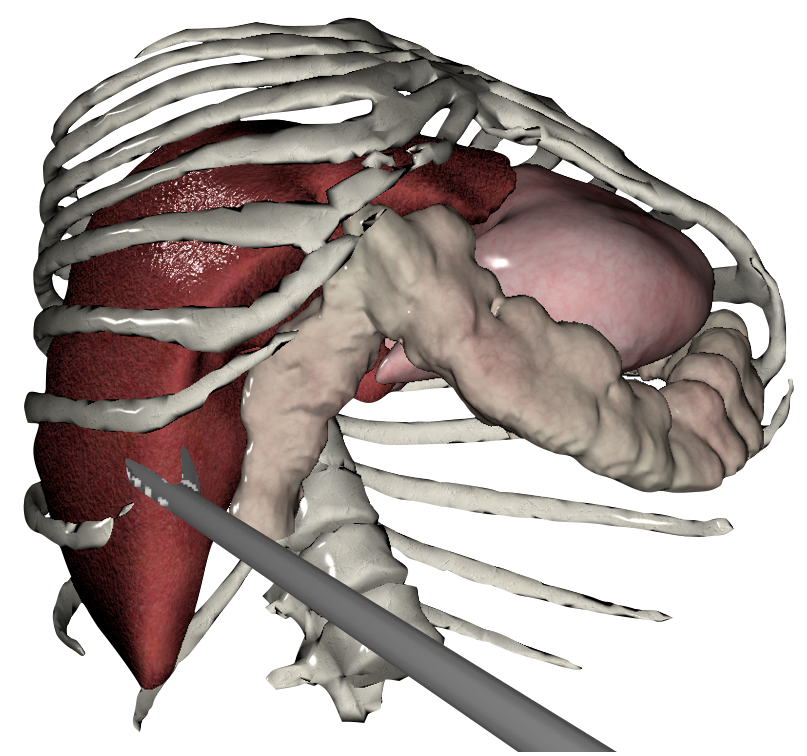
\includegraphics[width=0.48\linewidth]{NewLiver.png}
 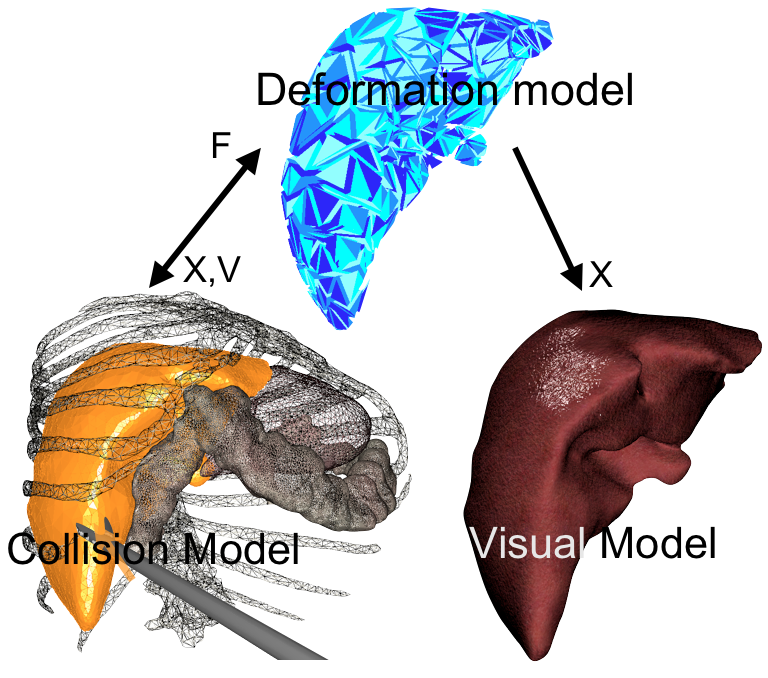
\includegraphics[width=0.5\linewidth]{NewLiverMap.png}
 \caption{A simulated Liver
Left: The simulation of the liver (dataset from IRCAD, France). Right: Three representations are used for the liver: one for the internal mechanics, one for the collisions, and one for the visualization.  These representations are linked using mappings (black arrows).}
 \label{fig:liver-multimodel}
\end{figure}

\section{Solid Mechanics} \label{sec:rigidAndDeformable}


Different models can be employed to discretize a deformable solid continuum as a dynamic or quasi-static system of particles (also called simulation nodes).
The node coordinates are the independent degrees of freedom (DOFs) of the object, and they are typically governed by equations of the following type:
% Some boundary conditions, composed of imposed motion at the node can be applied to the system.
\begin{equation}
 \label{eq:expliciteulerexample}
 \Va = \P \M^{-1} \sum_i \Vf_i (\Vx,\Vv)
\end{equation}
where \Vx and \Vv are the position and velocity vectors, the $\Vf_i$ are the different force functions (volume, surface and external forces in this example), \M is the mass matrix and \P is a projection matrix to  enforce boundary conditions on displacements. Note that the modeling of rigid body dynamics leads to the same type of equations.

The corresponding model in \sofa{} is a set of components connected to a common graph node, as shown in the right of Figure~\ref{fig:liver-mechanical}. 
%
\begin{figure}
 \centering
 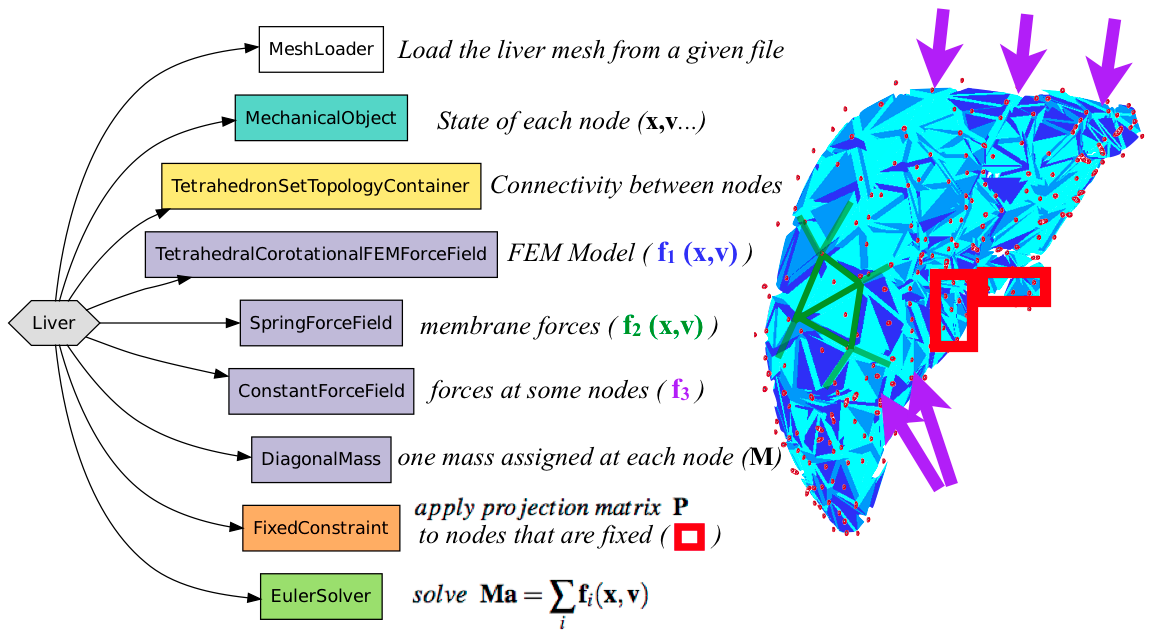
\includegraphics[width=0.95\linewidth]{liver-mechanical2.png}   % generated from ps using: dvipdf -dEPSCrop
 \caption{Mechanical model of a liver. In order to facilitate the combination of models and algorithms, the liver is described as a composition of specialized components.}
 \label{fig:liver-mechanical}
\end{figure}
%
Each component is responsible for a small number of tasks implemented using virtual functions in an object-oriented approach.
Each operator in Equation~\ref{eq:expliciteulerexample} corresponds to a component.
\textit{MeshLoader} is used to read the topology and the geometry.
The coordinate vector \Vx of the mesh nodes and all the other state vectors (velocity \Vv, net force $\sum \Vf$, etc.) are stored in \textit{MechanicalObject}, which is the core component of the mechanical model.
A tetrahedral connectivity is stored in \textit{TetrahedronSetTopologyContainer}, and made available to other components such as \textit{TetrahedralCorotationalFEMForceField}, which accumulates one of the terms of the force sum using the Finite Element method.
The two other terms come from \textit{SpringForceField}, which accumulates the forces generated by the membrane, and  \textit{ConstantForceField}, which accumulates external forces to a given subset of simulation nodes (for instance the pressure exerted by the diaphragm on the liver).
\textit{DiagonalMass} is used to implement the product with matrix $\M^{-1}$.
\textit{FixedConstraint} implements the product with matrix $\P$ to cancel the displacements of the squared particles.
\textit{EulerSolver} implements the logic of time integration.

This approach is highly modular because the components are completely independent of each other and are implemented using C++ classes with a reduced number of abstract functions. 
For instance, in the example of figure \ref{fig:liver-mechanical}, if one want to use a FEM for the membrane force instead of the spring based computation, only \textit{SpringForceField} has to be changed for \textit{TriangleFEMForceField}. Similarly, the mass matrix, stored as diagonal matrix in this example, can be stored as a single scalar value (\textit{UniformMass}) if less accuracy but faster computation is sought, in combination with an iterative solver for instance.



For efficiency, each mechanical state vector contains the values of all the simulation nodes, to avoid multiple call of virtual function resolutions.
The vector size is basically the number of particles times the number of space dimensions. 
We use C++ templates to avoid code redundancy between scalar types (float, double), the types of degrees of freedom (particles, frames, generalized coordinates), and the number of space dimensions.
All the particles in a vector have the same type known at compile time.
Degrees of freedom of different types must be grouped in different objects, possibly connected with interaction forces, as discussed in Section~\ref{sec:interactionforcefield}.
This greatly simplifies the design and allows aggressive compiler optimizations.

More than 30 classes of forces are implemented in SOFA, including springs, FEM for volumetric (tetrahedron or hexahedron) or surface (triangular shell and membrane) deformable objects using corotational or hyperelastic formulations, and for wire or tubular object (beam models meshed with segments), have been implemented.
Different types of springs allow for easy and fast modeling of the deformations (bending, compression/traction, volume, interactions between two bodies, joints...).
In rigid objects, the main components are the degrees of freedom (a single frame with 3 rotations and 3 translations) and the mass matrix that contains the inertia of the object. 
Surfaces can be attached to objects using \textit{mappings}, as discussed in Section~\ref{sec:mappings}.


\section{Collision models} \label{sec:collisionModels}
When a lot of primitives comes into contact, collision detection and response can become the bottleneck of a simulation. 
Several collision detection approaches have been implemented: distances between pairs of geometric primitives (triangles and spheres), points in distance fields, distances between colliding meshes using ray-tracing~\cite{HerFauRaf08}, and intersection volume using images~\cite{AFCFDK10}
The collision pipeline is described in section \ref{sec:collision} with more details. 

In order to adapt the models to the data structure of the different collision algorithms, we have defined a \textit{collision model}.
This model is similar to a mechanical model, except that its topology and its geometry are of its own and can be  stored in a data structure dedicated to collision detection. 
For instance, the component \textit{TriangleModel} is the interface for the computation of collision detection on a triangular mesh surfaces.

If the collision of a given simulation takes too much time, or to reduce the number of collision points, the meshes used for collision detection can be chosen less detailed than the mechanical ones. 
In the opposite, if precise collision detection and response is needed with  smooth surfaces, it is sometimes suitable to use more detailed mesh for collision detection.











%%%%%%%%%%%%%%%%%%%%%%%%%%%%%%%
\section{Visual models} \label{sec:visual}

In the context of surgical simulation for training, to reach the state of what is often called \textit{suspension of disbelief} i.e. when the user forgets that he or she is dealing with a simulator, there are other factors than the mechanical behavior. 
Realistic rendering is one of them. 
It involves visually recreating the operating field with as much detail as possible, as well as reproducing visual effects such as bleeding, smoke, lens deformation, etc.
The main feature of the visual model of SOFA is that the meshes used for the visualization can be disconnected from the models used for the simulation. 
The mappings described in section \ref{sec:mappings} maintain the coherency between them.
Hence, SOFA simulation results can easily be displayed using models much more detailed than used for internal mechanics, and rendered using external libraries such as OGRE\footnote{www.ogre3d.org} and Open Scene Graph\footnote{www.openscenegraph.org}.

We have also implemented our own rendering library based on openGL. 
This library allows for modeling and render the visual effects that occurs during an intervention or the images that the surgeon is watching during the procedure.
For instance, in the context of interventional radiology simulator, we have developed  a dedicated interactive rendering of X-ray and fluoroscopic images. 





 \section{Mappings} \label{sec:mappings}
As previously discussed, objects simulated in \sofa, like the liver in Figure \ref{fig:liver-multimodel}, typically rely on several models: one for the internal model, one for collision, and one for the visual rendering. 
To enforce consistency, one of them, typically the internal model, acting as the master, imposes its displacements to slaves (typically the visual model and the collision model), using \textit{mappings}.
Mapped model can be masters of other models in turn, creating a hierarchy whith the independent DOFs at the root.
Figure \ref{fig:hierarchy} illustrates the hierarchies of two objects. The visual models, in additional branches, are omitted for clarity. When contact models collide, additional geometry is necessary to model the contacting points.
This additional geometry is represented in an additional level connected to the models, as depicted in the figure. 


The positions $\vec x_c$ of a child model are computed by the mapping based on the positions $\vec x_p$ of the master using a function $\JNL$. 
\begin{equation} %\label{eq:mapV}
\vec x_c =\JNL(\vec x_p)
\end{equation}
% In the particular case of a FEM model, this mapping function can rely on the underlying interpolation of the model. 
% 
% 
% These mapping are implemented in a very generic way and allows the control of any kind of slave model $\vec x_1 = \JNL_1(\vec x_0)$ given the position of a master model $\vec x_0$ . 
The velocities can be mapped in a similar way:
\begin{equation}
\vec v_c = \mat J \vec v_p
\end{equation}
The Jacobian matrix $\mat J = \frac{\partial \vec x_c}{\partial \vec x_p}$ encodes the linear relation between the parent and child velocities.
It also holds on accelerations, with an additional offset due to velocities when the position mapping $\JNL$ is nonlinear.
In linear mappings, operators $\JNL$ and $\J$ are the same, otherwise $\JNL$ is nonlinear with respect to $x_p$ and it can not be written as a matrix.
For surfaces embedded in deformable cells, matrix $\J$~contains the barycentric coordinates (it corresponds to linear interpolation in FEM).
For surfaces attached to rigid bodies, each row of the matrix encodes the usual relation $v = \dot o + \omega \times (x-o)$ for each vertex. 

The positions and the velocities are propagated top-down in the hierarchy. 
Conversely, the forces are propagated bottom-up, up to the independent DOFs, where Newton's law $\vec f=\M\vec a$ is applied. 
Given forces $\vec f_c$ applied to a child model, the mapping computes and accumulates the equivalent forces $\vec f_p$ applied to its parent. 
Since equivalent forces must have the same power, the following relation holds:
$$
\vec v_{p}^T \vec f_p = \vec v_c^T \vec f_c
$$
The kinematic relation $\vec v_{c} = \J \vec v_{p}$ allows us to rewrite the previous equation as
$$
\vec v_{p}^T \vec f_{p} = \vec v_{p}^T \J^T \vec f_c
$$
Since this relation holds for all velocities $\vec v_p$, the principle of virtual work allows us to simplify the previous equation to obtain:
\begin{equation} \label{eq:mapF}
\vec f_{p} = \J^T \vec f_c
\end{equation}
When a model has several children, each child accumulates its contribution to the parent forces using its mapping. 
This hierarchical kinematic model allows us to compute displacements and to apply forces at all levels.
%
\begin{figure}
 \centering
 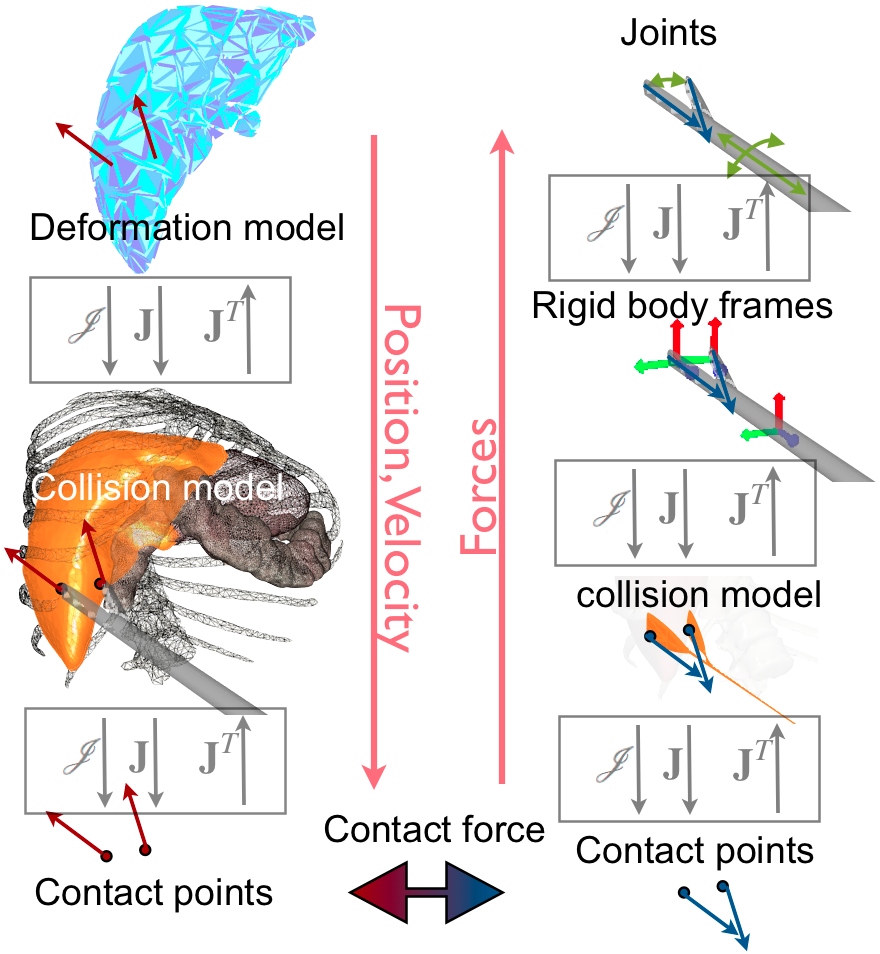
\includegraphics[width=0.9\linewidth]{MappingScheme.png}
 \caption{Mappings from the DOFs to the contact point. Right (top to bottom): The Mechanical model of the liver is based on Finite Element model. A triangular mesh is mapped for collision detection with the surface. The two contact points found by the collision detection (with the grasper) are mapped on the collision model. 
 Left (bottom to top): the contact points are also mapped on the collision model of the grasper. This collision model is a simplification of the grasper shape and is mapped on the rigid body frames. The motion of these frame is mapped on the state of the joints which are the independent DOFs of the grasper.
}
 \label{fig:hierarchy}
\end{figure}
%
So far, $22$ variants of mappings have been implemented to attach models to rigid objects and deformable primitives such as tetrahedra, hexahedral grids, splines, blended frames, flexible beams and scalar fields.
Mappings are also be used to connect generalized coordinates, such as joint angles, to world-space geometry, as in the grasper of Figure~\ref{fig:hierarchy}.


%% attacher de la g�om�trie
%
%
%They are not independent variables, since the positions and velocities are bound to the independent DOF.
%We say that a child geometrical model $1$ is \textit{mapped} from its parent model $0$,
% using a kinematic operator which we call \textit{mapping}. It implements the kinematic relations:
%\begin{eqnarray*} %\label{eq:mapV}
%\vec x_1 &=&\JNL_1(\vec x_0)\\ 
%\vec v_1 &=& \mat J_1 \vec v_0
%\end{eqnarray*}
%Mappings allow to attach polygonal shapes (like the tool shape in Figure~\ref{fig:hierarchy}, with point DOFs) to rigid bodies (with frame DOFs) using local coordinates, or to embed the shapes in deformable cells using barycentric coordinates (like the deformable liver in Figure~\ref{fig:hierarchy}), among other possibilities.
%Matrix $\mat J_1 = \frac{\partial \vec x_1}{\partial \vec x_0}$ encodes the linear relation between the parent and child velocities.
%It also holds on accelerations, with an additional offset due to velocities when the position mapping \JNL is nonlinear.
%In linear mappings, operators \JNL and \J are the same, otherwise \JNL is nonlinear with respect to $x_0$ and it can not be written as a matrix.
%For surfaces embedded in deformable cells, matrix \J~contains the barycentric coordinates. 
%For surfaces attached to rigid bodies, each row of the matrix encodes the usual relation $v = \dot o + \omega \times (x-o)$ for each vertex. 
%% Similarly, skins around articulated bodies involve, at each vertex, the weighted  contributions of the rigid bodies. 


%% g�om�trie suppl�mentaire d�e aux contacts
%When shapes collide, additional geometry is necessary to model the contact.
%For instance, when an edge intersects or closely approaches another one, a contact force is typically applied to the intersection point or to the pair of points.
%The points are defined using their barycentric coordinates with respect to the edge vertices. 
%% Other relations can be used, depending on the kind of geometrical primitives in contact.
%This additional geometry can be represented in another geometrical layer connected to the shape by a mapping, as illustrated in the bottom of Figure~\ref{fig:hierarchy}.
%% This layer is also connected to the shape using mappings:
%% \begin{eqnarray*} %\label{eq:mapV}
%% x_2 &=&\JNL_2(x_1)\\ 
%% v_2 &=&J_2 v_1 
%% \end{eqnarray*}
%
%We generalize this approach to tree-like hierarchies of geometries, with the independent DOFs at the root. 
%For instance, the independent DOFs may have two children, one for collision using a coarse mesh, and the other for rendering using a finer mesh.
%The hierarchy have more levels, for instance, to attach collision spheres to a mesh embedded in a deformable grid. 
%The synchronization between these models is automatically guaranteed by their attachment to their common ancestor, using graph visitors as explained in Section~\ref{sec:visitors}.
%Positions and velocities are propagated top-down in the hierarchy. Conversely, the forces are propagated bottom-up, up to the independent DOFs, where Newton's law $f=ma$ is applied. 
%Given forces $f_c$ applied to a child model, the mapping computes and accumulates the equivalent forces $\vec f_p$ applied to its parent. 
%Since equivalent forces must have the same power, the following relation holds:


% In implicit simulation methods, one needs to consider force changes $\vec{df}$ corresponding to small displacements $\vec{dx}$ of the independent DOF.
% This involves the forces applied to the independent DOF, but also the forces are applied to mapped DOFs.
% Let $0$ denote the independent DOF.%, and $n$ a level mapped through $n$ mappings indexed from $0,1$ to $n-1,n$.
% At each hierarchy node $i$, let $\mat K_{ii}$ be the stiffness matrix corresponding to the forces applied to the local DOF.
% The local displacement is :
% \begin{equation} \label{eq:displacementsTopDown}
%  \vec{dx}_{i} = \prod_{j=1}^{i}\mat J_{j,j-1} \vec{dx}_{0}
% \end{equation}
% where $\prod_{j=1}^{i}\mat J_{j,j-1} = \mat J_{i,i-1}...\mat J_{1,0}$ is the product of the matrices of the mappings in the path from the independent DOF to node $i$.
% The matrix-vector product can be efficiently computed during one top-down traversal of the hierarchy, with one matrix-vector product at each level, without any matrix-matrix product.
% Conversely, the resulting force change on the independent DOFs is:
% \begin{equation} \label{eq:forcesBottomUp}
%  \vec{df}_{0} = \left( \prod_{j=1}^{i}\mat J_{j,j-1} \right)^T \vec{df}_{i}
% \end{equation}
% where $\left( \prod_{j=1}^{i}\mat J_{j,j-1} \right)^T = \mat J_{1,0}^T...\mat J_{i,i-1}^T$ is the product of the transposed matrices of the mappings in the path from node $i$ to the independent DOF.
% This matrix-vector product can be efficiently computed using matrix-vector products during one bottom-up traversal of the hierarchy.

%Figure~\ref{fig:liver-mechanical-spheres} shows a sphere-based collision model attached to the mechanical model of Figure~\ref{fig:liver-mechanical}. 
%The position vector of the collision model is the set of 3d coordinates of the sphere centers, defined by their barycentric coordinates stored in the BarycentricMapping.
%\begin{figure}
% \centering
% 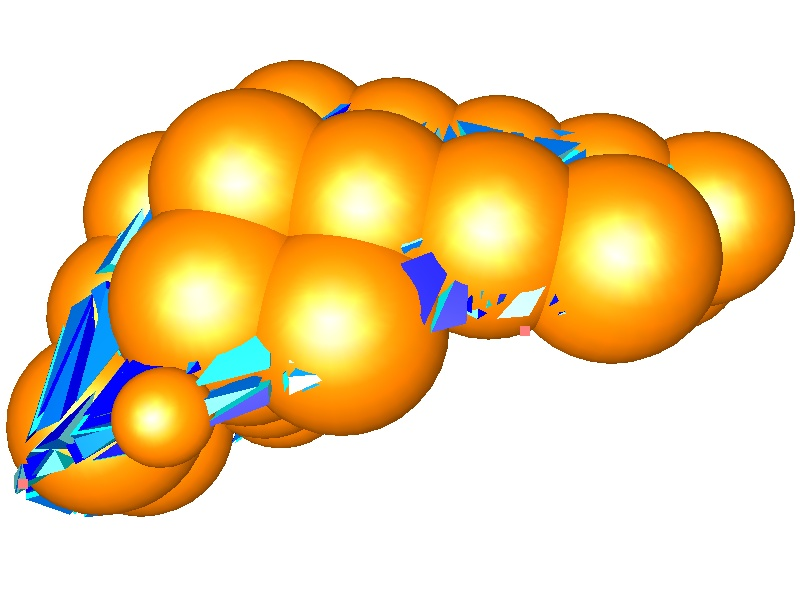
\includegraphics[width=0.4\linewidth]{liver-spheres-superimposed.jpg}
% 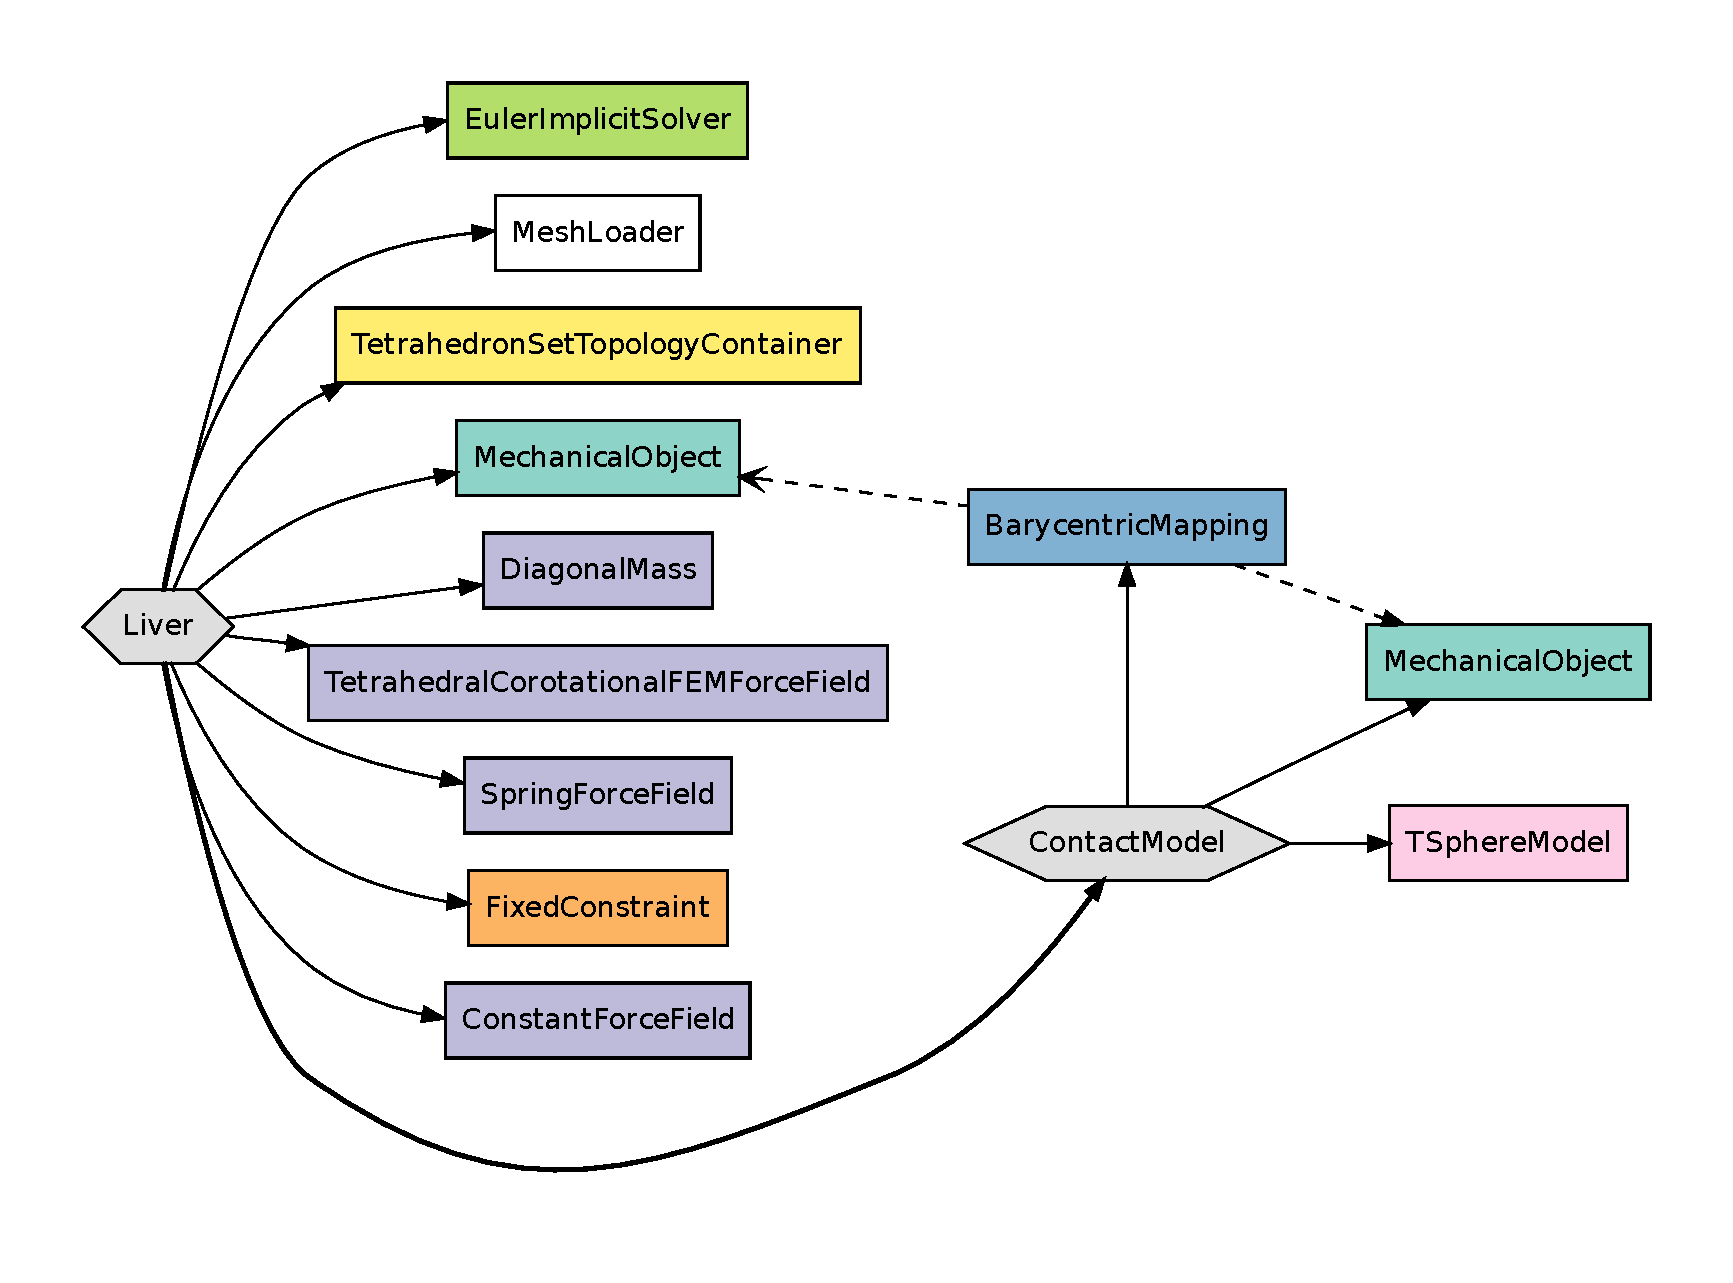
\includegraphics[width=0.56\linewidth]{liver-spheres.pdf}   % generated from ps using: dvipdf -dEPSCrop
% \caption{Left: mechanical (in blue) and collision (in yellow) models of a liver. Right: the corresponding scene graph. The plain arrows denote hierarchy, while the stippled arrows represent connections.}
% \label{fig:liver-mechanical-spheres}
%\end{figure}







\chapter{Data Structure}
The organization of simulation data is a complex issue. We have identified three relevant levels, and proposed different solutions for each of them.
The coarsest structure is the scenegraph, used to hierarchically organize the groups of objects and their multi-models.
At a finer scale, the attributes of the components can be linked by relations.
Finally, the geometrical models and the topological changes deserve a special attention.
\graphicspath{{../datastructure/}}  % to include images
\section{Scene-Graph}
% \subsection{Multiple objects}\label{sec:multiple}
When the simulation involves several objects, we model them as different branches in a scenegraph data structure.
In the example shown in Figure~\ref{fig:twoObjects}, the scene contains two objects animated using different time integrators, collision detection components (discussed in Section~\ref{sec:collision}), an interaction force, and a camera to display the objects.
The root node does not contain DOFs.
It is used to contain the components which are common to its child nodes.
\begin{figure}
 \begin{center}
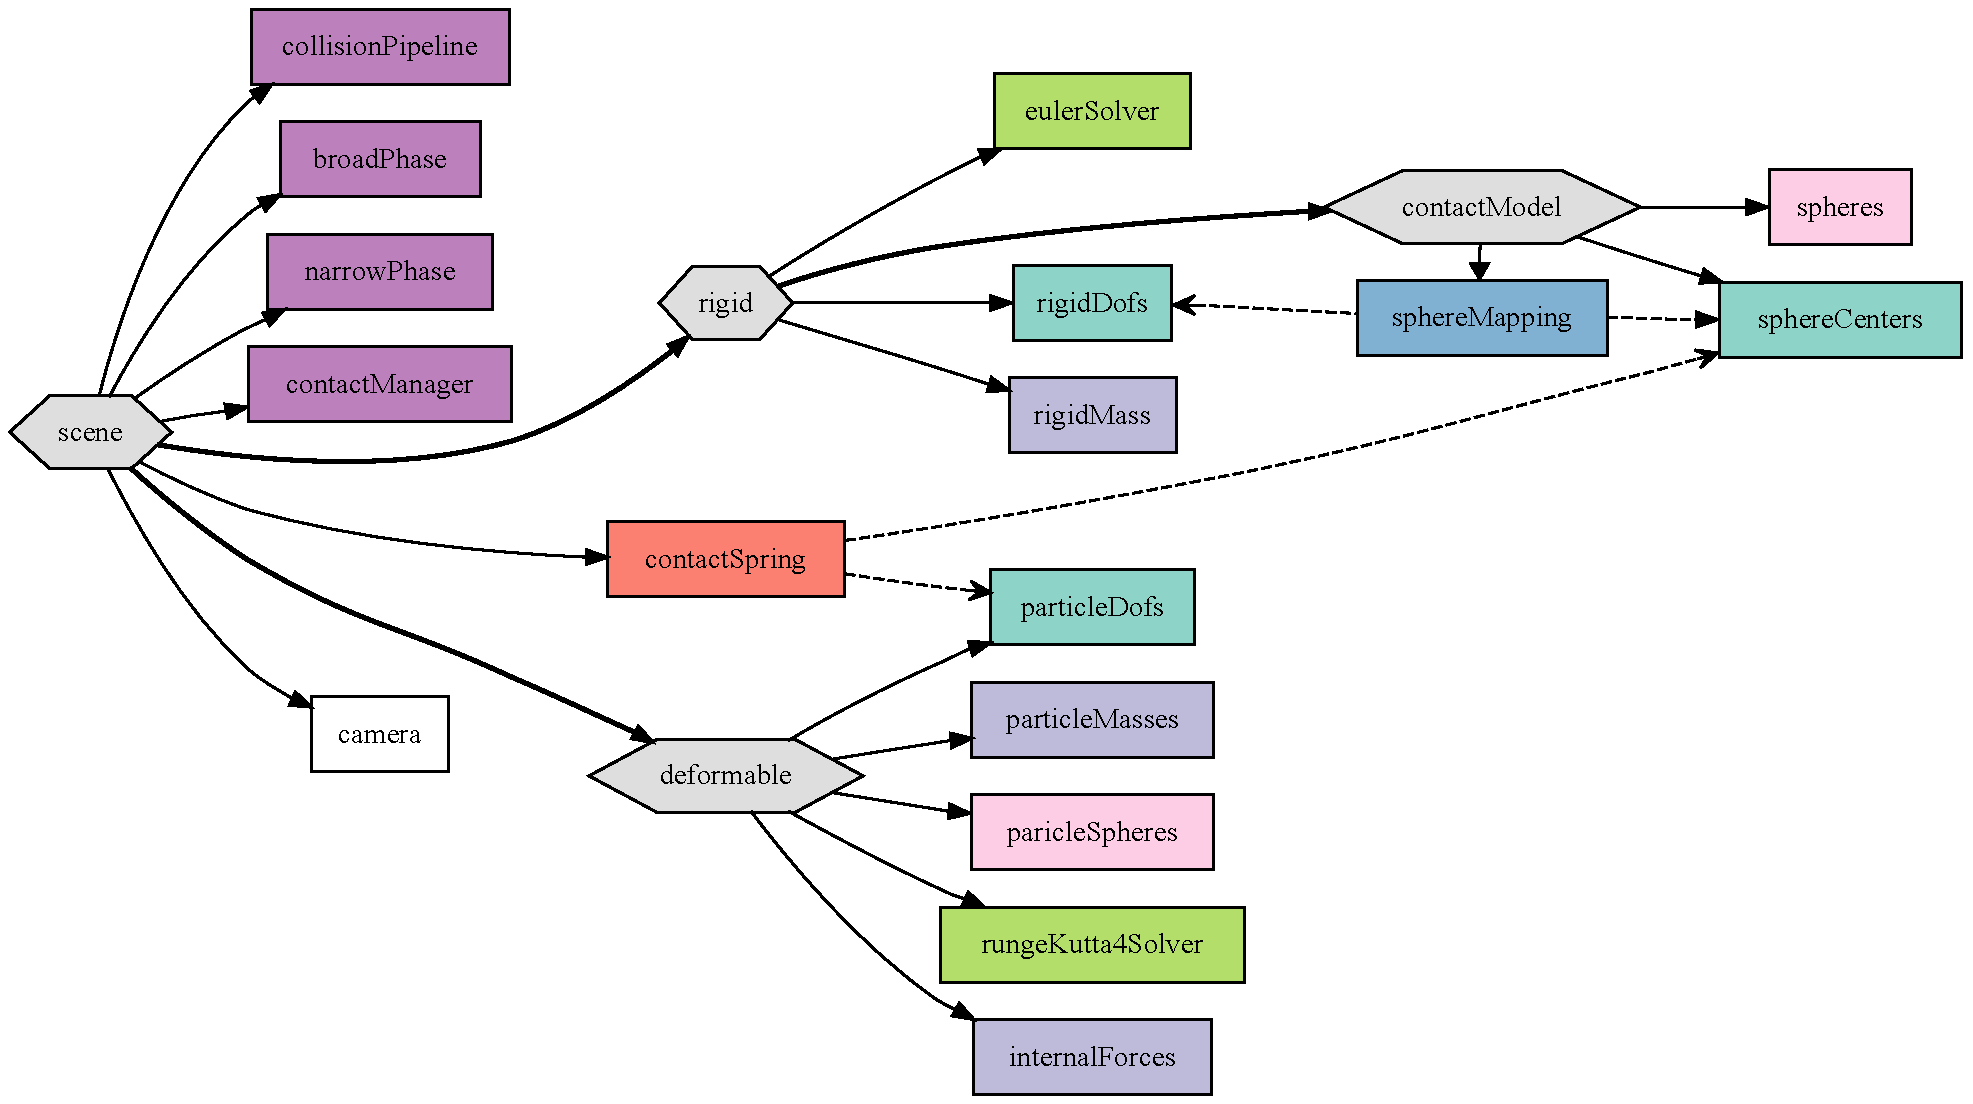
\includegraphics[width=0.98\linewidth]{twoObjects.pdf}
 \caption{A scenegraph with collision detection and two independent objects interacting through a spring.}                                                                      
 \label{fig:twoObjects}
\end{center}
\end{figure}
% Applying the same ODE solver to all the objects is as simple as attaching the corresponding component to the common ancestor node.
% This allows to process the objects and their interaction forces in a common equation system, which is necessary when stiff interaction forces or Lagrange multipliers are used for coupling the objects. 
% When each object has its own solver, the interaction force is considered constant during the time step.

Scenegraphs are popular in Computer Graphics due to their versatility.
The data structure is processed using visitors (discussed in Section~\ref{sec:visitors}) which apply virtual functions to each node they traverse, which in turn apply virtual functions to the components they contain.
% , and the visitor-based approach presented in Section~\ref{sec:visitors} allows us to apply operations to all the branches, possibly in parallel. 
In basic scenegraph frameworks, the visitors are exclusively fired from an external control structure such as the main loop of the application.
In \sofa, the components are allowed to suspend the current traversal to send an arbitrary number of other visitors, then to resume or to prune the suspended visitor.
This allows us to implement global algorithms (typically ODE solution or collision detection), such as the explicit Euler velocity update of Equation~\ref{eq:expliciteulerexample}, in components.
This neatly decouples the physical model from the simulation algorithms, in sharp contrast with dataflow graphs which intricate data and operators in the same graph.
Replacing a time integrator requires the replacement of one component in our scenegraph, whereas the corresponding dataflow graph would have to be completely rewritten.




Interactions between objects may be handled using penalty forces or Lagrange multipliers. 
In all cases, a component connected to the two objects is necessary to geometrically model the contact and compute the interaction forces.
This component being shared between the two objects, it is located in their common ancestor node.
The coupling created by penalty forces should be seen as soft or stiff, depending on the stiffness and the size of time step~\cite{baraff98large}.
A soft coupling can be modeled by an interaction force constant during each time step.
In this case, each object can be animated using its own, possibly different, ODE solver.
% The interaction force is computed and accumulated  when the AnimateVisitor traverses the ancestor nodes before reaching each solver in their child branches.
% This ensures that the object undergo opposite interaction forces during the time step, but it requires the synchronization of the object at the end of each time step.
% Animating the two objects at different time steps would be possible, using each solver independently instead of a common AnimateVisitor, but this would require an additional mechanism to update the interaction and enforce Newton's third law on opposite forces.
The assumption of constant interaction force during each time step is compatible with all explicit time integration methods.
However, when the interaction forces are stiff, implicit integration is necessary to apply large time steps without instabilities.
This requires the solution of an equation system involving the two objects as well as their interaction force together.
In this case, the ODE solver is placed in the common ancestor node, at the same level as the interaction component.
This is also true for constraint-based interaction which requires the computation of Lagrange multipliers based on interaction Jacobians. 
% \todo{illustrer sur une figure}
% We call it \textit{hard coupling} when the interacting objects and the interaction forces need to be solved simultaneously in a common equation system.
% This includes stiff penalty forces and Lagrange multipliers.
Due to the superlinear time complexity of equation solvers, it is generally more efficient to process independent interaction groups using separated solvers rather than a unique solver.

% 
% Contact interactions created during the simulation may be soft, stiff of constraint-based, depending on the collision response stategy, as explained in Section~\ref{sec:collision}.
% In case of hard coupling, a group manager is used to gather objects in the smallest possible groups.


% \subsubsection{The context} \label{sec:components}
% \SC{I would remove this subsection - it is redundant with some of the other text}
% 
% % \todo{Description plus détaillée des composants : principe de séparation des données (State,TopoContainer), des calculs (FF,TopoModifier,...), et des dépendances (Node)}
% % 
% % \todo{Présentation de l'utilisation des templates : comment ils permettent dans les composants d'avoir des codes génériques tout en étant instancié et optimisé par le compilateurs pour chaque type de DOF.}
% All the components acting on the same DOFs are gathered in a common node, which main contain: 
% % A node may represent a set of physical objects, such as the root of the scene or a collision group, using the list of child nodes.
% % Groups may contain algorithm components, applied to all the children using graph visitors as explained in Section~\ref{sec:visitors}. 
% % These include ODE solvers to integrate time, collision detection algorithms, and MasterSolvers to schedule the formers.
% % Groups may also include components associated with interactions between the child nodes, as discussed in Section~\ref{sec:interactions}.
% % A node may also represent one kinematic layer of a physical object, i.e. a set of components associated with the same degrees of freedom.
% % This includes: 
% \begin{itemize}
%  \item a container of state vectors, to represent coordinates, velocities, forces, accelerations and any auxiliary vector used by the algorithms. Each state vector contains the values associated to all the nodes. All the following components in this list read and write the state vectors in this component.
%  \item a list of topology containers, to model mesh edges, faces and cells based on node indices.
%  \item a mass, to compute accelerations based on forces, and momentums based on velocities.
%  \item a list of force functions, to accumulate forces based on positions and velocities. They can be used to model internal or external forces, including force boundary conditions.
%  \item a list of projective constraints, to filter the state vectors to cancel forbidden displacements. They can be used to apply displacement boundary conditions to each indendent DOF.
%  \item lists of geometrical primitives used in collision detection.
%  \item a list of child nodes, to create hierarchies and complex scenes (see sections~\ref{sec:mappings} and \ref{sec:scenes})
%  \item a mapping, to synchronize the local DOFs with master DOFs higher in the hierarchy
%  \item a list of constraints to handle using Lagrange multipliers, more complex but more general than projective constraints. They can be used to apply constraints to non-independent DOFs.
%  \item lists of components implementing algorithms for collision detection(\ref{sec:collision}) and the solution of equations (section~\ref{sec:odesolvers})
% \end{itemize}
% While most of the data is private, some is available to all the components, especially the topology and the state vectors. 
% % These attributes are used by the visitors to access the components during the graph traversals.
% % The connections between the components attached to the same node are generally implicit, because there is a unique container of state vector and a unique topology, which allows the components to find the necessary data.
% For instance, 
% % a TetrahedronFEMForceField computes viscoelastic forces based on the deformation of tetrahedra. 
% the list of tetrahedra used by a TetrahedralFEMForceField is stored in the local topology container, while the initial and current particle states are stored in the MechanicalObject. 
% The same list of tetrahedra may be used to define the embedding of auxiliary DOFs in children nodes, as discussed in Section~\ref{sec:mappings}.
% % Additionally, nodes contain lists of control components to implement simulation algorithms, such as EulerSolver, as discussed in Section~\ref{sec:control}.



\subsection*{Visitors} \label{sec:visitors}
% The top-down and bottom-up force computation presented in Section~\ref{sec:mappings} is easily generalized to an arbitrarily branched hierarchy with forces applied at all levels.
We implement the simulation using visitors which traverse the scene top-down and bottom-up, and call the corresponding virtual functions at each graph node traversal. 
A possible implementation of the traversal of a tree-like graph is shown in the left of Figure~\ref{fig:visitorTraversal}.
Algorithmic operations on the simulated objects are implemented by deriving the Visitor class and overloading its virtual functions \textit{topDown(~)} and \textit{bottomUp(~)}. 
This approach hides the scene structure (parent, children) from the components, for more implementation flexibility and a better control of the execution model.
The data structure can easily be generalized from strict hierarchies to directed acyclic graphs for more general kinematic dependencies.
Moreover, various parallelism strategies can be applied independently of the mechanical computations performed at each node.
\begin{figure}
\begin{center}
\begin{tabular}{l|r}
\begin{minipage}{0.4\linewidth}
\begin{algorithmic}
\STATE void  \textbf{Visitor::traverse(Node n)}
\STATE bool continue = this.topDown( n )
\IF{continue} 
\FORALL {c child of n} 
\STATE traverse( c ) 
\ENDFOR
\STATE     this.bottomUp( n )
\ENDIF
\end{algorithmic} 
\end{minipage}
 &
\begin{minipage}{0.5\linewidth}
\begin{algorithmic}
% \renewcommand{\algorithmicendfor}{}
% \renewcommand{\algorithmicendif}{}
\STATE bool  \textbf{AnimateVisitor::topDown(Node n)}
\IF{masterSolver} 
\STATE masterSolver.animate(this.dt)
\RETURN false
\ENDIF
\IF{collisionPipeline} 
\STATE collisionPipeline.modelContacts()
\ENDIF
\IF{odeSolver} 
\STATE odeSolver.solve(this.dt)
\RETURN false
\ENDIF
\FORALL {InteractionForce f}
\STATE f.apply()
\ENDFOR
\RETURN true
\end{algorithmic} 
\end{minipage}
\end{tabular}
\end{center}
\caption{Left: a recursive implementation of the visitor traversal. Right: the AnimateVisitor. }
\label{fig:visitorTraversal}
\end{figure}

Forward time stepping is implemented using the \textit{AnimateVisitor} traversal method, shown in the right of Figure~\ref{fig:visitorTraversal}.
Applied to the simple scene in Figure~\ref{fig:liver-mechanical-spheres}, it triggers the ODE solver, which in turn applies its algorithm using visitors for mechanical operations such as propagating states through the mappings or accumulating forces.
Note that the traversal of the AnimateVisitor is pruned when a ODE solver is encountered.
This allows the ODE solver to take control of its subgraph and to overload lower-level solvers, which are not reached by the AnimateVisitor.
In the more complex scene shown in Figure~\ref{fig:twoObjects}, the solver triggers the collision detection, which may create a contact between the chidren, such as contactSpring.
The visitor then triggers the computation of the interaction force, which will be seen by the objects as a constant, external force during the time step.
The visitor then continues the traversal and triggers each object ODE solver.
The default behavior is to model the contacts prior to applying time integration.
To implement other strategies, a \textit{MasterSolve}r can be used to prune the visitor and apply time integration and collision detection in a different order, possibly looping until all collisions are solved.

\begin{figure}
 \centering
 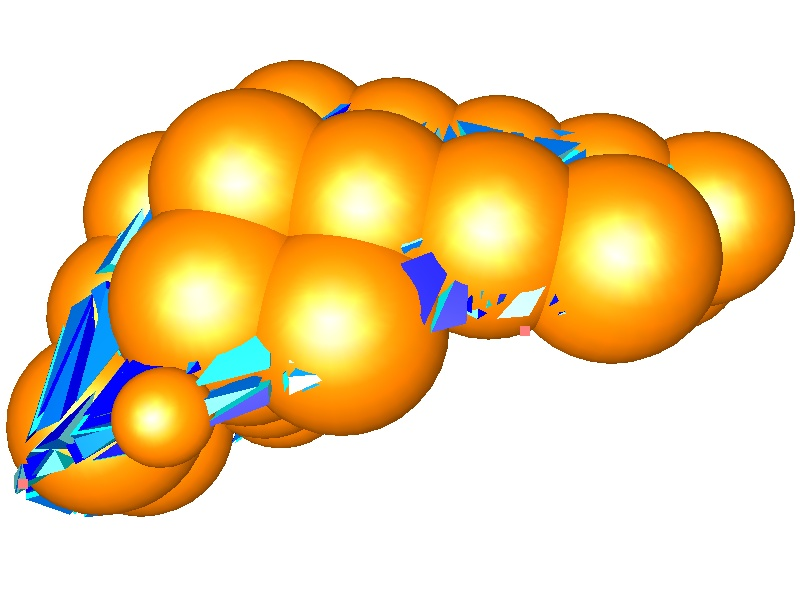
\includegraphics[width=0.4\linewidth]{liver-spheres-superimposed.jpg}
 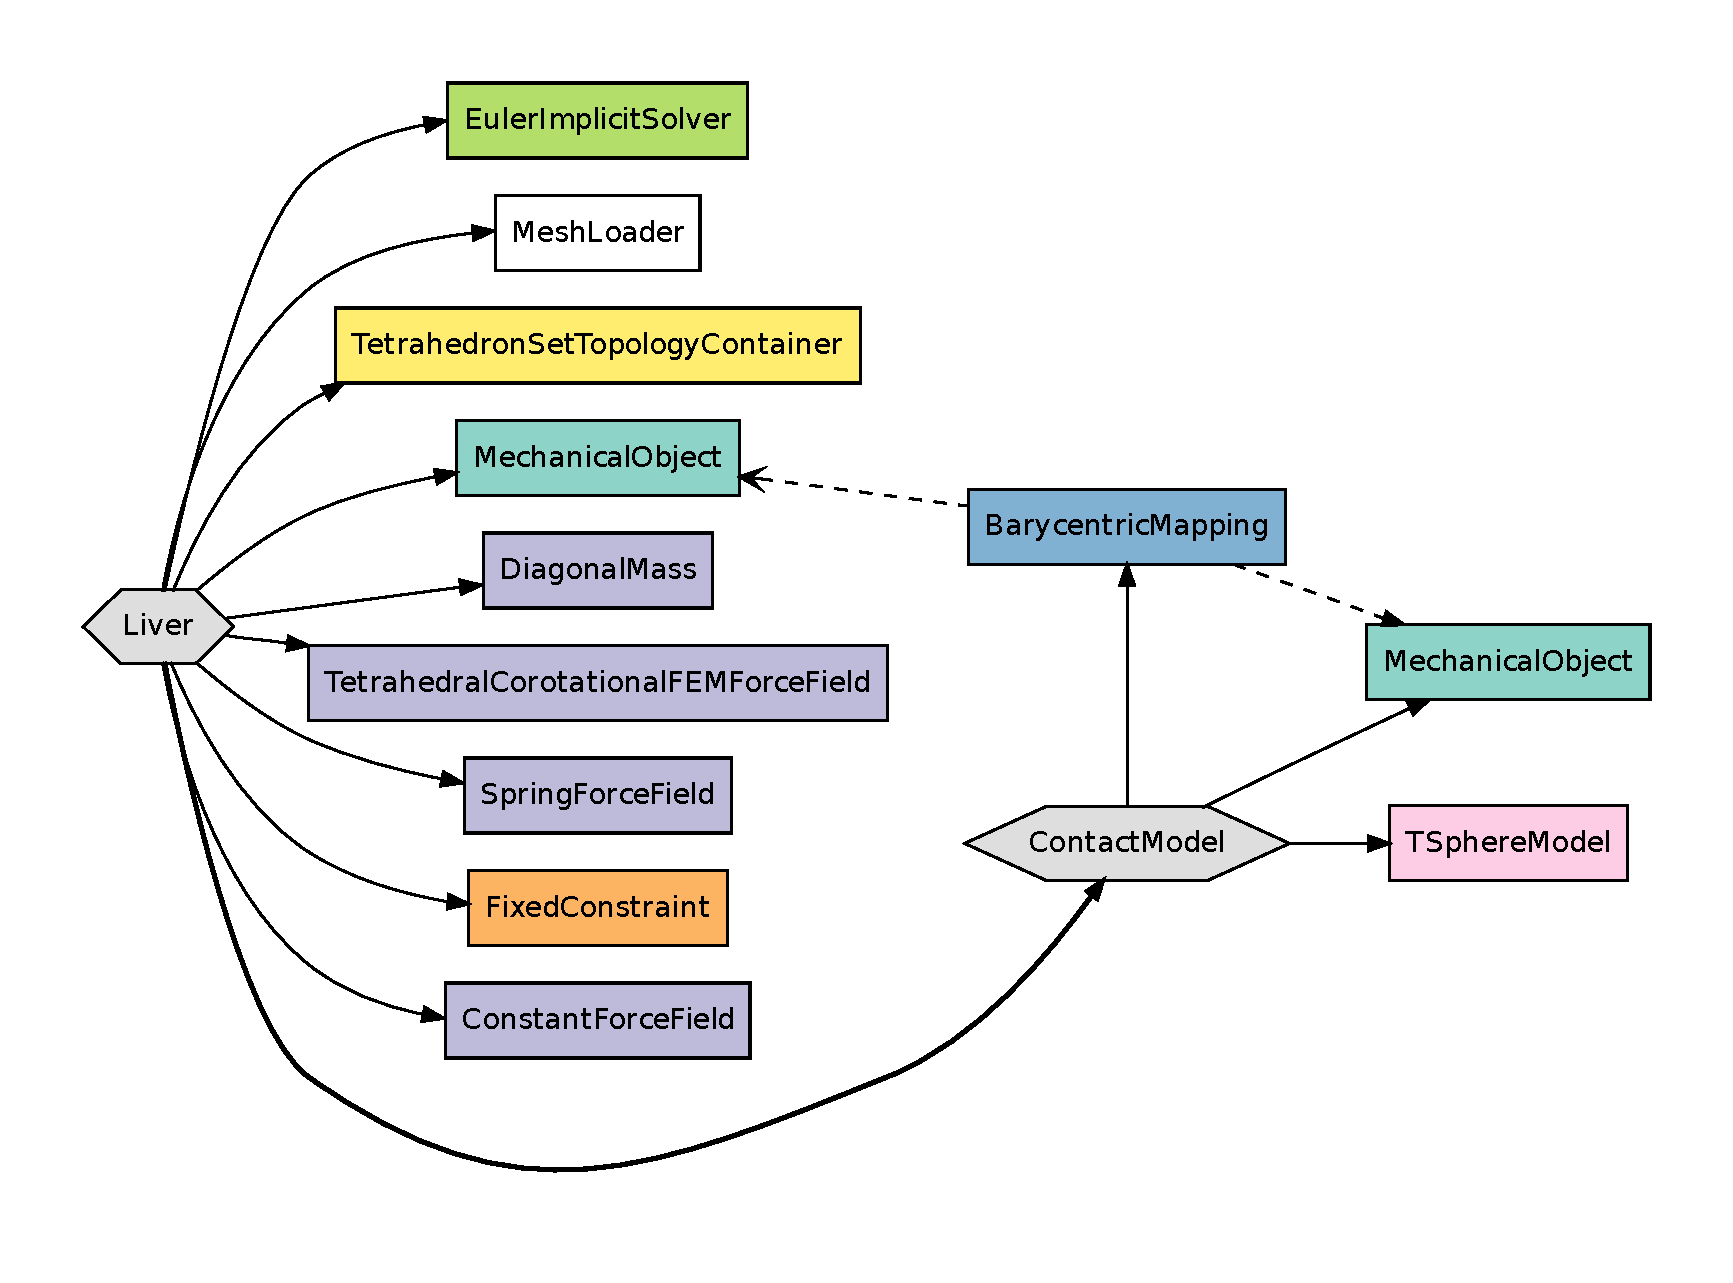
\includegraphics[width=0.56\linewidth]{liver-spheres.pdf}   % generated from ps using: dvipdf -dEPSCrop
 \caption{Left: simple mechanical (in blue) and collision (in yellow) models of a liver. Right: the corresponding scene graph. The plain arrows denote hierarchy, while the stippled arrows represent connections.}
 \label{fig:liver-mechanical-spheres}
\end{figure}


\section{Data, Engines and Tags}

Component parameters are stored in member objects using \textit{Data} containers, templated on the type of attribute they represent.
For instance, the list of particle indices constrained by a FixedConstraint is stored in a \lstinline!Data< vector<unsigned> >!.
These containers provides a reflective API, used for serialization in XML files and the automatic creation of input/output widgets in the user interface, as discussed in Section~\ref{sec:interface}.
% When the same data is needed by different components, each component contains a corresponding Data object, and these Data are synchronized using connections.
%This eases thread-safe programming \SC{true ?} and allows the automatic computation and the update of Data dependencies using operator objects called \textit{Engines}.
We can create connection between Data instances to keep their value synchronized. This is used for instance when a \textit{Loader} component loads several attributes from a file (such as topology, positions, stiffnesses, boundary conditions) which are then connected to one or more components using it as input.
In some cases we need to not simply copy an existing value but compute it from one or several Data. This feature is provided by \textit{Engine} components.
%We can also create connections through an \textit{Engine}, which is used when 
Engines contain input and output Data, and their update method computes the output based on the input.
%When a Data value is changed, the connected Data are flagged as \textit{dirty}, and so on recursively through connections and engine input-outputs.
A mechanism of lazy evaluation is used to recursively flag Data values that are not up-to-date, but they are recomputed only when necessary.
For instance, based on a bounding box and a vector of coordinates, a BoxROI engine computes the list of indices of the coordinates inside the box. These indices can then be used as input of a FixedConstraint to define a fixed boundary condition. With this design, the simulation can transparently be setup either from data stored in static files, or generated automatically with engines.

The network of interconnected Data objects defines a data dependency graph, superimposed on the scene graph.
This two-graph framework is used in other graphics software such as OpenInventor and Maya, where engines are used to generate the animation, by periodically updating the state vectors using time as input. 
However, while this approach works well for straightforward computation pipelines, such as keyframe interpolation, it does not easily allow the branching and loops control structures used in sophisticated physical simulation algorithms.
It is also a rather low-level representation, essentially encoding every computation steps required to compute a given Data.
Consequently, we only use Engines to implement straightforward relations between the parameters of the model, which may remain unchanged during the simulation.
% \SC{ True? Could we really not use this mechanism instead of mappings? It  would be nice to explain the difference with the mappings ;-)}
In \sofa{}, the state update algorithms are instead determined by combining several components, communicating through scenegraph visitors, as explained in Section~\ref{sec:solvers}.

\subsection*{Objects and node tagging (\textcode{Tag} and \textcode{TagSet}).}

The goal of the introduction of tags is to provide one of the pieces necessary to support non-mechanical states (electrical potentials, constrast agent concentrations) as well as cleaner non-geometrical mechanical states (fluid dynamics, reduced-coordinate articulations).
For example, in a simulation involving blood in deformable vessels, we would use two tags to distinguish the different states : mechanical, fluid.
These tags will be used to easily work with only a subset of the components, so that the mechanical solver works on positions and forcefields but don't interferes with blood flow and pressure, and inversely for the fluid solver (see \footnote{http://wiki.sofa-framework.org/tdev/wiki/Notes/ProposalGenericStates} ).
We decided on using there tags instead of extending the class hierarchy as was done before with the \textcode{State} and \textcode{MechanicalState} classes.
A hierarchy is fine when we have only one feature that we want to differentiate on (such as base vs mechanical vs electrical), but when we add other criteria (lagrangian geometry vs eulerian vs reduced generalized coordinates, velocity vs vorticity, independent vs mapped DOFs) it is no longer manageable as specialized classes.
A secondary use of these tags is to replace existing subsets mechanisms within CollisionModels (r2441) and Constraints (r3121).
The design is based on the following elements.
Tags are added to BaseObject, as a list of string (internally converted to a list of unique ids for faster processing).
All visitors now filter the objects they process based on their list of tags.
All solvers by default copy their own list of tags to the visitors they execute, so that they only affect the objects with the same tags as they have (TODO: this is currently broken). 

\newpage
\section{How to use mesh topologies in SOFA}

H. Delingette, B. Andr�

\subsection{Introduction}

While mesh geometry describes where mesh vertices are located in space, mesh topology tells 
how vertices are connected to each other by edges, triangles or any type of mesh element. 
Both information are required on a computational mesh to perform :

\begin{itemize}

 \item \textbf{Mesh Visualization},

 \item \textbf{Collision detection} : some collision detection are mesh based (e.g.
triangles or edges),

 \item \textbf{Mechanical Modeling} : deforming a mesh also requires to the
knowledge of a mesh topology. For instance a spring mass model
requires knowing about the edges that connects pair of vertices,

 \item \textbf{Haptic rendering},

 \item \textbf{Description of scalar} (temperature, electric potential, etc.) or
vectorial fields (speed, fiber orientation, etc.)

\end{itemize}

Since topological changes are essential for surgery simulators, a common difficulty when designing those simulators is to ensure that the visual, mechanical, haptic and collision behavior of all meshes stay valid and consistent upon any topological change. 

Our approach to  handle topological changes is modular since each software component (collision detection, mechanical solver$\ldots$) may be written with little knowledge about the nature of other components. It is versatile because any type of topological changes can be handled with the proposed design. 

Our objective to keep a modular design implies that mesh related information (such as mechanical or visual properties) is not centralized in the mesh data structure but is stored in the software components that are using this information. Furthermore, we manage an efficient and direct storage of information into arrays despite the renumbering of elements that occur during topological changes.

\subsection{Family of Topologies} 


We focus the topology description on meshes that are cellular complexes made of $k$-simplices (triangulations, tetrahedralisation) or $k$-cubes (quad or hexahedron meshes). These meshes are the most commonly used in real-time surgery simulation and can be hierarchically decomposed into $k$-cells, edges being $1$-cells, triangles and quads being $2$-cells, tetrahedron and hexahedron being $3$-cells. 
To take advantage of this feature, the  different mesh topologies are structured as a family tree (see Fig.~\ref{fig:BW_Topology_Family_Tree}) where children topologies are made of their parent topology. This hierarchy makes the design of simulation components very versatile since a component working on a given mesh topology type will also work on derived types. For instance a spring-mass mechanical component only requires the knowledge of a list of edges (an {\em Edge Set Topology} as described in Fig.~\ref{fig:BW_Topology_Family_Tree}) to be effective. With the proposed design, this component can be used with no changes on triangulation or hexahedral meshes.
 
The proposed hierarchy makes also a distinction between conformal and manifold meshes. While most common FEM components require a mesh to be conformal (but not necessarily manifold), many high-level software components (such as cutting, contact, haptic feedback algorithms) require the mesh to be a manifold where a surface normal is well-defined at each vertex.   


\begin{figure}[ht]
    \centering
        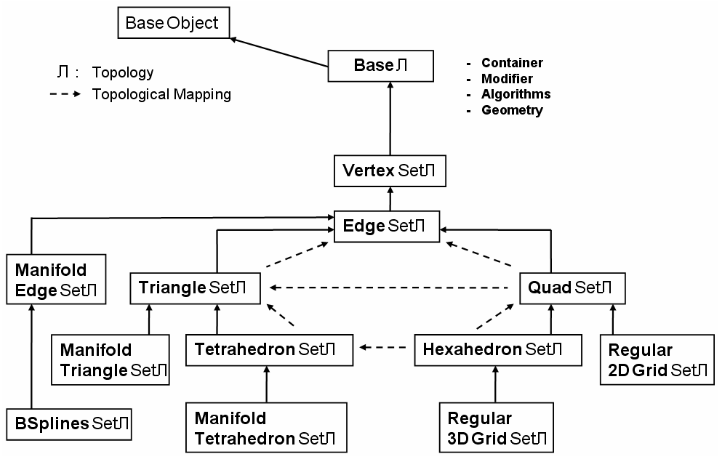
\includegraphics[width=0.85\textwidth]{topology/BW_Topology_Family_Tree.png}
     \caption{Family tree of topology objects. Dashed arrows indicate possible {\em Topological Mappings} from a topology object to another.}
    \label{fig:BW_Topology_Family_Tree}
\end{figure}

Topology objects are composed of four functional members:{\em Container}, {\em Modifier}, {\em Algorithms} and {\em Geometry}.

\begin{itemize}

 \item The {\em Container} member creates and updates when needed two complementary arrays (see Fig.~\ref{fig:BW_Sub_Shell_Diagram}). The former describes the $l$-cells included in a single $k$-cell, $l<k$, while the latter gives the $k$-cells adjacent to a single $l$-cell.
 
 \item The {\em Modifier} member provides low-level methods that implement elementary topological changes such as the removal or addition of an element. 
 
 \item The {\em Algorithms} member provides high-level topological modification methods (cutting, refinement) which decompose complex tasks into low-level ones). 
 
 \item The {\em Geometry} member provides geometrical information about the mesh ({\em e.g.} length, normal, curvature, ...) and requires the knowledge of the vertex positions stored in the {\em Degrees of Freedom} component. 
 
\end{itemize}


\begin{figure}[ht]
    \centering
        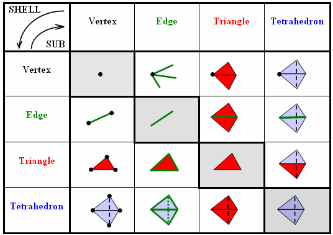
\includegraphics[width=0.6\textwidth]{topology/Sub_Shell_Diagram}
    \caption{The two topological arrays stored in a {\em Container} correspond to the upper and lower triangular entries of this table. The upper entries provide the $k$-cells adjacent to a $l$-cell, $l<k$. The lower entries describe the $l$-cells included in a $k$-cell. Similar table exists for quad and hexahedron elements.}
    \label{fig:BW_Sub_Shell_Diagram}
\end{figure}

\subsection{Component-Related Data Structure}

A key feature of our design is that containers storing mesh information (material stiffness, list of fixed vertices, nodal masses, ...) are stored in {\em components} and spread out in the simulation tree. This modular approach is in sharp contrast with a centralized storage of information in the mesh data structure through the use of generic pointers or template classes.  

Another choice is that most containers are simple arrays with contiguous memory storage and a short direct access time.
This is important for real-time simulation, but bears some drawbacks when elements of these arrays are being removed since it entails the renumbering of elements. For instance, when a single element is removed, the last array element is renumbered such that the array stays contiguous. Fortunately, all renumbering tasks that maintain consistent arrays can be automated and hidden to the user when topological changes in the mesh arise.
Besides, time to update data structures does not depends on the total number of mesh elements but only on the number of modified elements.
Therefore, in our framework, mesh data structures are stored in simple and efficient containers, the complexity of keeping the container consistent with topological changes being automated.

There are as many containers as topological elements: vertices, edges, triangles, ... . These containers are similar to the STL {\em std::vector} classes and allow one to store any component-related data structure. A typical implementation of spring-mass models would use an edge container that stores for each edge, the spring stiffness and damping value, the $i^{th}$ element of that container being implicitly associated with the $i^{th}$ edge of the topology. Finally, two other types of containers may be used when needed. The former stores a data structure for a subset of topological elements (for instance pressure on surface triangles in a tetrahedralisation) while the latter stores only a subset of element indices.


\subsection{Handling Topological Changes}

\noindent 
Surgery simulation involves complex topological changes on meshes, 
for example when cutting a surface along a line segment, or when locally refining a volume before removing some tissue.
However, one can always decompose these complex changes into a sequence of elementary operations, 
such as adding an element, removing an element, renumbering a list of elements or modifying a vertex position.

Our approach to handle topological changes makes the update of data structures transparent to the user, through a mechanism of propagation of topological events.
A topological event corresponds to the intent to add or to
remove a list of topological elements. But the removal of elements cannot be tackled in the same way as the addition of elements. Indeed, the element removal event must be first notified to
the other components before the element is actually removed by the {\em Modifier}.
Conversely, element addition is first processed by the {\em Modifier} and then element addition event is notified to other components (see Fig.~\ref{fig:Order_Notifications}).
Besides, the events notifying the creation of elements also include a list of ancestor elements. Therefore, when splitting one triangle into two sub-triangles (see Fig.~\ref{fig:7_Steps_Cutting_Algorithm}), each component-related information ({\em e.g.} its Young modulus or its mass density) associated with a sub-triangle will be created knowing that the sub-triangle originates from a specific triangle. Such mechanism is important to deal with meshes with non-homogeneous characteristics related to the presence of pathologies.

\begin{figure}[ht]
    \centering
        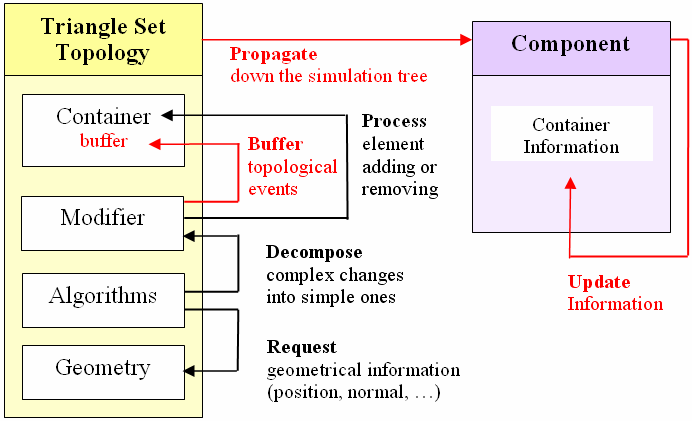
\includegraphics[width=0.7\textwidth]{topology/Handling_Changes}
    \caption{Handling topological changes, with the example of a {\em Triangle Set Topology}. 
    {\em Component} corresponds to any component of the simulation which may need topological information to perform a specific task.
    Black features indicate the effective change process. Red features show the steps of event notification.}
    \label{fig:Handling_Changes}
\end{figure}

\begin{figure}[ht]
 \centering
 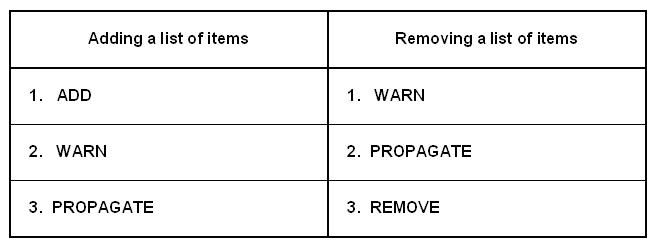
\includegraphics[width=0.65\linewidth]{topology/Order_Notifications}
  \caption{Order to respect when adding or removing an item. WARN means : add the current topological change (add or delete a list of items) in the list of TopologyChanges. PROPAGATE means :  traverse the simulation tree with a TopologyChangeVistor to send the current topological change event to all force fields, constraints, mappings, etc.}
 \label{fig:Order_Notifications}
\end{figure}


\begin{figure}[ht]
    \centering
        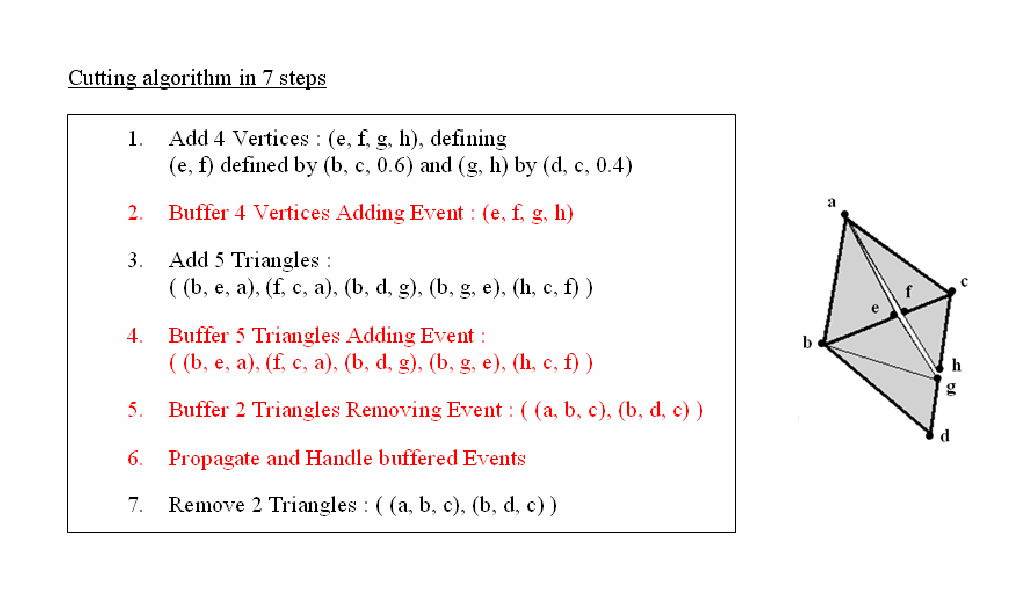
\includegraphics[width=0.8\textwidth]{topology/7_Steps_Cutting_Algorithm}
    \caption{Seven steps to perform cutting along two triangles (these generic steps would be the same to cut an arbitrarily number of triangles).
    Black steps indicate the effective change process. Red steps show the steps of event notification.}
    \label{fig:7_Steps_Cutting_Algorithm}
\end{figure}


The mechanism to handle topological changes is illustrated by Fig.~\ref{fig:Handling_Changes}.
The notification step consists in accumulating the sequence of
topological events  involved in a high-level topological change into a buffer stored in
the {\em Container}. Then the event list is propagated to all its
neighbors and leaves beneath by using a visitor mechanism, called a
{\em Topology Visitor}. Once a given component is visited, the topological
events are actually processed one by one and the data structure used to store mesh related information are automatically updated.

In practice, for each specific component ({\em e.g.} spring-mass mechanical component), a set of callback functions are provided describing how to update the data structure ({\em e.g.} spring stiffness and damping values) when adding or removing an element ({\em e.g.} the edges defined by the two extremities of the springs).
We applied the observer design pattern so that component-related data structures update themselves automatically.


\subsection{Combining Topologies}

Handling a single mesh topology in a surgery simulation scene is often too restrictive. There are at least three common situations where it is necessary to have, for the same mesh, several topological descriptions sharing the same degrees of freedom: the {\em boundary}, {\em composite} and {\em surrogate} cases. In the {\em boundary } scenario,  specific  
algorithms may be applied to the boundary of a mesh, the boundary of tetrahedral mesh being a triangulated mesh and that of a triangular mesh being a polygonal line. For instance, those algorithms may consist of applying additional membrane forces ({\em e.g.} to simulate the effect of the Glisson capsule in the liver) or visualizing a textured surface. Rather than designing specific simulation components to handle triangulations as the border of tetrahedrisations, our  framework allows us to create a triangulation topology object from  a tetrahedrisation mesh and to use regular components associated with triangulations.

The {\em composite} scenario consists in having a mesh that includes several types of elements: triangles with quads, or hexahedra with tetrahedra. Instead of designing specific components for those composite meshes, it is simpler and more versatile to reuse components that are dedicated to each mesh type. Finally the {\em surrogate} scenario corresponds to cases where one topological element may be replaced by a set of elements of a different type with the same degrees of freedom. For instance a quad may be split into two triangles while an hexahedron may be split into several tetrahedra. Thus a quad mesh may also be viewed as a triangular mesh whose topology is constrained by the quad mesh topology.

\begin{figure}[ht]
    \centering
        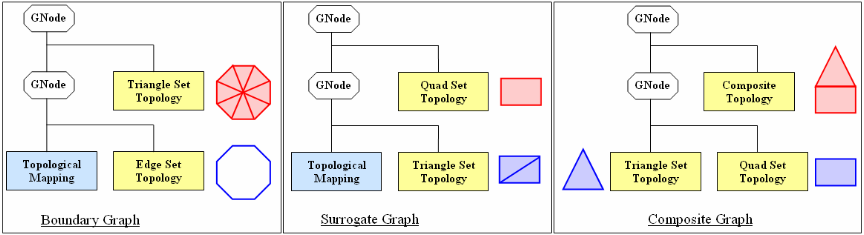
\includegraphics[width=1.0\textwidth]{topology/Combining_Topologies}
    \caption{Three scenari examples to combine topologies. ({\em From left to right}) A {\em Boundary Graph} from a triangle set to an edge set, a {\em Surrogate Graph} from a quad set to an triangle set and a {\em Composite Graph} superseding a quad set and a triangle set.}
    \label{fig:Combining_Topologies}
\end{figure}

These three cases can be handled seamlessly by using a graph of multiple topologies, the topology object being at the top node having the specific role of controlling the topologies below. Although we chose to duplicate topological information in memory, it has no effect on the time required to compute the forces.  Fig.~\ref{fig:Scene_Graph_TopologicalMapping} provides an example of a border scenario (triangulation as the border of a tetrahedralisation) while Fig.~\ref{fig:Combining_Topologies} shows general layout of topology graphs in the three cases described previously. In any cases, those graphs include a dedicated component called a {\em Topological Mapping} whose objectives are twofold. First, they translate topological events originating from the master topology ({\em e.g.} remove this quad) into topological actions suitable for the slave topology ({\em e.g} remove those two triangles for a surrogate scenario). Second, they provide index equivalence  between global numbering of elements in the master topology ({\em e.g} a triangle index in a tetrahedralisation topology ) and local numbering in the slave topology ({\em e.g} the index of the same triangle in the border triangulation). Possible {\em Topological Mappings} from a topology object to another have been represented by blue arrows in Fig.~\ref{fig:BW_Topology_Family_Tree}.

Note that those topology graphs can be combined and cascaded, for instance by constructing the triangulation border of a tetrahedrisation created from an hexahedral mesh.  But only topology algorithms of the master topology may be called to simulate cutting or to locally refine a volume. By combining topology graphs with generic components one can simulate fairly complex simulation scenes where topological changes can be seamlessly applied.


\subsection{An example of Topological Mapping : from TetrahedronSetTopology to TriangleSetTopology}

A TopologicalMapping is a new kind of Mapping which converts an
input topology to an output topology (both topologies are of type
BaseTopology).
\\

It first initializes the mesh of the output topology from the mesh
of the input topology, and it creates the two Index Maps that
maintain the correspondence between the indices of their common
elements.
\\

Then, at each propagation of topological changes, it translates the
topological change events that are propagated from the input
topology into specific actions that call element adding methods or
element removal methods on the output topology, and it updates the
Index Maps.
\\

So, at each time step, the geometrical and adjacency information are
consistent in both topologies.

Here is the scene-graph corresponding to the simulation of an object
which can be represented as a tetrahedral volume (on which one
volume force is applied) or as a triangular surface (on which two
surface forces are applied). Note that the Visual Model and the
Collsion Model are attached to the surface mesh of the object :


\begin{figure}[ht]
 \centering
 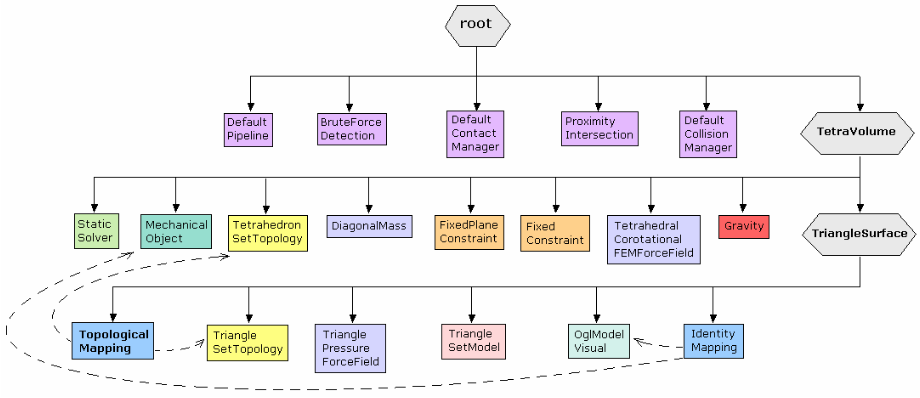
\includegraphics[width=1.0\linewidth]{topology/Scene_Graph_TopologicalMapping}
  \caption{Scene Graph illustrating a TopologicalMapping from a TetrahedronSetTopology to a TriangleSetTopology.}
 \label{fig:Scene_Graph_TopologicalMapping}
\end{figure}

Let us consider an example where the user wants to remove one tetraheron (whose one triangle at least is visible) from the tetrahedral volume.
The component Tetra$2$TriangleSetTopology handles this topological change by following five steps :
\\


\begin{itemize}

    \item \textbf{Step $1$.} The user right-clicks on visible triangle T in the scene, which is detected by the Collision Model and indexed by $loc\_T$ in the triangular surface mesh.
    
\begin{figure*}
 \centering
 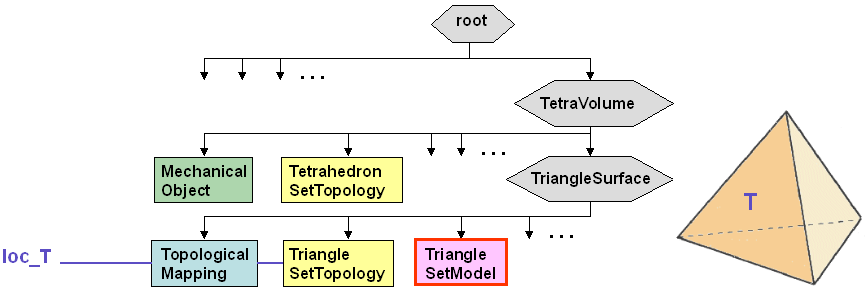
\includegraphics[width=1.0\linewidth]{topology/TopoMap_example_1}
  \caption{Scenario when the user wants to remove one tetraheron.- Step 1.}
 \label{fig:TopoMap_example_1}
\end{figure*}


    \item \textbf{Step $2$.} If a Topological Mapping of type ( input = TetrahedronSetTopology, output = TriangleSetTopology ) does exist, the index map $Loc2GlobVec$ is requested to give the index $glob\_T$ which is indexing the triangle T in the tetrahedral volume mesh. 
The TetrahedronTriangleShell gives then the index $ind\_TE$ which is indexing the unique tetrahedron TE containing T. 
We call the action RemoveTetrahedra($< ind\_TE >$) on the input topology.

\begin{figure*}
 \centering
 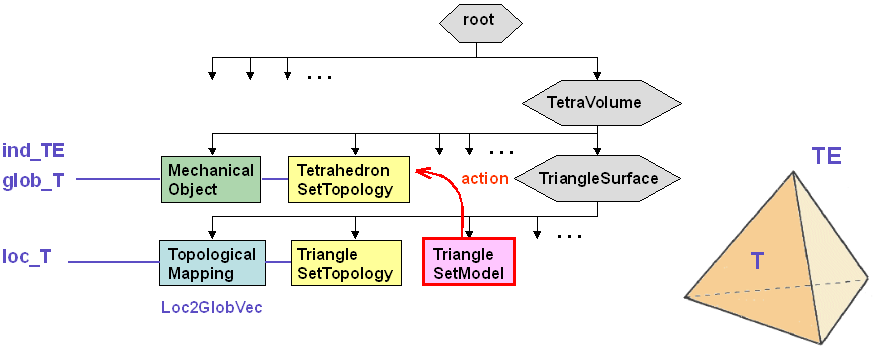
\includegraphics[width=1.0\linewidth]{topology/TopoMap_example_2}
  \caption{Scenario when the user wants to remove one tetraheron.- Step 2.}
 \label{fig:TopoMap_example_2}
\end{figure*}


    \item \textbf{Step $3$}. The TetrahedronSetTopology notifies all the removal events, that are successively concerning one tetrahedron, one or more isolated triangles, the possibly isolated edges and the possibly isolated points.

\begin{figure*}
 \centering
 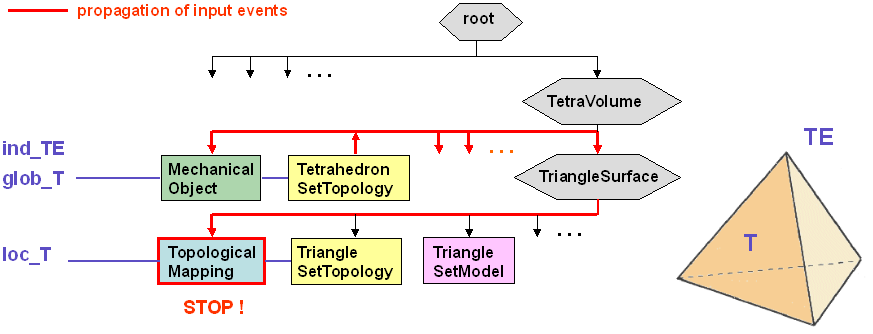
\includegraphics[width=1.0\linewidth]{topology/TopoMap_example_3}
  \caption{Scenario when the user wants to remove one tetraheron.- Step 3.}
 \label{fig:TopoMap_example_3}
\end{figure*}


    \item \textbf{Step $4$.} The propagation of topological events reaches a Topological Mapping which is strictly lower in the scene graph, then it stops.
The Tetra2TriangleTopologicalMapping translates the input events into output actions on the TriangleSetTopology.
The event Tetrahedron removal is translated into the action AddTriangles ( $<$ indices of new visible triangles $>$ ).
The event Triangle removal is translated into the action RemoveTriangles ( $<$ indices of destroyed triangles $>$, removeDOF $=$ false ), where (removeDOF $=$ false) indicates that the DOFs of the isolated points must not be deleted because they have already been removed by the input topology.
The Index maps ( Loc2GlobVec, Glob2LocMap, In2OutMap ) are requested and updated to maintain the correspondence between the items indices in input and output topologies.

\begin{figure*}
 \centering
 \includegraphics[width=1.0\linewidth]{topology/TopoMap_example_4}
  \caption{Scenario when the user wants to remove one tetraheron.- Step 4.}
 \label{fig:TopoMap_example_4}
\end{figure*}


    \item \textbf{Step $5$.} The adding events concerning one or more new visible triangles and the removal events concerning one or more isolated triangles are notified from the TriangleSetTopology.

\begin{figure*}
 \centering
 \includegraphics[width=1.0\linewidth]{topology/TopoMap_example_5}
  \caption{Scenario when the user wants to remove one tetraheron.- Step 5.}
 \label{fig:TopoMap_example_5}
\end{figure*}

\end{itemize}

\subsection{Example of scene file with a topological mapping}

\begin{figure*}
 \centering
 \includegraphics[width=0.9\linewidth]{topology/cylinder_example}
  \caption{Scene Graph simulating a bending cylinder as a tetrahedral volume and as a triangular surface (the cylinder membrane)}
 \label{fig:cylinder_example}
\end{figure*}

\newpage

Here is the scene file corresponding to the example :

\begin{verbatim}

<Node name="root" dt="0.05" showBehaviorModels="1" showCollisionModels="0" showMappings="0" 
 showForceFields="0" showBoundingTree="0" gravity="0 0 0">
  
	<Object type="CollisionPipeline" verbose="0" />
	<Object type="BruteForceDetection" name="N2" />
	<Object type="CollisionResponse" response="default" />
	<Object type="MinProximityIntersection" name="Proximity" alarmDistance="0.8" 
	 contactDistance="0.5" />
	
	<Object type="CollisionGroup" />

	<Node name="TT">
	
		<Object type="EulerImplicit" name="cg_odesolver" printLog="false"/>
		<Object type="CGLinearSolver" iterations="25" name="linear solver" tolerance="1.0e-9" 
		 threshold="1.0e-9" />
		
		<Object type="MeshLoader" name="meshLoader" filename="mesh/cylinder.msh" />
		<Object type="MechanicalObject" name="Volume" />
		<include href="Objects/TetrahedronSetTopology.xml" />

    <Object type="DiagonalMass" massDensity="0.5" />
		<Object type="FixedPlaneConstraint" direction="0 0 1" dmin="-0.1" dmax="0.1"/>
		<Object type="FixedConstraint" indices="0" />		
    <Object type="TetrahedralCorotationalFEMForceField" name="FEM" youngModulus="60" 
     poissonRatio="0.3" method="large" />
    
    <Object type="Gravity" gravity="0 0 0"/>

		<Node name="T">
		
			<include href="Objects/TriangleSetTopology.xml" />
			<Object type="Tetra2TriangleTopologicalMapping" object1="../../Container" object2="Container"/>

      <Object type="TriangularFEMForceField" name="FEM" youngModulus="10" poissonRatio="0.3" 
       method="large" /> 
			
			<Object type="TriangularBendingSprings" name="FEM-Bend" stiffness="300" damping="1.0"/>		
			    
			<Object type="TriangleSet"/>

			<Node name="Visu">
			
				<Object type="OglModel" name="Visual" color="blue" />
				<Object type="IdentityMapping" object1="../../../Volume" object2="Visual" />
				
			</Node>						
			
		</Node>
		
	</Node>
	
</Node>

\end{verbatim}

Here is the example of the included TriangleSetTopology.xml file, where the four members of the {\em TriangleSetTopology} are defined :

\begin{verbatim}

<Node name="Group"> 
  <Object type="TriangleSetTopologyContainer"  name="Container" />
  <Object type="TriangleSetTopologyModifier"   name="Modifier" />
  <Object type="TriangleSetTopologyAlgorithms" name="TopoAlgo"   template="Vec3d" />
  <Object type="TriangleSetGeometryAlgorithms" name="GeomAlgo"   template="Vec3d" />
</Node>

\end{verbatim}

\subsection{How to make a component aware of topological changes ?}

%%%

There are actually a few generic lines of code to add in a component for it to handle topological changes.
\\

If the component is based on topological elements like edges, the main idea is to introduce an object {\em edgeinfo} of type {\em EdgeData} 
and to template it by a data structure {\em EdgeInformation} that is attached to each edge (this data structure has to be defined by the component, to which it is specific).
By calling the method {\em handleTopologyEvents} on the object {\em edgeinfo} (of type {\em EdgeData} $<${\em EdgeInformation}$>$), the component-related data structure is automatically updated (code has been implement in file {\em EdgeData.inl}).
\\

Here : {\em edgeinfo}$[i]$ is the data structure attached to the edge indexed by $i$ in the topological component {\em EdgeSetTopology}.
\\

In SOFA, among the existing ForceField component able to handle topological changes there are for example : {\em BeamFEMForceField} (for the simple case) and {\em TriangularBendingSprings} (for the complicated case : data structure attached to each edge need to contain indices of points, which must also be updated by the method {\em handleTopologyChange}).
\\

For the simple case, here is how to adapt a Force Field component called {\em totoForceField} (for instance based on elements of type edge) to topological changes : 

\subsubsection{Modifications in header file {\em totoForceField.h} :}

\begin{itemize}

	\item Include the following header :  \begin{verbatim} #include <sofa/component/topology/EdgeData.h> \end{verbatim}
	
	\item Define a structure {\em EdgeInformation} which describes the information attached to each edge (for example {\em spring stiffness},
{\em spring length}, ...)
	
	\item Add an object {\em edgeinfo} of type {\em EdgeData} templated by the type
{\em EdgeInformation} : \begin{verbatim} topology::EdgeData<EdgeInformation> edgeinfo;  \end{verbatim}

	\item Declare the virtual method {\em handleTopologyChange} : \begin{verbatim} virtual void handleTopologyChange(); \end{verbatim}

  \item Add the callback function for the creation of edges :

\begin{verbatim} 

static void EdgeCreationFunction(
    int edgeIndex,
    void* param,
    EdgeInformation &ei,
    const topology::Edge& ,
    const sofa::helper::vector< unsigned int > &,
    const sofa::helper::vector< double >&
);


\end{verbatim} 

\end{itemize}

\subsubsection{Modifications in inline file {\em totoForceField.inl} :}


\begin{itemize}

	\item Add at the end of the method {\em init()} to specify the callbacks :
	
	\begin{verbatim} 

edgeinfo.setCreateFunction(EdgeCreationFunction);
edgeinfo.setCreateParameter( (void *) this );
edgeinfo.setDestroyParameter( (void *) this );

\end{verbatim} 
	
	\item Implement the method {\em handleTopologyChange()} :
	
  \begin{verbatim} 

template <class DataTypes>
void totoForceField<DataTypes>::handleTopologyChange()
{

    std::list< const sofa::core::componentmodel::topology::TopologyChange* >
::const_iterator itBegin = _topology->firstChange();

    std::list< const sofa::core::componentmodel::topology::TopologyChange*>
::const_iterator itEnd = _topology->lastChange();

    edgeinfo.handleTopologyEvents(itBegin,itEnd);
    
}
\end{verbatim} 

	\item Implement the method {\em EdgeCreationFunction} (usefull for the initialization of the data attacheed to a new edge) :
	
	\begin{verbatim} 
	
template<class DataTypes>
void totoForceField<DataTypes>::EdgeCreationFunction(

int edgeIndex, void* param, EdgeInformation &ei,
const topology::Edge& e,  const sofa::helper::vector< unsigned int > &a,
const sofa::helper::vector< double >&
)

{

    totoForceField<DataTypes> *ff= (totoForceField<DataTypes> *)param;

    if (ff) {

      ei.champ = value; // initialiser tous les champs de "edgeinfo[i]"

      (...)

    }
}
	
	\end{verbatim} 
	
	
\end{itemize}

At any time, it is possible to access the information from the container member of the topology (so as to get some neighborhood information) by using a pointer to the {\em BaseMeshTopology} API :

	\begin{verbatim} 
	
sofa::core::componentmodel::topology::BaseMeshTopology* _topology;
_topology = getContext()->getMeshTopology();

	\end{verbatim} 


\subsection{What happens when I split an Edge ?}

\begin{figure*}[htpb]
 \centering
 \includegraphics[width=0.9\linewidth]{topology/Topology_Example_1}
 \includegraphics[width=0.9\linewidth]{topology/Topology_Example_2}
  \caption{What happens when I split an Edge ? - Step 1. 2.}
 \label{fig:Topology_Example_12}
\end{figure*}

\newpage

\begin{figure*}[htpb]
 \centering
 \includegraphics[width=0.9\linewidth]{topology/Topology_Example_3}
 \includegraphics[width=0.9\linewidth]{topology/Topology_Example_4}
  \caption{What happens when I split an Edge ? - Step 3. 4.}
 \label{fig:Topology_Example_34}
\end{figure*}

\newpage

\begin{figure*}[htpb]
 \centering
 \includegraphics[width=0.9\linewidth]{topology/Topology_Example_5}
 \includegraphics[width=0.9\linewidth]{topology/Topology_Example_6}
  \caption{What happens when I split an Edge ? - Step 5. 6.}
 \label{fig:Topology_Example_56}
\end{figure*}

\newpage

\begin{figure*}[htpb]
 \centering
 \includegraphics[width=0.9\linewidth]{topology/Topology_Example_7}
 \includegraphics[width=0.9\linewidth]{topology/Topology_Example_8}
  \caption{What happens when I split an Edge ? - Step 7. 8.}
 \label{fig:Topology_Example_78}
\end{figure*}

\newpage

\begin{figure*}[htpb]
 \centering
 \includegraphics[width=0.9\linewidth]{topology/Topology_Example_9}
  \caption{What happens when I split an Edge ? - Step 9.}
 \label{fig:Topology_Example_9}
\end{figure*}

               
% \subsubsection{Use Cases}

%%%%%%%%%%%%%%%%%%%% COMPONENTS%%%%%%%%%
%1 STATES
\chapter{States}
\graphicspath{{../states/}}  % to include images
\input{../states/states}


%2 MECA FORCES
\chapter{Mechanical forces}
\emph{to be completed}
\section{ForceField components}

\section{Interaction ForceField}
\label{sec:interactionforcefield}

\section{Mass and inertial forces}

%3 MAPPING
\chapter{Mappings}
\input{../mappings/mappings_body}
\section{Barycentric Mapping}
\section{Rigid Mapping}
\section{Identity Mapping}
\section{Skinning Mapping}


%4 SOLVERS
\chapter{Solvers}
\label{chap:solvers}
\graphicspath{{../solvers/}} 
\section{ODE solvers} 

ODE solvers implement animation algorithms applied at each time step to integrate time and compute positions and velocities one time step forward in time.
% Each step of the algorithm is implemented using a visitor to traverse the scenegraph starting from the node the solver is attached to.
The solvers do not directly address the physical models. 
They apply abstract mechanical operations to state vectors represented by IDs, as illustrated in the algorithm shown in Figure~\ref{fig:eulerexplicit}.
\begin{figure}
\begin{center}
\begin{algorithmic}
\STATE void  \textbf{ExplicitEulerSolver::solve(VecId x, VecId v, double dt)}
\STATE create auxiliary vectors a,f
\STATE resetForce(f)
\STATE accumulateForce(f,x,v)
\STATE computeAcceleration(a,f)
\STATE project(a,a)
\STATE v += a * dt
\STATE x += v * dt
\end{algorithmic}
\caption{Euler's explicit time integration.}
\label{fig:eulerexplicit}
\end{center}
\end{figure}
Each mechanical operation, such as allocating a state vector or accumulating the forces, is implemented using a specialized visitor parameterized on vector IDs or control values such as dt.
This allows to implement the solvers completely independenly of the physical model.
Each vector used by a solver ID is actually scattered over all the state vector containers in the different nodes in the scope of the solver.
Some vector operations such as the dot product apply only to the independent DOFs, stored in the state vectors not attached to a parent by a mapping.
Notice that this design avoids the assembly of global state vectors (i.e. copying Vec3 and quaternions to and from  vectors of scalars).
Moreover, the virtual function calls are resolved at the granularity of the state vectors (i.e. all the particles together, and all the moving frames together) rather than each primitive (i.e. each particle and each frame independently), and allow to optimize each implementation independently.
There is thus virtually no loss of efficiency when mixing arbitrary types in the same simulation.




% The ODE solver creates visitors and applies them to its parent node.
% The ComputeDf visitor presented in Figure~\ref{fig:DfVisitor} finds no mapping nor DOF at the root level (functions are called only if the corresponding component is present in the node), and continues the traversal in the two child branches. 
% Each object computes its own force change df corresponding to its own displacement dx, as previously explained.
% The objects are independent because there is no mapping to a commom DOF component at the scene level.
% Each object manages its own state vectors.
% Thus, using visitors allows the solver to transparently handle an arbitrary number of objects of arbitrary types in the same scene. 
% One can use visitors without knowing to which objects they apply.
% This is a key feature of the SOFA design, which allows us design the algorithms once and to apply them to all types of simulated objects.
% Notice that this design avoids the assembly of global state vectors (i.e. copying Vec3 and quaternions to and from  vectors of scalars).
% Moreover, the virtual function calls are resolved at the granularity of the state vectors (i.e. all the particles together, and all the moving frames together) rather than each primitive (i.e. each particle and each frame independently), and allow to optimize each implementation independently.
% There is thus virtually no loss of efficiency when mixing arbitrary types in the same simulation.
% Hence the ``versatile yet efficient'' motto of SOFA.


We have identified two families of ODE solvers.
The first contains the explicit solvers, which compute the derivative at the beginning of the time step. They are variants of the Euler explicit solver presented in Figure~\ref{fig:eulerexplicit}, and are easily implemented in Sofa using the same operators.
The second family contains the implicit solvers, which consider the derivative at the end or somewhere in the middle of the time step. They typically require the solution of equation systems such as:
\begin{equation}
\label{eq:linear-system}
\underbrace{\left(\alpha \M  + \beta \B  + \gamma \K \right)}_{\mathbf{A}}   \Vdv =  \vec b
%\underbrace{\P \left(\alpha \M  + \beta \B  + \gamma \K \right)}_{\mathbf{A}}   \Vdv =  \vec b
\end{equation}
where $\M$ is the mass matrix, $\K = \frac{\partial \Vf}{\partial \Vx}$ and $\B = \frac{\partial \Vf}{\partial \Vv}$ respectively are the \textit{stiffness} and \textit{damping} matrices (the method is explicit if $\beta$ and $\gamma$ are null). In order to apply simple displacement constraints,  a projection matrix $\P$ can be used, and the system becomes $\P^T \mathbf{A} \P \Vdv =\P^T \vec b $~\cite{baraff98large}.
Implicit integration has the advantage of being more stable for stiff forces or large time steps. However, solving these equation systems requires linear solvers, discussed in the next section.
Currently, eight ODE solvers have been implemented, including symplectic Euler and explicit Runge-Kutta4, implicit Euler and statics solution.



\section{Linear solvers} 
\subsection{Conjugate Gradient} An interesting feature of visitor-based mechanical computations is their ability to efficiently and transparently compute matrix products.
Thus, we have proposed in SOFA an implementation of the Conjugate Gradient, based on the graph traversal. 
The visitor shown in Figure~\ref{fig:DfVisitor} computes the force change \textit{df} based on a given displacement \textit{dx}, as repeatedly performed in Conjugate Gradient algorithm. 
An arbitrary number of forces and projections may be present in all the nodes, resulting in a complicated stiffness matrix, as shown in the following equation:
\begin{equation}
 \label{eq:dfdx}
\vec{df} = \sum_i  \left( \prod_{j \in path(i)} \mat J_j  \right)^T \K_i \left( \prod_{j \in path(i)} \mat J_j  \right) \vec{dx}
\end{equation}
where $\K_i$ is the stiffness matrix of force $i$, matrix $\J$ encodes the first-order mapping relation of a node with respect to its parent, and $path(i)$ is the list of nodes from the solver to the node the force applies to.
\begin{figure}
\begin{center}
\begin{tabular}{c|c}
\begin{minipage}[t]{0.52\linewidth}
\begin{algorithmic}
\STATE bool \textbf{ComputeDfVisitor::topDown}():
\STATE dof.resetF(this.df)
\IF{mapping}
\STATE mapping.applyJ(this.dx)
\ENDIF
% \FORALL {projection P}
% \STATE P.project( this.dx,this.dx )
% \ENDFOR
\RETURN true
\end{algorithmic}
\end{minipage}
&
%  \hspace{0.01\linewidth}
% &
%  \hspace{0.01\linewidth}
% &
 \begin{minipage}[t]{0.46\linewidth}
\begin{algorithmic}
\STATE void \textbf{ComputeDfVisitor::bottomUp}():
\FORALL {forceField F}
\STATE F.addDF( this.df,this.dx )
\ENDFOR
% \FORALL {projection P}
% \STATE P.project( this.df,this.df )
% \ENDFOR
\STATE mapping.applyJT(this.df)
\end{algorithmic}
 \end{minipage}
\end{tabular}
\caption{Computing $df$ given $dx$ using a visitor.}
\label{fig:DfVisitor}
\end{center}
\end{figure}
This complex product is computed using only matrix-vector products and with optimal factoring thanks to the recursive implementation.
It allows us to efficiently apply implicit time integration to arbitrary scenes using the Conjugate Gradient. 
This method allows us to trade-off accuracy for speed by limiting the number of steps of the iterative solution.


\subsection{Direct Solvers} Direct solvers are also available in SOFA. They can be used as preconditionners of the conjugate gradient algorithm~\cite{CADC10} or for directly solving equation \ref{eq:linear-system}.
Their implementation are based on external libraries such as Eigen, MKL and Taucs. 
When dealing with Finite Element Models, the matrices are generally very sparse and 
efficient implementations based on sparse factorizations allow for fast computations. 
Moreover, when dealing with specific topologies, like wire-like structures, tri-diagonal band solvers can be used for extremely fast results in $\mathcal{O}(n)$
These different linear solvers address matrices which  can be stored in different formats, adapted to the numerical library.
%or even not explicitly stored when only matrix-vector products are applied.
The type of matrix is a parameter of the linear solver, and of the visitors the solver uses. 
Ten linear solvers have been implemented in \sofa{}. They can be interchanged to compare their efficiency.

\subsection{From ODE solver to linear solver}

In SOFA, all states of a mechanical object is described by its degree of freedom. The main works for the simulation are filling and inverting a matrix system in order to find the states of mechanical objects by steps of time. This system matrix can be described as below :
 \[
\left[ \textbf{MBK} \right].a=f \text{    ,  or at time n+1 :   }\left[ \textbf{MBK} \right].a_{n+1}=f_{n+1}
\]
where,
\[
\left\{ 
\begin{array}{l}
\textbf{M} \text { : the mass matrix   }  \\
\textbf{B} \text { : the damping matrix   }  \\
\textbf{K} \text { : the stiffness matrix   }  \\
\left[ \textbf{MBK} \right] \text {  : is a linear combination of MBK (not multiplication)   }  \\
a_{n+1} \text { : accelerator field} \\
f_{n+1} \text { : force field} 
\end{array}\right.
\]
 Usually, \textbf{M} is filled by \textbf{mass} components, \textbf{K} is filled by \textbf{forcefield} or \textbf{interactionforcefield} components, \textbf{B} (often $\alpha\textbf{M}+\beta\textbf{K}$ ) and $\left[ \textbf{MBK} \right]$ are computed by \textbf{odesolver} components. The works left to invert the matrix system are done by \textbf{linearsolver} components.
\begin{center}
\includegraphics[scale=0.3]{matrix_bloc.pdf}
\end{center}
On the case for example when there are two mechanical objects, we can see a global stiffness matrix describing the two mechanical states, composed diagonal blocs and non-diagonal blocs. The diagonal blocs are filled by \textbf{mass},\textbf{forcefield} components, and the non-diagonal ones are filled by \textbf{interactionforcefield} if existed.
\paragraph{Mapping matrix contribution : } When existe a mapping on the simulation scene, the states of two mechanical objects are relied by : 
\[
\begin{array}{rl}
\textbf{x}_{2} & = \Im\left(\textbf{x}_{1}\right)           \text{      ,	mapping::apply}             \\
\textbf{v}_{2} & = \left[\textbf{J}\right] \textbf{v}_{1}   \text{      ,	mapping::applyJ}  
\end{array}
\]
The $\left[\textbf{J}\right]$ matrix is derivative of $\Im$ operator and is defined by the \textbf{mapping} components. The dynamic and matrix system of the two objects are relied by :   
\[
\begin{array}{rl}
\textbf{f}                  & += \textbf{f}_{1}  +   \left[\textbf{J}\right]^{t} \textbf{f}_{2}         \text{      ,	mapping::applyJT}             \\
\left[ \textbf{MBK} \right] & += \left[ \textbf{MBK} \right]_{1}  + \left[\textbf{J}\right]^{t}  \left[ \textbf{MBK} \right]_{2} \left[\textbf{J}\right]
\end{array}
\]
The resolution of the system with the mapping is done in general :
\[
\left\{ 
\begin{array}{rl}
\textbf{a}^{n+1}        & = \left[ \textbf{MBK} \right]^{-1}  \textbf{f}^{n+1}    \\
\textbf{v}^{n+1}_{1}    & = \textbf{v}^{n}_{1}     + dt.\textbf{a}^{n+1}         \\
\textbf{x}^{n+1}_{1}    & = \textbf{x}^{n}_{1}     + dt.\textbf{v}^{n+1}         \\
\textbf{x}^{n+1}_{2}    &  \text{ ,	mapping::apply }     \\
\textbf{v}^{n+1}_{2}    &  \text{ ,	mapping::applyJ }          
\end{array}
\right.
\]



\subsection{Particular implementation in SOFA}
The direct solver demands to build explicitly the matrix, and invert this matrix after every step of time in order to solve the mechanical response after a solicitation. In SOFA, there are a little more complicated component called mapping, relying geometrical and mechanical properties by master-slave (DOF-mapped object) relation. All changes of geometry or solicitation to one object interfere to other and vice versa. If the mapped object have its own mechanical behavior, it must be counted on the mechanical propagation by the mapping.
\subsubsection{self-stiffness propagation }
\[
\begin{array}{cc}
\includegraphics[scale=0.3]{stiffness_propagation_matrix.pdf}        
& 
\includegraphics[scale=0.35]{stiffness_propagation.pdf} 
\end{array}
\]
In the simple simulation scene, \textbf{MS2} is a mapped object to the \textbf{MS1} mechanical object by the mapping. The matrix to be inverted for all mechanical response is the filled colorized one ($K_{11}$), the matrix $K_{22}$ describing mechanical properties of the second objects must contribute to $K_{11}$ by the formula :
\[
\left\{ 
\begin{array}{ll}
K_{11}       & += J^t * K_{22} * J               \\
\text{or,}   &         \\
K_{tempo}    & =  J^t * K_{22}                   \\
K_{11}       & += K_{tempo} * J                  \\         
\end{array}
\right.
\]
By doing this computation, we propagate the stiffness of the mapped mechanical object to its root mechanical object.
\subsubsection{interaction-stiffness propagation }
In the general case, the may have a simulation scene where there are many level of mapped mechanical states (mapped of mapped state ...) and many interaction forcefield interacting between them. Therefor the stiffness of interaction forcefield and the mapped mechanical state need to be propagated through the mappings. We can imagine for one propagation, there are two simple cases.
\paragraph{Interaction beweent Real Mechanical Object and Mapped Mechanical Object}
\[
\begin{array}{cc}
\includegraphics[scale=0.3]{interaction_Real_Mapped_Matrix}        
& 
\includegraphics[scale=0.35]{interaction_Real_Mapped} 
\end{array}
\]
In the case where one of the two mechanical states in interaction is non-mapped, the propagation can be computed directly by the formula :
\[
\left\{ 
\begin{array}{ll}
K_{11}       & += J^t * K_{33} * J               \\
\text{or,}   &                                   \\
K_{tempo}    & =  J^t * K_{33}                   \\
K_{11}       & += K_{tempo} * J                  \\ 
\text{and,}&                 \\      
I_{12}       & += J^t * I_{32}                   \\ 
I_{21}       & += I_{23} * J                        
\end{array}
\right.
\]
\paragraph{Interaction beweent Mapped Mechanical Object and Mapped Mechanical Object}
\begin{center}
  \includegraphics[scale=0.3]{interaction_Mapped_Mapped}
\end{center}
In the case where the two mechanical states in interaction are mapped, the propagation can be computed by two steps. The first consist to propagate the interaction $I_{34}$ to the interation $I_{14}$ :
\[
\left\{ 
\begin{array}{ll}
K_{11}       & += J^t * K_{33} * J               \\
\text{or,}   &                                   \\
K_{tempo}    & =  J^t * K_{33}                   \\
K_{11}       & += K_{tempo} * J                  \\ 
\text{and,}&                 \\      
I_{14}       & += J^t_A * I_{34}                  \\ 
I_{41}       & += I_{43} * J_A                        
\end{array}
\right.
\]
The following step can compute as the one of above paragraph, propagating the interation $I_{14}$ to $I_{12}$.


%In summary, ODE solution is performed using a hierarchy of algorithms and data structures with each level implemented in a different component: the main ODE solution algorithm , the auxiliary linear solver  parameterized by the type of matrix, and an optional preconditioner when the Conjugate Gradient linear solver is used.
%Using a direct solver requires the explicit computation and storage of the system matrix \mat A of Equation~\ref{eq:linear-system}.
%The mass and stiffness matrices are written by the components and summed at each node level. They are then multiplied by the projection and mapping matrices during visitor traversals, and stored in the solver.

\section{Constraint solvers} 
\label{lm}
To handle different kinds of interactions (contact, friction, joints between particles..) between the simulated objects, SOFA allows the use of Lagrange multipliers~\cite{DDKA06}. 
%see \textit{e.g.}\cite{Duriez_eurographics2008}.
%The third family of solvers involves non-trivial constraints requiring additional equations, and additional unknowns called 
They may be combined with explicit or implicit integration.
Each constraint depends on the relative position of the interacting objects, and on optional parameters 
(such as a friction coefficient, etc.)\footnote{For simplicity, we present the equations for two interacting objects 
(rigid or deformable) $1$ and $2$, but the solution applies to arbitrary number of interacting bodies.}:
\begin{equation}
\begin{array}{c}
\Phi(\Vx_1, \Vx_2, ...) = 0 \\ 
\Psi(\Vx_1, \Vx_2, ... ) \geq 0
\end{array}
\label{eq:constraints}
\end{equation} where $\Phi$ represents the bilateral interaction laws (attachments, sliding joints, etc.) whereas $\Psi$ represents unilateral interaction laws (contact, friction, etc.). These functions can be non-linear.
% The solution uses Lagrange multipliers and a single linearization by time step (see~\cite{DDKA06}). 
The Lagrange multipliers are computed at each simulation step.
%However, for interaction including deformations, there is often a temporal coherency on the multipliers values. 
%Thus, we can provide an estimate $\tilde{\lambda}$ at the beginning of each time step and compute a correction $\Delta \lambda$ so that $\lambda = \tilde{\lambda} +\Delta \lambda$.  
They add force terms to Equation (\ref{eq:linear-system}):
\begin{equation}
\begin{array}{c}
\mathbf{A}_1  \Vdv_1 = \mathbf{b}_1 + \mathbf{H}_1^T \lambda\\
\mathbf{A}_2  \Vdv_2 = \mathbf{b}_2 + \mathbf{H}_2^T \lambda
\label{eq:constraint-systeme}
\end{array}
\end{equation}
where 
\begin{equation}
\mathbf{H}_1 = [\frac{\delta \Phi}{\delta \Vx_1} \  ; \  \frac{\delta \Psi}{\delta \Vx_1}  ]\qquad  \mathbf{H}_2 = [\frac{\delta \Phi}{\delta \Vx_2} \  ; \  \frac{\delta \Psi}{\delta \Vx_2}  ].
\end{equation}
Matrices $\mathbf{H}_1$ and $\mathbf{H}_2$ are stored in the mechanical state component of each node. Thus, when the constraint applies to a model that is mapped (see section \ref{sec:mappings}), the constraints are recursively mapped upward like forces to be applied to the independent degrees of freedom~\cite{Duriez_eurographics2008}. 
% An example that illustrates this concept can be found in \cite{Duriez_eurographics2008}. 
Solving the constraints is done by following these steps:


\textbf{Step 1, Free Motion}: interacting objects are solved independently while setting $ \lambda  = 0$. 
We obtain what we call a \textit{free motion} $\Vdv_1^{\mathrm{f}}$  and  $\Vdv_2^{\mathrm{f}}$ for each object. After integration, we obtain $\Vx_{1}^{\mathrm{f}}$ and $\Vx_{2}^{\mathrm{f}}$. 
%For the prediction, use $\tilde{\lambda} = \lambda^{t}$. 
During this step, each object solves equation~(\ref{eq:constraint-systeme}) with $ \lambda  = 0$ independently using a dedicated solver.  

\vspace{2mm}

\textbf{Step 2, Constraint Solving}: 
%the constraint laws are linearized as follows:
%\begin{equation}
%\label{eq:const-lin}
%\underbrace{
%\left[ \! \! \!
%\begin{array}{c}
%\Phi(\Vx_{1}^{t+h}, \Vx_{2}^{t+h})  \\
%\Psi(\Vx_{1}^{t+h}, \Vx_{2}^{t+h}) 
%\end{array} \! \! \!
%\right]}_{\boldsymbol{\delta}^{t+h}}  \! 
%=  \! 
%\underbrace{
%\left[ \! \! \!
%\begin{array}{c}
%\Phi(\Vx_{1}^{\mathrm{f}}, \Vx_{2}^{\mathrm{f}})  \\
%\Psi(\Vx_{1}^{\mathrm{f}}, \Vx_{2}^{\mathrm{f}}) 
%\end{array}\! \! \!
%\right]}_{\boldsymbol{\delta}^{\mathrm{f}}}
% + h\mathbf{H}_1\Vdv_1^{\mathrm{c}}  +  h\mathbf{H}_2\Vdv_2^{\mathrm{c}}
%\end{equation}
%With $\Vdv_1^{\mathrm{c}}$ and $\Vdv_2^{\mathrm{c}}$ being the unknown corrective motion ($\Vdv= \Vdv^{\mathrm{f}} + \Vdv^{\mathrm{c}}$) when solving equation \ref{eq:constraint-systeme} with $\mathbf{b}_1 = \mathbf{b}_2 = 0$. By gathering equations \ref{eq:constraint-systeme} and \ref{eq:const-lin}, we have:
The constrained equations can be linearized and linked to the dynamics (see \cite{CJADLC10} for details). 
\begin{equation}
\left[
\begin{array}{c}
\Phi(\Vx_{1}, \Vx_{2})  \\
\Psi(\Vx_{1}, \Vx_{2}) 
\end{array} \! \! \!
\right]
 =
 % \underbrace{
\left[ \! \! \!
\begin{array}{c}
\Phi(\Vx_{1}^{\mathrm{f}}, \Vx_{2}^{\mathrm{f}})  \\
\Psi(\Vx_{1}^{\mathrm{f}}, \Vx_{2}^{\mathrm{f}}) 
\end{array}\! \! \!
\right]
%}_{ \delta^{\mathrm{f}}  }
 + 
 \underbrace{
 h\mathbf{H}_1\Vdv_1^{\mathrm{c}}  +  h\mathbf{H}_2\Vdv_2^{\mathrm{c}}
 }_{h \left[  \mathbf{H}_1 \mathbf{A}_1^{-1}  \mathbf{H}_1^T + \mathbf{H}_2 \mathbf{A}_2^{-1}  \mathbf{H}_2^T \right]\lambda
 }
 %=
 %\delta^{\mathrm{f}} +
%\underbrace{h \left[  \mathbf{H}_1 \mathbf{A}_1^{-1}  \mathbf{H}_1^T + \mathbf{H}_2 \mathbf{A}_2^{-1}  \mathbf{H}_2^T \right]}_{\mathbf{W}} \lambda
\label{eq:addjminvjt}
\end{equation}
With $\Vdv^{\mathrm{c}} = \Vdv - \Vdv^{\mathrm{f}}$. 
Together with equation (\ref{eq:constraints}), these equations compose a Mixed Complementarity Problem that can be solved by a variety of solvers.
We compute the value of $ \lambda$ using a projected Gauss-Seidel algorithm that iteratively checks and projects the various constraint laws contained in $\Phi$ and  $\Psi$ ~\cite{DGMCG09}. 

\textbf{Step 3, Corrective Motion}: when the value of $\lambda$ is available, the corrective motion is computed as follows:
%
\begin{equation}
\label{eq:corrective-motion}
\begin{array}{c}
\Vx_{1}^{t+h} =  \Vx_{1}^{\mathrm{f}} + h \Vdv_1^{\mathrm{c}} \  \  \mathrm{ with } \  \  \Vdv_1^{\mathrm{c}} = \mathbf{A}_1^{-1}  \mathbf{H}_1^T \lambda \\
\Vx_{2}^{t+h} =  \Vx_{2}^{\mathrm{f}} + h \Vdv_2^{\mathrm{c}} \  \  \mathrm{ with } \  \  \Vdv_2^{\mathrm{c}} = \mathbf{A}_2^{-1}  \mathbf{H}_2^T \lambda
\end{array}
\end{equation}
%

A Master Solver, which is generally placed at the top of the graph of SOFA has the role of imposing this new scheduling to the rest of the graph. 
%
\begin{figure}[!htb]
\centering
% FreeMotionScheme is missing from SVN
\includegraphics[width= 0.9\columnwidth]{ConstraintSolver.png}
\caption{Contact process using constraints: A unilateral constraint is placed at the level of the contact points. The constraint direction is mapped to the degrees of freedom of the objects to obtain matrix $ \mathbf{H}^T$. The \textit{ConstraintCorrections} components compute the compliance to obtain equation \ref{eq:addjminvjt}. The Constraint solver found a new value of $\lambda$ which is sent to the  \textit{ConstraintCorrections} to compute an adequate corrective motion. The Master Solver is placed at the root of the simulation graph to impose the steps of the simulation process.  }
\label{shema_ToH}
\end{figure}

\textbf{Compliance computation} : Equations~\ref{eq:addjminvjt} and~\ref{eq:corrective-motion} involve the inverse of matrix $\mathbf{A}$ (called compliance matrix), which changes at every time step namely in case of a non-linear model. 
Depending on the simulation case, computing this inverse could be time consuming for real-time simulation. 
When this is too time-consuming, we propose several strategies to improve the speed of the algorithm such as using the diagonal of $\mathbf{A}$ instead of the hole matrix, or a precomputed inverse~\cite{Saupin08}, or an asynchronous factorization on the GPU~\cite{CourtecuisseMICCAI11}.  
These strategies are implemented in a category of components, called  \textit{ConstraintCorrections} that provide different ways of computing $\Vdv^{\mathrm{c}}$ given a value of $\lambda$. Given a simulation, it is very easy to make tests and chose the better solution.








%5 COLLISION
\chapter{Collision detection}
\graphicspath{{../collision/}} 
Collision detection is split in several phases, each implemented in a different component, and organized using a collision pipeline component.
Each potentially colliding object is associated with a collision geometry based on or mapped from the independent DOFs.
The broad phase component returns pairs of colliding bounding boxes (currently, axis-aligned bounding boxes).
Based on this, the narrow phase component returns pairs of geometric primitives with the corresponding collision points.
%\ff{Several collision detection approaches have been implemented: distances between pairs of geometric primitives (triangles and spheres), points in distance fields, distances between colliding meshes using ray-tracing~\cite{HerFauRaf08}, and intersection volume using images as sketched in Section~\ref{sec:LDI}.}
This is passed to the contact manager, which creates contact interactions of various types based on customizable rules.
Repulsion has been implemented based on penalties or on constraints using Lagrange multipliers, and is processed by the solvers together with the other forces at the next time step.
%If topological changes such as cutting operations are triggered, they are handled by the topology algorithms discussed in Section~\ref{sec:topologicalChanges}.
This framework has allowed us to efficiently implement popular proximity-based repulsion methods as well as novel approaches based on ray-casting~\cite{HerFauRaf08} or surface rasterization~\cite{FauBarAllFal08,AFCFDK10}.
Its main limitation is that the contacts can be mechanically processed only after they all have modeled by the collision pipeline.
This does not allow to mechanically react to a collision as soon as it is detected, possibly avoiding further collisions between primitives of the same objects.

When stiff contact penalties or contact constraints are created by the contact manager, an additional \textit{GroupManager} component is used to create interaction groups handled by a common solver, as discussed in Section~\ref{sec:scenes}. 
When contacts disappear, interaction groups can be split to keep them as small as possible.
The scenegraph structure thus changes along with the interaction groups.


\vspace{1cm}
\emph{to be completed}


%6 VISUAL
\chapter{Visual Rendering}


%7 HAPTIC
\chapter{Haptic Rendering}
\label{chap:haptic}
\graphicspath{{../haptic/}} 
The main interest of interactive simulation is that the user can modify the course of the computations in real-time.
This is essential for surgical simulation : during a training procedure, when a virtual medical instrument comes into contact with some models of a soft-tissue, \emph{instantaneous} deformations must be computed.
This visual feedback of the contact can be enhanced by haptic rendering so that the surgeon can really "feel" the contact.

There are two main issues for a platform like SOFA for providing haptic: The first is that haptic forces need to be computed at $1kHz$ whereas real-time visual feedback (without haptic) is obtained at $30Hz$. The second is that haptic feedback can add artificially some energy inside the simulation and can create instabilities, if the control is not \emph{passive}. 

Thus two different approaches are currently implemented into SOFA. The first one is the \emph{Virtual Coupling} technique and the other, more advanced, allows for rendering the constraints presented in section \ref{lm}.



\section{Virtual Coupling} Plugging of a haptic device is bidirectional: the user applies some motions or some forces on the device and this device, in return, applies forces and/or motions to the user.
The majority of the haptic devices propose a \emph{Impedance} coupling: the position of the device is provided by the API and this API asks for force values from the application.
A very simple scheme of coupling, presented in Fig\ref{fig:haptic1}, could have been used.
In this \emph{Direct coupling} case, the simulation would play the role of a controller in an open loop. 

\begin{figure}
\centering
 \includegraphics[width=0.7\linewidth]{haptic1.png}
 \caption{Direct coupling}
 \label{fig:haptic1}
\end{figure}

Such design is not suitable when stable and robust haptic feedback on a virtual environment is desired. Indeed some combination of the environment impedance and human user reactions can destabilize the system \cite{Adams99}. 
To avoid this, a virtual mechanical coupling is set. It corresponds to the use of a damped-stiffness between the position measured on the device and the simulated position in the virtual environment (see Fig\ref{fig:haptic2}). If very stiff constraints are being simulated then, the stiffness perceived by the user will not be infinite but will correspond to the stiffness of this virtual coupling. 
Hence, a compromise between stability and performance must be found by tuning the stiffness value of the coupling.

\begin{figure}
\centering
 \includegraphics[width=\linewidth]{haptic2.png}
 \caption{Virtual coupling technique. A 6 DoFs Damped spring is placed between the haptic loop and the simulation.}
 \label{fig:haptic2}
\end{figure}

The damped spring is simulated two times. One time in the haptic loop and one time in the simulation loop. 
If the two loops are synchronized, then the result is the same. But it can also be used in asynchronous mode: fast update of the haptic loop and low rates in the simulation.
In such case, the haptic feedback remains stable but the delay between the two loop is creating an artificial damping.
There is an option to cancel this artificial damping if no contact is detected in the simulation. However, this option can create a sensation of sticking contacts. 
The main advantage of the virtual coupling technique is that it can be easily employed with every simulation of SOFA. The main drawback is that the haptic rendering is not transparent.
 
\section{Constraint-based rendering} An innovative way of dealing with haptic rendering for medical simulation has been proposed in the context of SOFA (see\footnote{The implementation of  \cite{Saupin08} is available in open-source, for the implementation of \cite{Peterlik11}, please contact: christian.duriez@inria.fr }  \cite{Saupin08} and \cite{Peterlik11}). 
The approach deals with the mechanical interactions using appropriate force and/or motion transmission models named \emph{compliant mechanisms} (see Fig\ref{fig:haptic3}). 
These mechanisms are formulated as a constraint-based problem (like presented in section \ref{lm}) that is solved in two separate threads running at different frequencies. 
The first thread processes the whole simulation including the soft-tissue deformations, whereas the second one only deals with computer haptics. 
With this approach, it is possible to describe the specific behavior of various medical devices while relying on a unified method for solving the mechanical interactions between deformable objects and haptic rendering.  
\begin{figure}
\centering
 \includegraphics[width=\linewidth]{haptic3.png}
 \caption{Compliant mechanisms technique. The simulation shares the mechanical compliance of the objects and the constraints between them. The constraint response is being computed at low rate within the simulation and at high rates within a separate haptic thread. A 6 DoFs Damped spring is still used to coupled the position of the device to its position in the simulation}
 \label{fig:haptic3}
\end{figure}

\section{How to use it in SOFA ?}
Please see the web page: http://wiki.sofa-framework.org/wiki/Haptic  and use the tutorial "dentistry".



\pagebreak
\part{Design and Development}
\pagebreak

%%%%%%%%%%%%%%% OLD CHAPTERS %%%%%%%%%%%
% This chapter is borrowed from a stand-alone document defined in directory design/
\chapter{Design}
\graphicspath{{../design/}}  % to include images

\section{Framework}

\subsection{UML Diagrams}

\begin{figure}[h]
\centering
\includegraphics[width=\linewidth]{uml-sofa-core.png}
\caption{Classes of the sofa::core namespace.}
\label{fig:uml-sofa-core}
\end{figure}



\chapter{Modules}
\graphicspath{{../modules/}}  % to include images
In this document we explain the usage and the functionalities of the modules developped using the Core Sofa Framework.
\section{Collision Models}
\subsection{Ray Traced Collision Detection}
This module implements the algorithm described in the paper entitled "Ray-traced collision detection for deformable bodies" by E.Hermann F.Faure and B.Raffin. When two objects are in collision, a ray is shot from each surface vertex in the direction of the inward normal. A collision is detected when the first intersection belongs to an inward surface triangle of another body.  A contact force between the vertex and the matching point is then created. Experiments  show that this approach is fast and more robust than traditional proximity-based collisions.

 To speedup the  searching of elements that cross the ray,   we  stored all the triangles of each colliding objects in an  octree. Therefore we can easily navigate inside this octree and efficiently find the points crossing the ray. The octree structure allow us to have a satisfying performance independently from the size of the triangles used, which is not the case for  a regular grid.


\subsubsection{Using this module}
An exemple showing the usage of the Ray Traced collision detection can be found in the  RayTraceCollision.scn file in the \textit{scene} directory. The collision detection mechanism must be set as \textbf{RayTraceDetection}, and instead of using a TriangleModel one must use a \textbf{TriangleOctreeModel}. The TriangleOctreeModel will create an Octree that contains all the Triangles from the collision model. 
	

\section{Soft Articulations}


\subsection{Concepts}

The objective of this method is to use stiff forces to simulate joint articulations, instead of classical constraints.
\paragraph{}
To do this, a joint is modeled by a 6 degrees of freedom spring. By the way, the user specify a stiffness on each translation and rotation.
\begin{itemize}
	\item A null stiffness defines a free movement.
	\item A huge stiffness defines a forbidden movement.
	\item All nuances are possible to define semi constrained movements.
\end{itemize}

\paragraph{}
2 main advantages can be extracted from this method :
\begin{itemize}
	\item A better stability. As we don't try to statisfy constraints but only apply forces, there is always a solution to resolve the system.
	\item more possibilities to model articulations are allowed. As the stiffnesses define the degrees of freedom of the articulations, a better accuracy is posssible to simulate free movements as forbidden movements, i.e. an articulation axis is not inevitably totally free or totally fixed.
\end{itemize}



\subsection{Realization}

To define physically an articulated body, we first have a set of rigids (the bones). \textsl{cf fig. 1}
\begin{figure}[hp]
	\centering
		\includegraphics[width=0.30\textwidth]{articulatedbodies/softArt_G1.png}
	\caption{two bones}
	\label{2 Bones}
\end{figure}


Each of these bones contains several articulations points, also defined by rigids to have orientation information. \textsl{cf fig. 2}
\begin{figure}[htpb]
	\centering
		\includegraphics[width=0.30\textwidth]{articulatedbodies/softArt_G2.png}
	\caption{two bones (blue) with their articulation frames (red)}
\end{figure}

As seen previously, a joint between 2 bones is modeled by a 6-DOF spring. These springs are attached on the articulations points.    \textsl{cf fig. 3}
\begin{figure}[htpb]
	\centering
		\includegraphics[width=0.30\textwidth]{articulatedbodies/softArt_G3.png}
	\caption{two bones linked by a joint-spring}
\end{figure}



\subsection{Sofa implementation}

To simulate these components in Sofa, we first need 2 mechanical objects : one for the bones (independent DOFs), and an other for the articulation points (mapped DOFs).
Each of them contains a list of rigid DOFs (respectively all the bones and all the articulations of the articulated body).
A mapping performs the link between the two lists, to know which articulations belong to which bones.


\subsubsection{Corresponding scene graph}
\begin{figure}[htpb]
	\centering
		\includegraphics[width=0.90\textwidth]{articulatedbodies/scene_graph.png}
	\caption{a simple articulated body scene}
\end{figure}

\subsubsection {Example}

The example \texttt{../examples/Components/forcefield/JointSpringForceField.scn} shows a basic pendulum :

\begin{verbatim}
<Node>
  <Object type="BruteForceDetection"/>
  <Object type="DefaultContactManager"/>
  <Object type="DefaultPipeline"/>
  <Object type="ProximityIntersection"/>

  <Node>
    <Object type="CGImplicitSolver"	/>
    <Object type="MechanicalObject" template="Rigid" name="bones DOFs"
            position="0 0 0  0 0 0 1 
                      1 0 0  0 0 0 1 
                      3 0 0  0 0 0 1 
                      5 0 0  0 0 0 1 
                      7 0 0  0 0 0 1" />
    <Object type="UniformMass" template="Rigid" name="bones mass"
            mass="1 1 [1 0 0,0 1 0,0 0 1]" />
    <Object type="FixedConstraint" template="Rigid" name="fixOrigin"
            indices="0" />
		
    <Node>
      <Object type="MechanicalObject" template="Rigid" name="articulation points"
              position="0 0 0  0.707914 0 0 0.707914 
                       -1 0 0  0.707914 0 0 0.707914 
                        1 0 0  0.707914 0 0 0.707914 
                       -1 0 0  0.707914 0 0 0.707914 
                        1 0 0  0.707914 0 0 0.707914 
                       -1 0 0  0.707914 0 0 0.707914 
                        1 0 0  0.707914 0 0 0.707914 
                       -1 0 0  0.707914 0 0 0.707914 
                        1 0 0  0.707914 0 0 0.707914" />
      <Object type="RigidRigidMapping"
              repartition="1 2 2 2 2" />
      <Object type="JointSpringForceField" template="Rigid" name="joint springs"
              spring="BEGIN_SPRING 0 1  FREE_AXIS 0 0 0 0 1 0  ......  END_SPRING 
                      BEGIN_SPRING 2 3  FREE_AXIS 0 0 0 0 1 0  ......  END_SPRING 
                      BEGIN_SPRING 4 5  FREE_AXIS 0 0 0 0 1 0  ......  END_SPRING 
                      BEGIN_SPRING 6 7  FREE_AXIS 0 0 0 0 1 0  ......  END_SPRING " />
    </Node>
    <Node>
      <Object type="MechanicalObject" template="Vec3d"
              position="-1 -0.5 -0.5  -1 0.5 -0.5 ..." />
      <Object type="MeshTopology"
              lines="0 1  1 2  ..."
              triangles="3 1 0  3 2 1  ..." />
      <Object type="TriangleModel"/>
      <Object type="LineModel"/>
      <Object type="RigidMapping"
              repartition="0 8 8 8 8" />
    </Node>
  </Node>
</Node>

\end{verbatim}

\begin{figure}[htpb]
	\centering
		\includegraphics[width=0.70\textwidth]{articulatedbodies/softArt_snapshot.png}
	\caption{The pendulum is composed by 4 rigids linked one by one by articulations}
\end{figure}

In this example, we have under the first node the components to manage collisions, as usual.
Under the second node, we have :
\begin{itemize}
	\item the solver,
	\item the mechanical object modeling the independent rigid DOFs (5 rigids here),
	\item the rigid mass,
	\item a constraint, to fix the first rigid.
\end{itemize}

The third node (a child of the previous one) contains the components relative to the articulations :
\begin{itemize}
	\item the mechanical object modeling articulation points. Positions and orientations are relative to their parents.
	\item the mapping to link the two mechanical objects, as explained before. To know which articulations belong to which bones, a repartition vector is used. Several cases for this vector are possible :
		\begin{itemize}
			\item no value specified : every articulations belong to the first bone (classic rigid mapping).
			\item one value specified (ex: repartition="2") : each bone has the same number of articulations.
			\item number of bones values (like here, repartition="1 2 2 2 2") : the number of articulations is specified for each bone. For instance, here the first bone has 1 articulation, the next has 2 articulations, the next 2, Etc.
		\end{itemize}
	\item the JointSpringForceField containing the springs (4 springs here). Each spring is defined by a list of parameters, separated by tag names. Each spring is defined between the tags BEGIN\_SPRING and END\_SPRING. For instance here we have : "BEGIN\_SPRING 0 1  FREE\_AXIS 0 0 0 0 1 0  KS\_T 0.0 30000.0  KS\_R 0.0 200000.0  KS\_B 2000.0  KD 1.0  R\_LIM\_X -0.80 0.80  R\_LIM\_Y -1.57 1.57  R\_LIM\_Z 0.0 0.0  END\_SPRING".
		\begin{itemize}
			\item "0 1" are the indices of the two articulations the spring is attached to. They are the only compulsory parameters, the others are optional and take a default value if they are not specified.
			\item "FREE\_AXIS 0 0 0 0 1 0" design the free axis for the movements. it contains 6 booleans, one for each axis."0 0 0" mean that the 3 translation axis are constrained, and "0 1 0" mean that only the Y rotation axis is free.
			\item "KS\_T 0.0 30000.0" specify the stiffnesses to apply respectively for free translations and constrained translations.
			\item "KS\_R 0.0 200000.0" specify the stiffnesses to apply respectively for free rotations and constrained rotations.
			\item "KS\_B 2000.0" specify the stiffnesses to apply when an articulation is blocked, i.e. when a rotation exceeds the limit angle put on one axis.
			\item "KD 1.0" is the damping factor
			\item "R\_LIM\_X -0.80 0.80" design the limit angles (min and  max) on the x axis.
			\item "R\_LIM\_Y -1.57 1.57" design the limit angles (min and  max) on the y axis.
			\item "R\_LIM\_Z  0.0  0.0" design the limit angles (min and  max) on the z axis.
			\item It is also possible to specify "REST\_T x y z" and "REST\_R x y z t", which design the initial translation and rotation of the spring (in rest state).
		\end{itemize}
\end{itemize}

The last node contains the collision model. Nothing special here.


\subsection{Skinning}

The articulated body described previously models the skeleton of an object.
To have the external model (for the visual model or the collision model), which follows correctly the skeleton movements, it has to be mapped with the skeleton. 
\ 
A skinning mapping allows us to do this link. The external model is from this moment to deform itself smoothly, i.e. without breaking points around the articulations.

The influence of the bones on each point of the external model is given by skinning weights.
2 ways are possible to set the skinning weights to the mapping :
\begin{itemize}
	\item Either the user gives directly the weights list to the mapping. It is useful if good weights have been pre computed previsouly, like in Maya for instance.
	\item Else, the user defines a number of references \textsl{n} that will be used for mapped points. Then, each external model point will search its \textsl{n} nearest bones (mechanical DOFs), and then compute the skinning weights from the relation :
\[ W = \frac{1}{d^{2}}  \]
\small{ with \textsl{d} : the distance between the external point and the rigid DOF.}
\end{itemize}

\begin{figure*}[htpb]
		\centering
		\includegraphics[width=0.50\textwidth]{articulatedbodies/skinning}
		\includegraphics[width=0.30\textwidth]{articulatedbodies/skinnedPendulum}	
	\caption{In the example \texttt{../examples/Components/mapping/SkinningMapping.scn} the external points compute their skinning weights from the 3 nearest DOFs}
\end{figure*}

\begin{figure*}[htpb]
		\centering
		\includegraphics[width=0.40\textwidth]{articulatedbodies/teodule_wireframe}	
		\includegraphics[width=0.50\textwidth]{articulatedbodies/teodule_soupedepoulpe}	
	\caption{soft articulations coupled with skinning allow complexe model deformations}
\end{figure*}

\newpage
\section{How to use mesh topologies in SOFA}

H. Delingette, B. Andr�

\subsection{Introduction}

While mesh geometry describes where mesh vertices are located in space, mesh topology tells 
how vertices are connected to each other by edges, triangles or any type of mesh element. 
Both information are required on a computational mesh to perform :

\begin{itemize}

 \item \textbf{Mesh Visualization},

 \item \textbf{Collision detection} : some collision detection are mesh based (e.g.
triangles or edges),

 \item \textbf{Mechanical Modeling} : deforming a mesh also requires to the
knowledge of a mesh topology. For instance a spring mass model
requires knowing about the edges that connects pair of vertices,

 \item \textbf{Haptic rendering},

 \item \textbf{Description of scalar} (temperature, electric potential, etc.) or
vectorial fields (speed, fiber orientation, etc.)

\end{itemize}

Since topological changes are essential for surgery simulators, a common difficulty when designing those simulators is to ensure that the visual, mechanical, haptic and collision behavior of all meshes stay valid and consistent upon any topological change. 

Our approach to  handle topological changes is modular since each software component (collision detection, mechanical solver$\ldots$) may be written with little knowledge about the nature of other components. It is versatile because any type of topological changes can be handled with the proposed design. 

Our objective to keep a modular design implies that mesh related information (such as mechanical or visual properties) is not centralized in the mesh data structure but is stored in the software components that are using this information. Furthermore, we manage an efficient and direct storage of information into arrays despite the renumbering of elements that occur during topological changes.

\subsection{Family of Topologies} 


We focus the topology description on meshes that are cellular complexes made of $k$-simplices (triangulations, tetrahedralisation) or $k$-cubes (quad or hexahedron meshes). These meshes are the most commonly used in real-time surgery simulation and can be hierarchically decomposed into $k$-cells, edges being $1$-cells, triangles and quads being $2$-cells, tetrahedron and hexahedron being $3$-cells. 
To take advantage of this feature, the  different mesh topologies are structured as a family tree (see Fig.~\ref{fig:BW_Topology_Family_Tree}) where children topologies are made of their parent topology. This hierarchy makes the design of simulation components very versatile since a component working on a given mesh topology type will also work on derived types. For instance a spring-mass mechanical component only requires the knowledge of a list of edges (an {\em Edge Set Topology} as described in Fig.~\ref{fig:BW_Topology_Family_Tree}) to be effective. With the proposed design, this component can be used with no changes on triangulation or hexahedral meshes.
 
The proposed hierarchy makes also a distinction between conformal and manifold meshes. While most common FEM components require a mesh to be conformal (but not necessarily manifold), many high-level software components (such as cutting, contact, haptic feedback algorithms) require the mesh to be a manifold where a surface normal is well-defined at each vertex.   


\begin{figure}[ht]
    \centering
        \includegraphics[width=0.85\textwidth]{topology/BW_Topology_Family_Tree.png}
     \caption{Family tree of topology objects. Dashed arrows indicate possible {\em Topological Mappings} from a topology object to another.}
    \label{fig:BW_Topology_Family_Tree}
\end{figure}

Topology objects are composed of four functional members:{\em Container}, {\em Modifier}, {\em Algorithms} and {\em Geometry}.

\begin{itemize}

 \item The {\em Container} member creates and updates when needed two complementary arrays (see Fig.~\ref{fig:BW_Sub_Shell_Diagram}). The former describes the $l$-cells included in a single $k$-cell, $l<k$, while the latter gives the $k$-cells adjacent to a single $l$-cell.
 
 \item The {\em Modifier} member provides low-level methods that implement elementary topological changes such as the removal or addition of an element. 
 
 \item The {\em Algorithms} member provides high-level topological modification methods (cutting, refinement) which decompose complex tasks into low-level ones). 
 
 \item The {\em Geometry} member provides geometrical information about the mesh ({\em e.g.} length, normal, curvature, ...) and requires the knowledge of the vertex positions stored in the {\em Degrees of Freedom} component. 
 
\end{itemize}


\begin{figure}[ht]
    \centering
        \includegraphics[width=0.6\textwidth]{topology/Sub_Shell_Diagram}
    \caption{The two topological arrays stored in a {\em Container} correspond to the upper and lower triangular entries of this table. The upper entries provide the $k$-cells adjacent to a $l$-cell, $l<k$. The lower entries describe the $l$-cells included in a $k$-cell. Similar table exists for quad and hexahedron elements.}
    \label{fig:BW_Sub_Shell_Diagram}
\end{figure}

\subsection{Component-Related Data Structure}

A key feature of our design is that containers storing mesh information (material stiffness, list of fixed vertices, nodal masses, ...) are stored in {\em components} and spread out in the simulation tree. This modular approach is in sharp contrast with a centralized storage of information in the mesh data structure through the use of generic pointers or template classes.  

Another choice is that most containers are simple arrays with contiguous memory storage and a short direct access time.
This is important for real-time simulation, but bears some drawbacks when elements of these arrays are being removed since it entails the renumbering of elements. For instance, when a single element is removed, the last array element is renumbered such that the array stays contiguous. Fortunately, all renumbering tasks that maintain consistent arrays can be automated and hidden to the user when topological changes in the mesh arise.
Besides, time to update data structures does not depends on the total number of mesh elements but only on the number of modified elements.
Therefore, in our framework, mesh data structures are stored in simple and efficient containers, the complexity of keeping the container consistent with topological changes being automated.

There are as many containers as topological elements: vertices, edges, triangles, ... . These containers are similar to the STL {\em std::vector} classes and allow one to store any component-related data structure. A typical implementation of spring-mass models would use an edge container that stores for each edge, the spring stiffness and damping value, the $i^{th}$ element of that container being implicitly associated with the $i^{th}$ edge of the topology. Finally, two other types of containers may be used when needed. The former stores a data structure for a subset of topological elements (for instance pressure on surface triangles in a tetrahedralisation) while the latter stores only a subset of element indices.


\subsection{Handling Topological Changes}

\noindent 
Surgery simulation involves complex topological changes on meshes, 
for example when cutting a surface along a line segment, or when locally refining a volume before removing some tissue.
However, one can always decompose these complex changes into a sequence of elementary operations, 
such as adding an element, removing an element, renumbering a list of elements or modifying a vertex position.

Our approach to handle topological changes makes the update of data structures transparent to the user, through a mechanism of propagation of topological events.
A topological event corresponds to the intent to add or to
remove a list of topological elements. But the removal of elements cannot be tackled in the same way as the addition of elements. Indeed, the element removal event must be first notified to
the other components before the element is actually removed by the {\em Modifier}.
Conversely, element addition is first processed by the {\em Modifier} and then element addition event is notified to other components (see Fig.~\ref{fig:Order_Notifications}).
Besides, the events notifying the creation of elements also include a list of ancestor elements. Therefore, when splitting one triangle into two sub-triangles (see Fig.~\ref{fig:7_Steps_Cutting_Algorithm}), each component-related information ({\em e.g.} its Young modulus or its mass density) associated with a sub-triangle will be created knowing that the sub-triangle originates from a specific triangle. Such mechanism is important to deal with meshes with non-homogeneous characteristics related to the presence of pathologies.

\begin{figure}[ht]
    \centering
        \includegraphics[width=0.7\textwidth]{topology/Handling_Changes}
    \caption{Handling topological changes, with the example of a {\em Triangle Set Topology}. 
    {\em Component} corresponds to any component of the simulation which may need topological information to perform a specific task.
    Black features indicate the effective change process. Red features show the steps of event notification.}
    \label{fig:Handling_Changes}
\end{figure}

\begin{figure}[ht]
 \centering
 \includegraphics[width=0.65\linewidth]{topology/Order_Notifications}
  \caption{Order to respect when adding or removing an item. WARN means : add the current topological change (add or delete a list of items) in the list of TopologyChanges. PROPAGATE means :  traverse the simulation tree with a TopologyChangeVistor to send the current topological change event to all force fields, constraints, mappings, etc.}
 \label{fig:Order_Notifications}
\end{figure}


\begin{figure}[ht]
    \centering
        \includegraphics[width=0.8\textwidth]{topology/7_Steps_Cutting_Algorithm}
    \caption{Seven steps to perform cutting along two triangles (these generic steps would be the same to cut an arbitrarily number of triangles).
    Black steps indicate the effective change process. Red steps show the steps of event notification.}
    \label{fig:7_Steps_Cutting_Algorithm}
\end{figure}


The mechanism to handle topological changes is illustrated by Fig.~\ref{fig:Handling_Changes}.
The notification step consists in accumulating the sequence of
topological events  involved in a high-level topological change into a buffer stored in
the {\em Container}. Then the event list is propagated to all its
neighbors and leaves beneath by using a visitor mechanism, called a
{\em Topology Visitor}. Once a given component is visited, the topological
events are actually processed one by one and the data structure used to store mesh related information are automatically updated.

In practice, for each specific component ({\em e.g.} spring-mass mechanical component), a set of callback functions are provided describing how to update the data structure ({\em e.g.} spring stiffness and damping values) when adding or removing an element ({\em e.g.} the edges defined by the two extremities of the springs).
We applied the observer design pattern so that component-related data structures update themselves automatically.


\subsection{Combining Topologies}

Handling a single mesh topology in a surgery simulation scene is often too restrictive. There are at least three common situations where it is necessary to have, for the same mesh, several topological descriptions sharing the same degrees of freedom: the {\em boundary}, {\em composite} and {\em surrogate} cases. In the {\em boundary } scenario,  specific  
algorithms may be applied to the boundary of a mesh, the boundary of tetrahedral mesh being a triangulated mesh and that of a triangular mesh being a polygonal line. For instance, those algorithms may consist of applying additional membrane forces ({\em e.g.} to simulate the effect of the Glisson capsule in the liver) or visualizing a textured surface. Rather than designing specific simulation components to handle triangulations as the border of tetrahedrisations, our  framework allows us to create a triangulation topology object from  a tetrahedrisation mesh and to use regular components associated with triangulations.

The {\em composite} scenario consists in having a mesh that includes several types of elements: triangles with quads, or hexahedra with tetrahedra. Instead of designing specific components for those composite meshes, it is simpler and more versatile to reuse components that are dedicated to each mesh type. Finally the {\em surrogate} scenario corresponds to cases where one topological element may be replaced by a set of elements of a different type with the same degrees of freedom. For instance a quad may be split into two triangles while an hexahedron may be split into several tetrahedra. Thus a quad mesh may also be viewed as a triangular mesh whose topology is constrained by the quad mesh topology.

\begin{figure}[ht]
    \centering
        \includegraphics[width=1.0\textwidth]{topology/Combining_Topologies}
    \caption{Three scenari examples to combine topologies. ({\em From left to right}) A {\em Boundary Graph} from a triangle set to an edge set, a {\em Surrogate Graph} from a quad set to an triangle set and a {\em Composite Graph} superseding a quad set and a triangle set.}
    \label{fig:Combining_Topologies}
\end{figure}

These three cases can be handled seamlessly by using a graph of multiple topologies, the topology object being at the top node having the specific role of controlling the topologies below. Although we chose to duplicate topological information in memory, it has no effect on the time required to compute the forces.  Fig.~\ref{fig:Scene_Graph_TopologicalMapping} provides an example of a border scenario (triangulation as the border of a tetrahedralisation) while Fig.~\ref{fig:Combining_Topologies} shows general layout of topology graphs in the three cases described previously. In any cases, those graphs include a dedicated component called a {\em Topological Mapping} whose objectives are twofold. First, they translate topological events originating from the master topology ({\em e.g.} remove this quad) into topological actions suitable for the slave topology ({\em e.g} remove those two triangles for a surrogate scenario). Second, they provide index equivalence  between global numbering of elements in the master topology ({\em e.g} a triangle index in a tetrahedralisation topology ) and local numbering in the slave topology ({\em e.g} the index of the same triangle in the border triangulation). Possible {\em Topological Mappings} from a topology object to another have been represented by blue arrows in Fig.~\ref{fig:BW_Topology_Family_Tree}.

Note that those topology graphs can be combined and cascaded, for instance by constructing the triangulation border of a tetrahedrisation created from an hexahedral mesh.  But only topology algorithms of the master topology may be called to simulate cutting or to locally refine a volume. By combining topology graphs with generic components one can simulate fairly complex simulation scenes where topological changes can be seamlessly applied.


\subsection{An example of Topological Mapping : from TetrahedronSetTopology to TriangleSetTopology}

A TopologicalMapping is a new kind of Mapping which converts an
input topology to an output topology (both topologies are of type
BaseTopology).
\\

It first initializes the mesh of the output topology from the mesh
of the input topology, and it creates the two Index Maps that
maintain the correspondence between the indices of their common
elements.
\\

Then, at each propagation of topological changes, it translates the
topological change events that are propagated from the input
topology into specific actions that call element adding methods or
element removal methods on the output topology, and it updates the
Index Maps.
\\

So, at each time step, the geometrical and adjacency information are
consistent in both topologies.

Here is the scene-graph corresponding to the simulation of an object
which can be represented as a tetrahedral volume (on which one
volume force is applied) or as a triangular surface (on which two
surface forces are applied). Note that the Visual Model and the
Collsion Model are attached to the surface mesh of the object :


\begin{figure}[ht]
 \centering
 \includegraphics[width=1.0\linewidth]{topology/Scene_Graph_TopologicalMapping}
  \caption{Scene Graph illustrating a TopologicalMapping from a TetrahedronSetTopology to a TriangleSetTopology.}
 \label{fig:Scene_Graph_TopologicalMapping}
\end{figure}

Let us consider an example where the user wants to remove one tetraheron (whose one triangle at least is visible) from the tetrahedral volume.
The component Tetra$2$TriangleSetTopology handles this topological change by following five steps :
\\


\begin{itemize}

    \item \textbf{Step $1$.} The user right-clicks on visible triangle T in the scene, which is detected by the Collision Model and indexed by $loc\_T$ in the triangular surface mesh.
    
\begin{figure*}
 \centering
 \includegraphics[width=1.0\linewidth]{topology/TopoMap_example_1}
  \caption{Scenario when the user wants to remove one tetraheron.- Step 1.}
 \label{fig:TopoMap_example_1}
\end{figure*}


    \item \textbf{Step $2$.} If a Topological Mapping of type ( input = TetrahedronSetTopology, output = TriangleSetTopology ) does exist, the index map $Loc2GlobVec$ is requested to give the index $glob\_T$ which is indexing the triangle T in the tetrahedral volume mesh. 
The TetrahedronTriangleShell gives then the index $ind\_TE$ which is indexing the unique tetrahedron TE containing T. 
We call the action RemoveTetrahedra($< ind\_TE >$) on the input topology.

\begin{figure*}
 \centering
 \includegraphics[width=1.0\linewidth]{topology/TopoMap_example_2}
  \caption{Scenario when the user wants to remove one tetraheron.- Step 2.}
 \label{fig:TopoMap_example_2}
\end{figure*}


    \item \textbf{Step $3$}. The TetrahedronSetTopology notifies all the removal events, that are successively concerning one tetrahedron, one or more isolated triangles, the possibly isolated edges and the possibly isolated points.

\begin{figure*}
 \centering
 \includegraphics[width=1.0\linewidth]{topology/TopoMap_example_3}
  \caption{Scenario when the user wants to remove one tetraheron.- Step 3.}
 \label{fig:TopoMap_example_3}
\end{figure*}


    \item \textbf{Step $4$.} The propagation of topological events reaches a Topological Mapping which is strictly lower in the scene graph, then it stops.
The Tetra2TriangleTopologicalMapping translates the input events into output actions on the TriangleSetTopology.
The event Tetrahedron removal is translated into the action AddTriangles ( $<$ indices of new visible triangles $>$ ).
The event Triangle removal is translated into the action RemoveTriangles ( $<$ indices of destroyed triangles $>$, removeDOF $=$ false ), where (removeDOF $=$ false) indicates that the DOFs of the isolated points must not be deleted because they have already been removed by the input topology.
The Index maps ( Loc2GlobVec, Glob2LocMap, In2OutMap ) are requested and updated to maintain the correspondence between the items indices in input and output topologies.

\begin{figure*}
 \centering
 \includegraphics[width=1.0\linewidth]{topology/TopoMap_example_4}
  \caption{Scenario when the user wants to remove one tetraheron.- Step 4.}
 \label{fig:TopoMap_example_4}
\end{figure*}


    \item \textbf{Step $5$.} The adding events concerning one or more new visible triangles and the removal events concerning one or more isolated triangles are notified from the TriangleSetTopology.

\begin{figure*}
 \centering
 \includegraphics[width=1.0\linewidth]{topology/TopoMap_example_5}
  \caption{Scenario when the user wants to remove one tetraheron.- Step 5.}
 \label{fig:TopoMap_example_5}
\end{figure*}

\end{itemize}

\subsection{Example of scene file with a topological mapping}

\begin{figure*}
 \centering
 \includegraphics[width=0.9\linewidth]{topology/cylinder_example}
  \caption{Scene Graph simulating a bending cylinder as a tetrahedral volume and as a triangular surface (the cylinder membrane)}
 \label{fig:cylinder_example}
\end{figure*}

\newpage

Here is the scene file corresponding to the example :

\begin{verbatim}

<Node name="root" dt="0.05" showBehaviorModels="1" showCollisionModels="0" showMappings="0" 
 showForceFields="0" showBoundingTree="0" gravity="0 0 0">
  
	<Object type="CollisionPipeline" verbose="0" />
	<Object type="BruteForceDetection" name="N2" />
	<Object type="CollisionResponse" response="default" />
	<Object type="MinProximityIntersection" name="Proximity" alarmDistance="0.8" 
	 contactDistance="0.5" />
	
	<Object type="CollisionGroup" />

	<Node name="TT">
	
		<Object type="EulerImplicit" name="cg_odesolver" printLog="false"/>
		<Object type="CGLinearSolver" iterations="25" name="linear solver" tolerance="1.0e-9" 
		 threshold="1.0e-9" />
		
		<Object type="MeshLoader" name="meshLoader" filename="mesh/cylinder.msh" />
		<Object type="MechanicalObject" name="Volume" />
		<include href="Objects/TetrahedronSetTopology.xml" />

    <Object type="DiagonalMass" massDensity="0.5" />
		<Object type="FixedPlaneConstraint" direction="0 0 1" dmin="-0.1" dmax="0.1"/>
		<Object type="FixedConstraint" indices="0" />		
    <Object type="TetrahedralCorotationalFEMForceField" name="FEM" youngModulus="60" 
     poissonRatio="0.3" method="large" />
    
    <Object type="Gravity" gravity="0 0 0"/>

		<Node name="T">
		
			<include href="Objects/TriangleSetTopology.xml" />
			<Object type="Tetra2TriangleTopologicalMapping" object1="../../Container" object2="Container"/>

      <Object type="TriangularFEMForceField" name="FEM" youngModulus="10" poissonRatio="0.3" 
       method="large" /> 
			
			<Object type="TriangularBendingSprings" name="FEM-Bend" stiffness="300" damping="1.0"/>		
			    
			<Object type="TriangleSet"/>

			<Node name="Visu">
			
				<Object type="OglModel" name="Visual" color="blue" />
				<Object type="IdentityMapping" object1="../../../Volume" object2="Visual" />
				
			</Node>						
			
		</Node>
		
	</Node>
	
</Node>

\end{verbatim}

Here is the example of the included TriangleSetTopology.xml file, where the four members of the {\em TriangleSetTopology} are defined :

\begin{verbatim}

<Node name="Group"> 
  <Object type="TriangleSetTopologyContainer"  name="Container" />
  <Object type="TriangleSetTopologyModifier"   name="Modifier" />
  <Object type="TriangleSetTopologyAlgorithms" name="TopoAlgo"   template="Vec3d" />
  <Object type="TriangleSetGeometryAlgorithms" name="GeomAlgo"   template="Vec3d" />
</Node>

\end{verbatim}

\subsection{How to make a component aware of topological changes ?}

%%%

There are actually a few generic lines of code to add in a component for it to handle topological changes.
\\

If the component is based on topological elements like edges, the main idea is to introduce an object {\em edgeinfo} of type {\em EdgeData} 
and to template it by a data structure {\em EdgeInformation} that is attached to each edge (this data structure has to be defined by the component, to which it is specific).
By calling the method {\em handleTopologyEvents} on the object {\em edgeinfo} (of type {\em EdgeData} $<${\em EdgeInformation}$>$), the component-related data structure is automatically updated (code has been implement in file {\em EdgeData.inl}).
\\

Here : {\em edgeinfo}$[i]$ is the data structure attached to the edge indexed by $i$ in the topological component {\em EdgeSetTopology}.
\\

In SOFA, among the existing ForceField component able to handle topological changes there are for example : {\em BeamFEMForceField} (for the simple case) and {\em TriangularBendingSprings} (for the complicated case : data structure attached to each edge need to contain indices of points, which must also be updated by the method {\em handleTopologyChange}).
\\

For the simple case, here is how to adapt a Force Field component called {\em totoForceField} (for instance based on elements of type edge) to topological changes : 

\subsubsection{Modifications in header file {\em totoForceField.h} :}

\begin{itemize}

	\item Include the following header :  \begin{verbatim} #include <sofa/component/topology/EdgeData.h> \end{verbatim}
	
	\item Define a structure {\em EdgeInformation} which describes the information attached to each edge (for example {\em spring stiffness},
{\em spring length}, ...)
	
	\item Add an object {\em edgeinfo} of type {\em EdgeData} templated by the type
{\em EdgeInformation} : \begin{verbatim} topology::EdgeData<EdgeInformation> edgeinfo;  \end{verbatim}

	\item Declare the virtual method {\em handleTopologyChange} : \begin{verbatim} virtual void handleTopologyChange(); \end{verbatim}

  \item Add the callback function for the creation of edges :

\begin{verbatim} 

static void EdgeCreationFunction(
    int edgeIndex,
    void* param,
    EdgeInformation &ei,
    const topology::Edge& ,
    const sofa::helper::vector< unsigned int > &,
    const sofa::helper::vector< double >&
);


\end{verbatim} 

\end{itemize}

\subsubsection{Modifications in inline file {\em totoForceField.inl} :}


\begin{itemize}

	\item Add at the end of the method {\em init()} to specify the callbacks :
	
	\begin{verbatim} 

edgeinfo.setCreateFunction(EdgeCreationFunction);
edgeinfo.setCreateParameter( (void *) this );
edgeinfo.setDestroyParameter( (void *) this );

\end{verbatim} 
	
	\item Implement the method {\em handleTopologyChange()} :
	
  \begin{verbatim} 

template <class DataTypes>
void totoForceField<DataTypes>::handleTopologyChange()
{

    std::list< const sofa::core::componentmodel::topology::TopologyChange* >
::const_iterator itBegin = _topology->firstChange();

    std::list< const sofa::core::componentmodel::topology::TopologyChange*>
::const_iterator itEnd = _topology->lastChange();

    edgeinfo.handleTopologyEvents(itBegin,itEnd);
    
}
\end{verbatim} 

	\item Implement the method {\em EdgeCreationFunction} (usefull for the initialization of the data attacheed to a new edge) :
	
	\begin{verbatim} 
	
template<class DataTypes>
void totoForceField<DataTypes>::EdgeCreationFunction(

int edgeIndex, void* param, EdgeInformation &ei,
const topology::Edge& e,  const sofa::helper::vector< unsigned int > &a,
const sofa::helper::vector< double >&
)

{

    totoForceField<DataTypes> *ff= (totoForceField<DataTypes> *)param;

    if (ff) {

      ei.champ = value; // initialiser tous les champs de "edgeinfo[i]"

      (...)

    }
}
	
	\end{verbatim} 
	
	
\end{itemize}

At any time, it is possible to access the information from the container member of the topology (so as to get some neighborhood information) by using a pointer to the {\em BaseMeshTopology} API :

	\begin{verbatim} 
	
sofa::core::componentmodel::topology::BaseMeshTopology* _topology;
_topology = getContext()->getMeshTopology();

	\end{verbatim} 


\subsection{What happens when I split an Edge ?}

\begin{figure*}[htpb]
 \centering
 \includegraphics[width=0.9\linewidth]{topology/Topology_Example_1}
 \includegraphics[width=0.9\linewidth]{topology/Topology_Example_2}
  \caption{What happens when I split an Edge ? - Step 1. 2.}
 \label{fig:Topology_Example_12}
\end{figure*}

\newpage

\begin{figure*}[htpb]
 \centering
 \includegraphics[width=0.9\linewidth]{topology/Topology_Example_3}
 \includegraphics[width=0.9\linewidth]{topology/Topology_Example_4}
  \caption{What happens when I split an Edge ? - Step 3. 4.}
 \label{fig:Topology_Example_34}
\end{figure*}

\newpage

\begin{figure*}[htpb]
 \centering
 \includegraphics[width=0.9\linewidth]{topology/Topology_Example_5}
 \includegraphics[width=0.9\linewidth]{topology/Topology_Example_6}
  \caption{What happens when I split an Edge ? - Step 5. 6.}
 \label{fig:Topology_Example_56}
\end{figure*}

\newpage

\begin{figure*}[htpb]
 \centering
 \includegraphics[width=0.9\linewidth]{topology/Topology_Example_7}
 \includegraphics[width=0.9\linewidth]{topology/Topology_Example_8}
  \caption{What happens when I split an Edge ? - Step 7. 8.}
 \label{fig:Topology_Example_78}
\end{figure*}

\newpage

\begin{figure*}[htpb]
 \centering
 \includegraphics[width=0.9\linewidth]{topology/Topology_Example_9}
  \caption{What happens when I split an Edge ? - Step 9.}
 \label{fig:Topology_Example_9}
\end{figure*}

               
% \subsubsection{Use Cases}


\newpage
\section{Graphic User Interface}
\subsection{First steps}
\par
Once SOFA is compiled, in the directory bin will be placed an executable called runSofa (or runSofad if you are using the debug version).
The first time you will run SOFA, a GUI using Qt will appear. By default a simulation modeling a liver with some fixed points will be displayed. Simulations must be written in a xml format, generally, Sofa scenes have the extension ``.scn'', and Sofa objects directly the extension ``.xml''. You can load both of them using the file menu, or drag \& dropping them in the interface.\\
Basically the GUI is divided in two: 
\begin{itemize}
 \item a control panel subdivided in several tabulations, giving the user the possibility to display various information about the simulation, and even modifying it interactively
 \item a viewer: by default, you will be using our hand-made viewer, using OpenGL. Others are available, and below, we describe how to create your own viewer, if you desire to insert a more powerful rendering engine.
\end{itemize}

\begin{figure}[htpb]
	\centering
		\includegraphics[width=1.0\textwidth]{GUI/GUI.png}
	\caption{SOFA first-time}
\end{figure}
At any time, you can hide the control panel by moving its right border to the left.
\newline

\par

\begin{figure}
	\centering
		\includegraphics[width=0.45\textwidth]{GUI/GUI_basic.png}
	\caption{Basic Controls}
\end{figure}\begin{center}

\vspace{25mm}            \end{center}
The basics controls are :
\begin{itemize}
 \item {\bf Animate} : launch the simulation. The simulation won't stop until you press Animate.
 \item {\bf Step}: Process only one step of the simulation. 
 \item {\bf Reset Scene}: Reset all the components to their initial values.
 \item {\bf Reset View}: Reset the camera to its original place.
 \item {\bf Save View}: Save the position and orientation of the camera. Next time you will load your scene, these information will be used.
 \item {\bf Save Caption}: Take a screenshot of the current simulation.
\end{itemize}

DT corresponds to the time step used in the computation of the simulation. It can be changed interactively.










\subsection{View Tab}
The ``View Tab'' is the default tab, you can filter the information you want to be displayed by your viewer. It is quite useful to have a fast and global control. 

\begin{figure}[htpb]
	\centering
		\includegraphics[width=0.3\textwidth]{GUI/GUI_visual.png}
	\caption{Basic Controls}
\end{figure}

The options are:
\begin{itemize}
 \item {\bf All}: Enable or disable the display of all the visual information available in SOFA
 \item {\bf Visual Models}: the graphic representation of the objects
\item {\bf Behavior Models}: the mechanical DOFs of the simulation
\item {\bf Collision Models}: the models used to perform the collision detection
\item {\bf Bounding Tree}: the hierarchical bounding boxes of the collision models
\item {\bf Mappings}: All the non-mechanical mappings (for instance the visual mappings that link a mechanical object to its visual representation)
\item {\bf Mechanical Mappings}: All the mechanical mapping that propagates the forces and position from a mechanical object to another
\item {\bf Interactions}: Interactions of all kind between objects. Some are created by the collision pipeline when a penalty response is used
\item {\bf Wire Frame}: Change the way 3D models(visual, and collision) are displayed
\item {\bf Normals}: Normals of the visual models
\end{itemize}








\subsection{Stats Tab}
The ``Stats Tab'' is a tab displaying an inventory of the collision models present in the scene( how many triangles, lines, points, spheres, are used to perform the collision detection). You can also output some information about the current simulation. 
\begin{itemize}
 \item Dump State: export in ``dumpState.data'' the state of the simulation
 \item Log Time: display in the console, the time spent in each step of the simulation. Useful to do some monitoring
 \item Gnuplot: export gnuplot files. It will export positions, velocities, energies. Files will have the same name as the Object associated in the simulation, following by:
\begin{itemize}
 \item {\bf ``\_x''} for the positions
 \item {\bf ``\_v''} for the velocities
 \item {\bf ``\_Energy''} for the Energies (contains kinetic, potential and mechanical)
\end{itemize}

You can specify the directory where you want the files to be saved in the menu Edit.
\end{itemize}











\subsection{Graph Tab}
The ``Graph tab'' is certainly the most important tab. It displays the scene graph of the simulation. You can quickly see all the components used in the current simulation. The ``Export Graph...'' button gives a graphic representation of the inter-dependencies of the objects.

\begin{figure}[htpb]
	\centering
		\includegraphics[width=0.5\textwidth]{GUI/GUI_graph.png}
	\caption{Scene Graph for the liver scene}
\end{figure}

This graph can dynamically change during the simulation: collisions can create new nodes, new components in case of contacts. But you can directly interact with it too. Double clicking on an item of the graph will make appear a small window displaying important data.

To know how to display the information of your brand new Sofa component, please refer to the section ``How to configure your Component''. Only objects of type ``sofa::core::objectmodel::Data'' or ``sofa::core::objectmodel::DataPtr'' can be displayed. It is important to understand that only these information will be kept if you decide to save the simulation. Loading a saved simulation, will just fill the components with these datas.
This kind of dialog windows give the possibility to modify directly some characteristics of your component. Take care of clicking on the button ``Update'' once you have completed your modifications.

\begin{figure}[htpb]
	\centering
		\includegraphics[width=0.8\textwidth]{GUI/GUI_modify.png}
	\caption{Double click on an item of the graph}
\end{figure}

\par
A Node gives access to much more interactions: right clicking on one of them makes appear a small context window.
\begin{itemize}
 \item {\bf Collapse}: Collapse the graph from the current node, so that remain visible the other Nodes and the components right below
 \item {\bf Expand}: Expand the graph, and open all the nodes below the clicked one
 \item {\bf Desactivate}: Desactivate a part of the scene. Everything below this node won't be anymore taken into account. BUT it remains in the scene, and can be Activated again at any time
 \item {\bf Save Node}: Export in a XML files a part of the simulation
 \item {\bf Add Node}: Read a XML files describing an object or a whole scene, and put it right below the clicked node.
An interesting feature to note, is when you might be always using, and adding the same set of objects, you will find it convenient to add in the file scenes/object.txt the path to them. Like this, they will directly appear in the dialog window by default.
 \item {\bf Remove Node}: Remove from the simulation everything within the clicked node. You won't be able anymore to make it appear unless you proceed to a restart or reload of the scene.
 \item {\bf Modify}: Open the same dialog window as might do a double click: this action is common to all the items of the graph
\end{itemize}

\begin{figure}[htpb]
	\centering
		\includegraphics[width=0.4\textwidth]{GUI/GUI_interaction.png}
	\caption{Right click on a node of the graph}
\end{figure}








\subsection{Viewer Tab}
The ``Viewer tab'' describes all the keyboard shortcuts available for the current viewer.

The last useful option of this tab is the possibility to re-size your viewer, which can be very helpful to record a video at a given resolution.









\subsection{Interactions}
You can interact with the simulation using the mouse with SHIFT + Right Click. A ray will be cast, and if it intersects one collision model of the scene, a spring will be created, allowing you to pull on some elements of the scene.



\newpage
\subsection{Architecture}
Fig.~\ref{fig:GUI_UML} gives an overview of the modular architecture of the GUI for SOFA. 
\begin{figure}[htpb]
	\centering
		\includegraphics[width=0.9\textwidth]{GUI/GUI_UML.png}
	\caption{A modular Architecture of the GUI}
 	\label{fig:GUI_UML}
\end{figure}








\subsection{Change the viewer}
By default, SOFA provides three viewers, that can be integrated easily to the Qt interface. 

\begin{itemize}
 \item {\bf QtViewer}: a hand made viewer using OpenGL functionality
 \item {\bf QtGLViewer}: a viewer using the library QGLViewer created by Gilles Debunne. It is distributed directly with SOFA, but you can also download it at:\\ {\bf http://artis.imag.fr/Members/Gilles.Debunne/QGLViewer/}
 \item {\bf OgreViewer}: this viewer remains experimental, but shows how it is possible to integrate a powerful rendering engine such as OGRE3D. You need to install Ogre. You can download it at {\bf http://www.ogre3d.org}.
\end{itemize}

To use them, you have to edit the file sofa-default.cfg located in your SOFA directory, and uncomment the lines corresponding to the viewer you want. If you have several viewers activated, you can launch SOFA with a specific one by using the option:
\begin{itemize}
 \item ``runSofa -g qt'' : for QtViewer
 \item ``runSofa -g qglviewer'' : for QtGLViewer
 \item ``runSofa -g ogre'' : for OgreViewer
\end{itemize}

You can also dynamically change the viewer when SOFA is running. The menu View of the main window displays all the viewer available and let you switch at any time.
\par
If you desire to create a new viewer, the first step is to make it derive from SofaViewer. 








\subsection{Choose the GUI}
By default, Sofa provides three GUIs.
\begin{itemize}
 \item {\bf Batch}: no gui, proceeds to 1000 iterations and then stops
 \item {\bf GLUT}: GLUT window, implementing only the basic functions. To start the animation, you have to pass the option ``-s'' to your runSofa
 \item {\bf Qt}: the default GUI, already described above
\end{itemize}

The Batch GUI is always available. To use GLUT or Qt interface, you have to uncomment in sofa-default.cfg the corresponding lines. To use them
\begin{itemize}
 \item ``runSofa -g batch'' : for no GUI
 \item ``runSofa -g glut'' : for GLUT window 
 \item for Qt GUI, please refer to the section above. By default, Sofa is using Qt interface with QtViewer.
\end{itemize}
If you desire to create a new GUI, the first step is to make it derive from SofaGUI. 






\subsection{Player/Recorder}

\begin{figure}[htpb]
	\centering
		\includegraphics[width=0.7\textwidth]{GUI/GUI_recorder.png}
	\caption{Player/Recorder in Sofa} 	
\end{figure}
Sofa provides with the Qt Graphic interface, a compact Player/Recorder of simulation. When you want to record a simulation, press the red button (record). Automatically, some components will be added to your graph, and will create files to save the position, and velocities of all your mechanical elements. To stop recording, press again on the record button. A file with the same name as your simulation will be created, but with the extension ``.simu''. Sofa is able to read these files, and will initialize correctly the Player. 
\par
To readback a recorded simulation, you can process to a step by step(forward, and backward), or a continuous play. You can jump to a specific moment of your recording. You can even change the Dt of the recording, if you want to accelerate, or reduce the velocity of the playing. At any time, you can animate the scene (by pressing the Animate button), to compute the simulation. 
\par
The files will be stored by default in the directory scenes/simulation of your SOFA. Nevertheless, you can change this directory by clicking on the menu Edit of the main window.







\section{Modeler}
A modeler for Sofa has been recently created. The purpose of this tool is both to help the new-comers in Sofa to get an overview of the whole framework, and accelerate the process of creation and configuration of a complex simulation for expert users.
\begin{figure}[htpb]
	\centering
		\includegraphics[width=0.75\textwidth]{GUI/Modeler.png}
	\caption{Main Window of the Modeler} 	
\end{figure}

\subsection{Library}
The left part of the application displays a library of all the different components available in Sofa, sorted by the name of the Base Class. Clicking on any of them will display information about the usage, authors, licence if any, and sometimes a link to an example. This link will open a new tab in the modeler displaying a simulation. 
At any time, you can launch Sofa from the Modeler, hitting CTRL+R, or going to File ... Run In Sofa.
\subsection{Graph Editor}
The right part seems very similar to the scene graph displayed in Sofa. The behavior is the same. Double clicking on a component will open a dialog, in which you can define all the parameters of the object. But, as you are in an editor, you can easily remove everything you have added. This editor is very convenient to test things. Try to create your object, launch into sofa, modify some components, or parameters, using the documentation displayed each time you select one item. 
\subsection{Modeling}
To model a new scene, just make a series of drag and drop of the components you desire from the Library to the Graph Editor. By default, when opening a new tab, all the default components to perform the collision detection are added. If you don't want them, just clear the tab (CTRL+N).\\
To accelerate the process of creation, preset objects are available. You can build automatically :
\begin{itemize}
  \item deformable objects
  \begin{itemize}
    \item in a grid
    \item using a tetrahedral mesh
  \end{itemize}
  \item rigid objects  
  \begin{itemize}
    \item simulated
    \item not simulated: they will perform as obstacle like floors, or walls
  \end{itemize}
\end{itemize}




\part{Practical guide}

\chapter{How To}
\graphicspath{{../HowTo/}}  % to include images
In this document we will try to give small tutorials on various topics you should encounter during your experience with SOFA.

\section{How To create a simulation}
To create your own simulation, from a xml description, or a c++ file, you have to respect some rules.
The Modeler can be used to have a quick view of all the components already available in Sofa.
\subsection{Model a dynamic object}
To model a dynamic object, you have to follow that steps:
\subsubsection{Mechanical}
\begin{enumerate}
 \item { \bf GNode}: Generally, we give it the name of the whole object
 \item { \bf Solver}: choose the solver you want to resolve this part of the simulation (you might need two components actually, a OdeSolver followed by a LinearSolver)
 \item { \bf Topology}: describes how the dofs will be connected
 \item { \bf MechanicalState}: the degrees of freedom (dofs) of your object. It is the heart of the simulation
 \item { \bf Mass}: the mass attached to each dofs of the object
 \item { \bf ForceField}: describes the behavior of your object, how it will interact. If you don``t specify one, your model won't be deformable
 \item { \bf Constraint}: optional
\end{enumerate}

\begin{figure}
	\centering
		\includegraphics[width=0.5\textwidth]{Modelling0.jpg}
	\caption{Basic example modelling a Finite Element Object}
\end{figure}
After these steps, you will have a mechanical model, that can be integrated in a Sofa Simulation. Nevertheless, you won't have any visual model, only points representing your dofs.


\subsubsection{Visual}
Using the previously described mechanism of Mapping, you can attach a visual model, of any kind, to represent your mechanical object.

\begin{enumerate}
 \item { \bf GNode}: add a GNode inside your current object. It will contain the components necessary to do the visual mapping
 \item { \bf VisualModel}: this component contains the mesh representing your object
 \item { \bf Mapping}: a non-mechanical mapping will connect your mesh to the dofs. This mapping won't transmit forces from your visual model to the dofs. If you are writting...
\begin{itemize}
 \item { \bf a c++ file}, take good care of using a non-mechanical template: The second object should be a template of ExtVec3Types
 \item { \bf a xml file}, you have to specify the path to the two models to be mapped: 
\begin{itemize}
 \item object1=''../..`` : meaning the dofs are located one level below
 \item object2=''Visual`` : where ''Visual'' is the name of your VisualModel (as described in this example, it is located at the same level as your mapping)
\end{itemize}
\end{itemize}
 
\end{enumerate}

\begin{figure}[htpb]
	\centering
		\includegraphics[width=0.5\textwidth]{Modelling1.jpg}
	\caption{Basic example modelling a Finite Element Object with a Visual Model}
\end{figure}
\subsubsection{Collision}
If you need to simulate interactions between objects, you will need another node, a Collision Node.
In the example we describe, we will use a Triangle Model as collision model. We chose it because, it behaves like most of our collision models, needing a topology and dofs to behave properly. But if you use the simple SphereCollisionModel, this component already contains a topology, dofs and collision model. So you will just have to create a mechanical mapping.
\begin{enumerate}
 \item { \bf GNode}: add a GNode inside your current object. It will contain the components necessary to do the mechanical mapping
 \item { \bf Topology}
 \item { \bf MechanicalState}: the dofs of your collision model. They will be used to transmit the forces they receive from the interactions to the real mechanical dofs of your object
 \item { \bf CollisionModel}: the model of collision, a sequence of them can be specified (for example, TriangleModel, then LineModel, then PointModel).
 \item { \bf MechanicalMapping}: for a XML description of your object, you don't need to specify who is object1 or object2
\end{enumerate}

\begin{figure}[htpb]
	\centering
		\includegraphics[width=0.5\textwidth]{Modelling2.jpg}
	\caption{Basic example modelling a Finite Element Object with a Visual Model and CollisionModel}
\end{figure}

Your object is now ready to be inserted in a Sofa simulation.

Another example of a full object, using SphereModels.
\begin{figure}[htpb]
	\centering
		\includegraphics[width=0.5\textwidth]{Modelling3.jpg}
	\caption{Modeling a liver with sphere collision model}
\end{figure}

\subsection{Model a static object}
Fixed object, like floors, walls, or objects that only must be used as obstacle are easier to model. 

\begin{enumerate}
 \item { \bf GNode}: Generally, we give it the name of the whole object
 \item { \bf Topology}: describes how the dofs will be connected
 \item { \bf MechanicalState}: the degrees of freedom (dofs) of your object
 \item { \bf CollisionModel}: the model of collision, a sequence of them can be specified (for example, TriangleModel, then LineModel, then PointModel). You have to specify the fact that your object is fixed by setting some flags.
\begin{itemize}
 \item { \bf moving}: if your object can be displaced. You can think of an external interaction, using an haptic device for instance
 \item { \bf simulated}: if you object is controlled by a simulation. Generally, a fixed object is not simulated.
\end{itemize}
 \item { \bf VisualModel}: this component contains the mesh representing your object
\end{enumerate}
No need of any mapping as no forces, or modifications of position will be transmitted.

\begin{figure}[htpb]
	\centering
		\includegraphics[width=0.5\textwidth]{Modelling4.jpg}
	\caption{Modeling a Fixed object}
\end{figure}


\subsection{Include Collisions}
To perform collision detection, as you have seen, the objects of the scene must have a or several collision models. But, you will have to set up several components performing the collision detection, and response.

\begin{enumerate}
 \item { \bf CollisionPipeline}: currently, only our default collision pipeline is available.
 \item { \bf CollisionDetection}: method to detect collisions
 \item { \bf IntesectionMethods}: depending on the collision detection algorithm, you may have to specify some components to perform the proximity intersection test for example.
 \item { \bf ContactManager}: receiving the collisions found, it will generate a response. You can chose the response you want by filling the field ``response''. By default, we use a penalty response.
 \item { \bf CollisionGroupManager}: manages collisions between different kind of simulated objects. It avoids explosions of your simulation by changing the graph dynamically, and putting an appropriated solver above the objects in interaction
\end{enumerate}

\begin{figure}[htpb]
	\centering
		\includegraphics[width=0.5\textwidth]{Modelling5.jpg}
	\caption{Collision Components}
\end{figure}


\section{How To create a new Force Field}
to come...


\section{How To include objects in a XML simulation}
If you have the same object appearing several times in your simulation, you may find convenient to be able to describe it only once, and then, only include this description. But you may need to specify parameters of this object, or apply basic transformations (translation, rotation, scale).


\subsection{Include an object}
\par
The basic command to include an object to your scene is:
\begin{verbatim}
<include name="YourObjectName" href="PathToYourXMLFile/YourFile.xml" />  
\end{verbatim}
This will load the content of the xml file you specified in { \bf href} under a new node called { \bf YourObjectName}.
\par
Now, you may want to modify some parameters of this special object. Simply add the name of the parameter followed by its value. When you main scene will be loaded, it will replace all the occurrences of this parameter by the value you wrote. {\bf Remember:} in the object description must appear all the parameters your want to modify! The only parameter that can't be modified is {\bf type}, specify the nature of a component.
\begin{verbatim}
<include name="YourObjectName1" href="PathToYourXMLFile/Object.xml" color="red"/>  
<include name="YourObjectName2" href="PathToYourXMLFile/Object.xml" color="blue"/>  
\end{verbatim}
Two entities of the same object will be created under two different nodes, {\bf YourObjectName1} and {\bf YourObjectName2}. In Object.xml, the visual model has a default value for the parameter {\bf color}. Then, when you will launch your scene, the first object will appear in red, and the second in blue, but at the same position.
\par
To apply some basic transformations, translation, rotation, scale, simply specify in you Object.xml default values for translation, rotation and scale. Then, you will be able to include your object specifying new configurations.\\
In Object.xml, typically express:
 \begin{itemize}
   \item the MechanicalObjects :
\begin{verbatim}
<Object type="MechanicalObject" 
        dx="0" dy="0" dz="0" rx="0" ry="0" rz="0" scale="1.0"/>
\end{verbatim}
   \item  the VisualModels
   
\begin{verbatim}
<Object type="OglModel" fileMesh="YouMesh.obj" 
        color="white" 
        dx="0" dy="0" dz="0" rx="0" ry="0" rz="0" scale="1.0"/>
\end{verbatim}

 \end{itemize}

Now, to include two object from the same file description, with a different color (or other parameter) and different position, orientation, and scale
\begin{verbatim}
<include name="YourObjectName1" href="PathToYourXMLFile/Object.xml" 
         color="red" dx="1" ry="90" scale="0.5"/>  
<include name="YourObjectName2" href="PathToYourXMLFile/Object.xml" 
         color="blue" />  
\end{verbatim}
This will translate the red object along the X axis, and do a 90 degrees rotation along the Y axis, reducing its scale with a factor 0.5.
The blue object will be loaded with no modifications.
\par
A problem may appear if several parameters have the same name, and you only want to modify a special one. For instance, you have two VisualModels in your { \bf Object.xml} with the parameter color. 

\begin{verbatim}
<Object type="OglModel" name="visual1" fileMesh="YouMesh1.obj" 
        color="white" />
        ...
<Object type="OglModel" name="visual2" fileMesh="YouMesh2.obj" 
        color="white" />
\end{verbatim}
When you will include it, you want { \bf visual1} to be red, and { \bf visual2} to be blue. Simply specify before the name of the parameter, the name of the component followed by two { \bf \_ }:
\begin{verbatim}
<include name="YourObjectName1" href="PathToYourXMLFile/Object.xml" 
         visual1__color="red"  />  
<include name="YourObjectName2" href="PathToYourXMLFile/Object.xml" 
         visual2__color="blue" />  
\end{verbatim}

\subsection{Including a set of components}
The restriction of this mechanism if that the loaded file will be placed under a node. If you simply want to load one, or several components, that you would like to place inside the current node, you have to specify one keyword.
In you XML description of the components, specify as the name of the root node { \bf Group }. When this file will be loaded, the contents will be directly placed inside the current node.
One benefit would be to describe the components needed to perform the collision detection and response only one, in a { \bf Group } XML file, and simply include it at the beginning of the scene files.
\begin{verbatim}
<Node name="Group">
        <Object type="CollisionPipeline" name="DefaultCollisionPipeline" depth="6"/>
        <Object type="BruteForceDetection" name="Detection" />
        <Object type="MinProximityIntersection" name="Proximity" 
                alarmDistance="0.3" contactDistance="0.2" />
        <Object type="CollisionResponse" name="Response" response="default" />
        <Object type="CollisionGroup" name="collisionGroup" />
</Node>
\end{verbatim}

And to include it, just use the same mechanism but { \bf WITHOUT} specifying a name.
\begin{verbatim}
<include href="PathToYourXMLFile/Components.xml" />
\end{verbatim}

If you decide that you want to place these components under a new node, simply specify a name, this will overwrite the keyword { \bf Group}.
\begin{verbatim}
<include href="PathToYourXMLFile/Components.xml" name="UnderNode"/>
\end{verbatim}

\subsection{Commented examples}
The scene { \bf Sofa/examples/Demos/chainHybrid.scn} has been created using the include mechanism. We described several kind of Torus, and they are included defining a new position, and orientation.
The scene { \bf Sofa/examples/Components/forcefield/StiffSpringForceField.scn} is using the { \bf Group} keyword to only include a special component.
The include mechanism is highly used for the topologies. To have dynamic topologies, several components are needed, a TopologyContainer, a TopologyModifier, a TopologyAlgorithms, a GeometryAlgorithms. We have already created these set of components for the EdgeSetTopology, ManifoldEdgeSetTopology, QuadSetTopology, TriangleSetTopology, HexahedronSetTopology, PointSetTopology, TetrahedronSetTopology. Several examples in {\bf Sofa/examples/Components/topology} are using them.


\section{How To make your Component modifiable}
When you create your own component, it can be very convenient to display some internal datas, or be able to modify its behavior by modifying a few values. It is made possible by the usage of two objects:
\begin{itemize}
 \item sofa::core::objectmodel::Data
 \item sofa::core::objectmodel::DataPtr
\end{itemize}
They are templated with the type you want. It can be ``classic'' types, bool, int, double (...), or more complex one (your own data structure). You only have to implement the stream operators ``<<'' and ``>>''. In the constructor of your object, you have to call the function initData, or initDataPtr. 
\\
for instance, let's call your class  {\bf foo}. You want to control a parameter of type boolean called {\bf verbose}. You want it to be displayed
\begin{verbatim}
foo(): verbose(initData(&verbose, false, "verbose", "Helpful comments", true, false)){}
\end{verbatim}

initData takes several parameters: 
\begin{enumerate}
 \item address of the Data
 \item default value: it must be of the same type as your template({\bf OPTIONAL})
 \item name of your Data: it will appear in your XML file
 \item description of your Data: it will appear in the GUI
 \item boolean to know whether or not it has to be displayed in the GUI({\bf OPTIONAL}, default value true: always displayed)
 \item boolean to know whether or not your Data will be ONLY readable in the GUI({\bf OPTIONAL}, default value false: always readable and writable)
\end{enumerate}

 Once you have modified your Datas in the GUI, pressing the button ``Update'' will call the virtual method ``void reinit()'' inherited by all the objects. It is up to you to implement it in your component if the change of one field requires some computations or actualization.
You can chose to hide a specified Data from the GUI at any time by using the method setDisplayed(bool).
You can chose to enable or disable the write access of a specified Data from the GUI at any time by using the method setReadOnly(bool).





% This chapter is defined here
\chapter{How to contribute to this documentation}
\section{Document structure}
This document gathers the content of other documents located in different subdirectories. These documents can also be compiled as stand-alone documents.
The structure can be illustrated as follows:
\begin{itemize}
 \item \texttt{sofaDocumentation/sofadocumentation.tex} : the root document.
 \item \texttt{macros\_docu.tex} : custom commands and macros. This file is included by the root document.
 \item \texttt{introduction} : a subdirectory containing a chapter of this document.
\begin{itemize}
 \item \texttt{introduction.tex} : a stand-alone article containing the same. This file may include \texttt{../macros\_docu.tex} to use the common custom commands.
 \item \texttt{introduction\_body.tex} : the text of the chapter/article. This file is included as a chapter by \texttt{sofadocumentation.tex}, and included as full article text by \texttt{introduction.tex}.
\end{itemize}
 \item there could (and hopefully will !) be other subdirectories with a similar structure.
\end{itemize}

\section{Compiling the document}
\subsection{File formats}
The graphics are handled by: \texttt{\textbackslash usepackage[pdftex]\{graphicx\}}. This allows the inclusion of \texttt{.png} images rather than \texttt{.eps}, which makes the image files much smaller, and compilation of \texttt{html} faster. The result of the compilation is a \texttt{.pdf} rather than a \texttt{.dvi} file.

\subsection{Include paths}
The root document includes files in the subdirectories, which in turn include files too. The path from the subdirectory (used when compiling a stand-alone article) is the same as from the parent directory (used when compiling the whole report).

\subsection{HTML}
HTML can be generated using the following command:\\
\texttt{latex2html sofadocumentation.tex -mkdir -dir ./html -show\_section\_numbers -split 1}
\\
Currently, the listings do not appear in html.

\bibliographystyle{plain}
\bibliography{../biblio}



\end{document}          
